% ==============================================================================
% Copyright (c) 2017 [Georg R. Pollak]  
% ==============================================================================
% ------------------------------------------------------------------------------

  % Permission is hereby granted, free of charge, to any person obtaining a copy
  % of this software and associated documentation files (the "Software"), to deal
  % in the Software without restriction, including without limitation the rights
  % to use, copy, modify, merge, publish, distribute, sublicense, and/or sell
  % copies of the Software, and to permit persons to whom the Software is
  % furnished to do so, subject to the following conditions:

  % The above copyright notice, the creator of the formuary package G.R. Pollak
  % and this permission notice shall be included in all copies or substantial portions of the Software.

% ==============================================================================
% End
% ==============================================================================
% ------------------------------------------------------------------------------

% Document class
% ------------------------------------------------------------------------------
\documentclass[
    fourColumns,
    landscape,
]{formularyETH/formularyETH}
% formuaryETH packages
% ------------------------------------------------------------------------------
\usepackage{formularyETH/formularyETH_GeneralPackages}
\usepackage{formularyETH/formularyETH_theorems}
\usepackage{formularyETH/formularyETH_items}
\usepackage{formularyETH/formularyETH_underline}
\usepackage{formularyETH/extern/formularyETH_scientific}
\usepackage{formularyETH/extern/formularyETH_tikz}
\usepackage{formularyETH/extern/formularyETH_coding}
\usepackage{formularyETH/extern/formularyETH_algorithms}
\usepackage{formularyMacros}
% \usepackage{aeguill}
% -----------------------------math Formulary-----------------------------------
% if git@gitlab.vis.ethz.ch:formularies/math.git is used as submodule
% ------------------------------------------------------------------------------
% Uncomment next line to obtain fallback macros for math
% usepackage{math/formularyMacros} 
% Other very usefull packages
% ------------------------------------------------------------------------------
\usepackage[colorinlistoftodos,prependcaption,textsize=tiny,disable]{todonotes}
\usepackage[skip=0pt]{caption}
\usepackage{wrapfig}
\usepackage{subcaption}
\usepackage{tabularx}
% In order to use inkscape figures with transparent fillings using alpha
\usepackage{transparent}
\usepackage[mode=buildnew]{standalone}% requires -shell-escape
% -----------------------------Minted------------------------------------------- 
% minted uncomment next two lines
% ------------------------------------------------------------------------------ 
\tcbuselibrary{minted}
\tcbset{listing engine=minted}
% ------------------------------------------------------------------------------ 
% In emacs with auctex additionally add: 
% %%% TeX-command-extra-options: "-shell-escape"
% before %%% End
% -----------------------------Minted-end--------------------------------------- 
% ==============================================================================
% Documents Definitions title, date, ...
% ==============================================================================

  \title{Title}
  % Graphic-paths important when including pdf_tikz pictures e.g. with inkscape
  % ------------------------------------------------------------------------------ 
  \graphicspath{
          {figures/}
          {figures/intro/}
          %{figures/ch2/}
          }
% ==============================================================================
% Document begin
% ==============================================================================
\begin{document}
% ------------------------------------------------------------------------------ 
  \section{Introduction}
\begin{sectionbox}[\tc{optional}{Syntax}]\nospacing
  \begin{itemizenosep}
      \item \cppinline[bgcolor=mintinlinebox]/|$\alphac \optbar \betac$|/:\hfil
    either $\alphac$ or $\betac$
      \item \cppinline[bgcolor=mintinlinebox]/|$\optab{\alphac}$|/:\hfil$\alphac$ is optonal
      \item \cppinline[bgcolor=mintinlinebox]/|$\optcb{\alphac}$|/:\hfil$\alphac$ can
    occout zero or multiple times.
      \item \cppinline[bgcolor=mintinlinebox]/|$\optldots$|/:\hfil Further arguments,
    options, \ldots are possible.
  \end{itemizenosep}
\end{sectionbox}
\begin{sectionbox}[What is Java (software platform)]\nospacing
  \begin{itemizenosep}
    \item It is a high level, robust, secured and object-oriented programming
  language.
    \item Java comes with its own runtime enviroment (JRE) and API.
  Thus every hardware or software platform that supports this enviroment
  can run java programs.
  \end{itemizenosep}
\end{sectionbox}
\begin{sectionbox}[What does it consist of?]\nospacing
  \begin{itemizenosep}
      \item \imp{Java Language}: specification of the programming language.
      \item \imp{Java Virtual Machine} \imp{(JVM)}: interpreting bytecode.
      \item \imp{Java Library}: rich collection of standard APIs
    \begin{itemize}[nolistsep, noitemsep]
        \item \imp{Java Standard Edition (SE)}: is the core Java programming platform
      java.lang, java.io, java.math, java.net, java.util, etc.
        \item \imp{Java Enterprise Edition (SE)}: large scale, distributed system
      built on top of Java SE e.g. libraries for database access, remote method invocation (RMI), web services, XML,\ldots
        \item \imp{Java Micro Edition (SE)}: libraries for developing applications for mobile devices and embedded systems.
    \end{itemize}
  \end{itemizenosep}
\end{sectionbox}
\begin{sectionbox}[Features of Java]\nospacing
  \begin{itemizenosep}
      \item Object Oriented Programing (OOP) language.
      \item Platform independent.
      \item Interpreted.
      \item Multithreaded.
      \item Secured: programs run inside virtual enviroment.
      \item Automatic Garbage Collection.
  \end{itemizenosep}
\end{sectionbox}
\begin{notebox}[Why do we need yet another programming language?]\nospacing
  The problem with C/C++/\ldots is that they are designed to be compiled for
  a specific target.\\
  Eventhough its possible to compile a C++ program for just any type of CPU, to
  do so requires a full C++ compiler targeted for that CPU.\\
  \imp{Problem} writing compilers is expensive and time-consuming.\\
  \imp{Thus} the goal was to create a \imp{platform-independent language}
  that could be used to produce code that would run on a variety of CPUs under
  different enviroments.
\end{notebox}
\begin{notebox}[Types of Java Applications]\nospacing
  \begin{numberlist}
      \item \imp{Standalone Applications}: Desktop/window-based applications.
      \item \imp{Web Applications}: applications that run on the server side and
    create dynamic pages.
      \item \imp{Enterprise Applications}: are usually distributed, such as
    banking applications etc.
      \item \imp{Mobile Applications}: applications that are created for mobile
    devices e.g. Android.
  \end{numberlist}
\end{notebox}
%%% Local Variables:
%%% mode: latex
%%% TeX-master: "../formulary"
%%% TeX-command-extra-options: "-shell-escape"
%%% End:

  \section{Building a Java Program}
\begin{defnbox}\nospacing
  \begin{defn}[Compiler]
    Is a computer program (or set of programs) that translates source code of a high-level programming language, e.g. C++ into a low level language (e.g. assembly language or direct into machine language).
  \end{defn}
\end{defnbox}
\begin{defnbox}\nospacing
  \begin{defn}[Virtual Machine (VM)]
    Is a software application that simulates a computer, but hides the underlying operating system and hardware from the programs that
    interact with the VM.
  \end{defn}
\end{defnbox}
\begin{sectionbox}\nospacing
\begin{itemizenosep}
    \item \rdb{Source code} \javainline{file.java}: is first written in plain
    text files ending with a \javainline{.java} extension.\\
  \imp{Requirements}
  \begin{numberlist}
      \item Each source file can contain at most one public class.
      \item If there is a public class, then the class name and file name must match.
  \end{numberlist}
    \item \rdb{Bytecode} \javainline{file.class}: are created by the \rdb{java compiler} \tcshinline{javac.exec} from
  source code.\\
  \imp{Compiling source code}:
  \begin{mintlinebox}{java}
		javac |\opta{\optc{options}}| file.java
  \end{mintlinebox}
\end{itemizenosep}  
\end{sectionbox}
\begin{sectionbox}[\optc{Options}]\nospacing
  \begin{itemizenosep}
      \item \javainline{-d destination_folder}: compiles file into the give
    destination folder.
  \end{itemizenosep}
\end{sectionbox}
\begin{notebox}[Notes]\nospacing
  \begin{itemizenosep}
      \item Bytecode files are not files that can be read by processor of your platform yet.
      \item Bytecoes are platform-independent instructions. Thus Java's bytecode is highly portable and can run on any platform
    containg a JVM that supports the Java version of the bytecode.
  \end{itemizenosep}
\end{notebox}
\begin{defnbox}\nospacing
  \begin{defn}[Java Virtual Machine (JVM)/Interpreter]
    Is a platform independent runtime enviroment that reads and interprets the the bytecode \javainline{file.class} line by line
    in order to execute java programs.\\
    Its main tasks are: Loading the bytecode, verifying the bytecode, executing the bytecode, garbage collection,
    thread synchronization,\ldots\\
    \imp{Running Java bytecode}:\hfil \javainline{java file}
  \end{defn}
\end{defnbox}
\begin{defnbox}\nospacing
  \begin{defn}[Java Runtime Environment (JRE)]
    \imp{JVM + Libraries}:
    Provides the libraries, the Java Virtual Machine, and other components to run applets and applications
    written Java. As the JVM is just an virtual enviroment, the JRE is also known as the implementation of the JVM.\\
    It is the minimum requirement to run (not creating) java programs.
  \end{defn}
\end{defnbox}
\begin{defnbox}\nospacing
  \begin{defn}[Java Development Kit (JDK)]\leavevmode\\
    \imp{JRE + Development Tools}:
    It consits of the JRE plus tools such as compilers or debuggers for developing applets and applications.\\
    Thus is necessay in order to develope and running code.
  \end{defn}
\end{defnbox}
\begin{sectionbox}\nospacing
  \begin{figure}[H]	
    \centering{
      \vspace{-1em}
      \def\svgwidth{190pt}
      \resizebox{0.8\linewidth}{!}{\input{figures/intro/program.pdf_tex}}
    }
  \end{figure}
\end{sectionbox}
\begin{notebox}[Apllets vs. Applications]\nospacing
  All Java programs can be classified as Applications and Applets. The striking differences are that applications contain main() method where as applets do not. One more is, applications can be executed at DOS prompt and applets in a browser. We can say, an applet is an Internet application.
\end{notebox}
%%% Local Variables:
%%% mode: latex
%%% TeX-master: "../formulary"
%%% TeX-command-extra-options: "-shell-escape"
%%% End:

\section{Basics}
  \begin{sectionbox}\nospacing
  In Java, every variable, constant, and function (\textit{including main}) must
  be inside some class.\\
  \rdb{A Java Program}: is a class which contains a main method:
  \begin{mintlinebox}{java}
		public static void main(String[] args) { |\ldots| }
  \end{mintlinebox}
  \begin{itemizenosep}
      \item \javainline{pulic}: accessible from everywhere.
      \item \javainline{static}: defined on the class level (not bound to instances).
      \item \javainline{void}: does not return a result ($\Rightarrow$ procedure)
      \item \javainline{args}: argument, array of command-line arguments
  \end{itemizenosep}
\end{sectionbox}
\subsection{Packages}
\begin{sectionbox}\nospacing
  Programmers can define their own packages to bundle group of
  classes/interfaces, etc.\\
  Packages create a new namespace thus there won't be any name conflicts with
  similar identifiers from other packages.
\end{sectionbox}
\begin{defnbox}\nospacing
  \begin{defn}[Package Statement]
    Identifies the package that a Java program belongs to.
    The package statement should be the first line in the source file
    (there can be only one package statement per source file).\\
    \imp{Package Statement}:\hfil \javainline{package package-name;}
  \end{defn}
\end{defnbox}
\begin{sectionbox}[Compiling source files with package statements]\nospacing
  Using the \javainline{-d destination_fodler} option will create a folder with
  the given package name \textit{in the package statement} will be created in
  the given destination folder (if not existing), and place the complied source file
  into it.
  \begin{mintlinebox}{java}
		javac -d destination_folder file.java
  \end{mintlinebox}
\end{sectionbox}
\begin{sectionbox}[Using Packages]\nospacing
  \begin{itemizenosep}
      \item \javainline{package_name.identifier}: use fully qualified names.
    	\item \javainline{import package_name.*}: import the whole package.
    	\item \javainline{import package_name.identifier}: import certain identifiers.
  \end{itemizenosep}
\end{sectionbox}
\begin{stylebox}[The default package]\nospacing
  \begin{itemizenosep}
    \item 
  If a program does not include a package statement it belongs to the so called
  \rd{default package}, which is basically an default, unnamed package.\\
  When developing small or temporary applications e.g. for testing purposes, its
  ok not to include a package statement.\\
  \imp{But} in order to avoid name conflicts, all java source files belonging to
  a program should contain a package statement.
    \item \imp{Convention}: use your transposed internet domain name for
  uniqueness, if you have one.
    \item \imp{Lower Cases}: use lower case letters for packages in orde
      to avoid any conflicts with the names of classes and interfaces.
  \end{itemizenosep}
\end{stylebox}
%%% Local Variables:
%%% mode: latex
%%% TeX-master: "../formulary"
%%% End:

  % \newpage
  % \section{Java}
  %   \begin{sectionbox}[\subsubsection*{Variables}]\nospacing
  \begin{mintlinebox}{Java}
		Type name|\optcb{,name}|;
  \end{mintlinebox}
  \imp{Explicit Casts/Type Conversion}:
  \begin{mintlinebox}{java}
    |\optab{Type name =}| (Type) var;
  \end{mintlinebox}
\end{sectionbox}
\begin{notebox}[Note: Implicit Casts/Type Conversion]\nospacing
  \javainline/int n = 10;/\hfil\javainline/float a = n;/ $\Rightarrow$ \javainline/a = 10.0 /
\end{notebox}
%%% Local Variables:
%%% mode: latex
%%% TeX-master: "../formulary"
%%% End:
  %   \subsection{Conditional Statements}
  %   \begin{sectionbox}[\subsubsection*{If}]\nospacing
  \begin{mintlinebox}{java}
		if(expression)|\optlc| statement |\optrc\opta{else \opta{if(\ldots)} statement}|
  \end{mintlinebox}
\end{sectionbox}
\begin{sectionbox}[\subsubsection*{for}]\nospacing
  \begin{mintlinebox}{java}
		for(ForControl)|\optlc| statement |\optrc|
  \end{mintlinebox}
\end{sectionbox}
\begin{sectionbox}[\subsubsection*{while}]\nospacing
  \begin{mintlinebox}{java}
		while(expression)|\optlc| statement |\optrc|
  \end{mintlinebox}
\end{sectionbox}
\begin{sectionbox}[\subsubsection*{do while}]\nospacing
  \begin{mintlinebox}{java}
		do|\optlc| statement |\optrc| while(expression);
  \end{mintlinebox}
\end{sectionbox}
\begin{sectionbox}[\subsubsection*{switch}]\nospacing
  \begin{mintlinebox}{java}
switch(expression){
  case val1: // if expression == val1
    //statemets
  break;
  case val2: // if expression == val2
    //statemets
  break;
    |\ldots|
  default:
    //statements
}
  \end{mintlinebox}
\end{sectionbox}
\begin{notebox}[Notes]\nospacing
  \begin{itemizenosep}
      \item \javainline/break;/: stops control statement at this point.
      \item \javainline/continue;/: stops control statment at this round and
    jumps to next round.
  \end{itemizenosep}
\end{notebox}
%%% Local Variables:
%%% mode: latex
%%% TeX-master: "../formulary"
%%% End:

  %   \subsection{Container/Collections}
  %   
%%% Local Variables:
%%% mode: latex
%%% TeX-master: "../formulary"
%%% End:

  % \section{Classes}
  %   \begin{sectionbox}\nospacing
 \begin{mintlinebox}{java}
 |\opta{visibility $\optbar$ abstract}| class Name |\optla|extends BaseClass|\optra|{
   
 }|\opta{;}|
 \end{mintlinebox} 
\end{sectionbox}
\subsection{Operator Overloading}

%%% Local Variables:
%%% mode: latex
%%% TeX-master: "../formulary"
%%% End:

  % \section*{Further Things}
  % \subsection{JUnit}
  % \newpage
\section{Java}
  \begin{defnbox}\nospacing
  \begin{defn}[Liskov Substitution Principle]\label{defn:}
    If S is a subtype of T, then objects of type T may be replaced with objects of type S \imp{without} altering the correctness of the program
  \end{defn}
\end{defnbox}
\begin{sectionbox}\nospacing
  \begin{wrapfigure}{r}{0.3\linewidth}
		\centering
		\vspace{-10pt}
		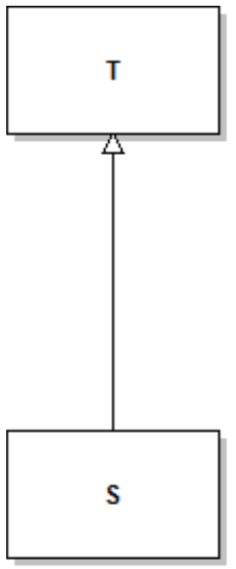
\includegraphics[width=0.55\linewidth]{figures/intro/Lis.png}
  \end{wrapfigure}
  \imp{In other words}:
  \begin{itemizenosep}
      \item Whenever you work with an instance of type T, you should not be
    surprised if you effectively work with an instance of type S
      \item An instance of type S can be used at all places where an instance of type T is expected
  \end{itemizenosep}
  \imp{Consequences}: Overriding methods need to satisfy (at least) the rules specified by the base class
\end{sectionbox}
\begin{defnbox}\nospacing
  \begin{defn}[Variance]\label{defn:Variance}
    Is a term applied to the expected behavior of subtypes in a class hierarchy containing complex types.
  \end{defn}
\end{defnbox}

%%% Local Variables:
%%% mode: latex
%%% TeX-master: "../formulary"
%%% End:

   \appendtographicspath{
          {java/figures/}
          {java/figures/basics/}
          {java/figures/oop/}
          {java/figures/stochastic/}
          }
\section{Basics}
\begin{defnbox}\nospacing
  \begin{defn}[Resolution]
    Is a rule of inference.
  \end{defn}
\end{defnbox}
\begin{defnbox}\nospacing
  \begin{defn}[Type]\label{defn:Type}
    defines a behavior but no implementation.\\
    (Java: Types are defined by classes)
  \end{defn}
\end{defnbox}
\begin{defnbox}\nospacing
  \begin{defn}[Subtyping]\label{defn:}
    Are specializations of Types and define a \rd{is-a} relationship.\\
    (Java: Subtyping is defined by subclassing, i.e. each subclass also defines a subtype)
  \end{defn}
\end{defnbox}
\begin{defnbox}\nospacing
  \begin{defn}[Java Method Signature]\label{defn:}
    Is the method name and the number, type and order of its parameters:
    \begin{mintlinebox}{java}
      methodName(Type1, Type2,...)
    \end{mintlinebox}
  \end{defn}
\end{defnbox}
\begin{notebox}[Note]\nospacing
  Return types, name of the arguments and thrown exceptions are not considered to be a part of the method signature. 
\end{notebox}
\begin{defnbox}\nospacing
  \begin{defn}[Method Declaration]\label{defn:methodDeclaration}
  Is a declaration of a function i.e.\ declares an identifier and its types,\ldots
    \begin{mintlinebox}{java}
      visibility |\optal|static|\optar| returnType methodName (args);
    \end{mintlinebox}
  \end{defn}
\end{defnbox}
\begin{defnbox}\nospacing
  \begin{defn}[Variable\blacksl Reference Declaration]\label{defn:referenceVariable}
    In java the only way to access an object is through a reference variable.
    \begin{mintlinebox}{java}
      StaticType reference;
    \end{mintlinebox}
    A reference is not an object, thus no memory is allocated for an object of
    the Type \javainline/StaticType/.
    of the reference.
    \begin{figure}[H]
      \vspace{-5pt}
      \centering
      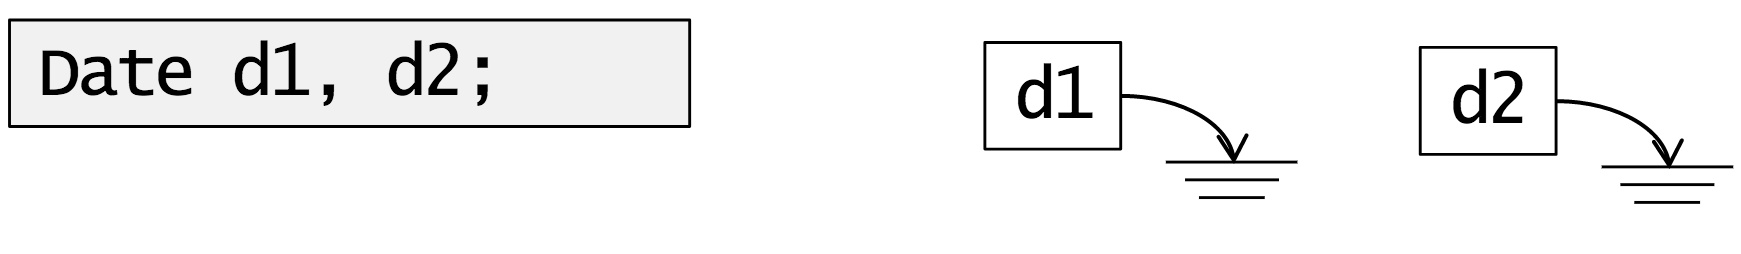
\includegraphics[width=.7\textwidth]{java/figures/basics/reference.png}
    \end{figure}
  \end{defn}
\end{defnbox}
\begin{notebox}[Note]\nospacing
  \begin{itemizenosep}
      \item Do not confuse C++ references with java references in Java variables are
  called (by convention) references.
      \item Reference variables are sort of C++ pointers but we can not do
    pointer arithmetic's on it e.g.\ \cppinline/ptr++/
      \item Reference Variables are of size:
    \begin{itemizenosep}
        \item 32-bit on a 32-bit JVM
        \item 32-bit of 64-bit on a 64-bit JVM, depending on the configuration
    \end{itemizenosep}
  \end{itemizenosep}
\end{notebox}
\begin{defnbox}\nospacing
  \begin{defn}[Static Type]\leavevmode
    A reference variable is declared to be of a specific type and that type,
    known as static type can never be changed.\leavevmode\\
    \ctr{Static type = type of reference variable}
  \end{defn}
\end{defnbox}
\begin{corbox}\nospacing
  \begin{cor}[Guarantees of Static Type]
    When a variable is declared as being of a particular type, then we have a
    language-enforced guarantee that any \textit{object} referenced by that
    reference variable will have (at least) all the features of that
    \textit{type}.\\
    $\Rightarrow$ \textit{dynamic type} needs to provide methods of \textit{static type}.
  \end{cor}  
\end{corbox}
\begin{defnbox}\nospacing
  \begin{defn}[Instanciation \javainline/new/]
    The new operator instantiates a class by dynamically allocating memory (=allocation at run time on the heap)
    for a new object and returns a reference to that memory.
    \begin{mintlinebox}{java}
      new MyClass();
    \end{mintlinebox}
    This reference can then be stored in/assigned to a (reference \cref{defn:referenceVariable}) variable.
    \begin{mintlinebox}{java}
      Type ref = new MyClass();
    \end{mintlinebox}
  \end{defn}
\end{defnbox}
\begin{notebox}[Note]\nospacing
  In Java, all class objects must be dynamically allocated.
\end{notebox}
%%% Local Variables:
%%% mode: latex
%%% TeX-master: "../../formulary"
%%% End:

\section*{Object Oriented Programming \rb{OOP}}
% ------------------------------------------------------------------------------ 
\subsection{Principles}
\begin{defnbox}\nospacing
  \begin{defn}[Encapsulation]\label{defn:encapsulation}\leavevmode
    \begin{itemizenosep}
      \item Methods and data are combined in classes
      \item Not unique to OOP
    \end{itemizenosep}
  \end{defn}
\end{defnbox}
\subsection{Class Basics}
\subsubsection{Static}
\label{subsubsec:Static}
\begin{defnbox}\nospacing
  \begin{defn}[Static Fields]\label{defn:staticFields}
    Per class fields, accessible via class (or instance)
    \begin{itemizenosep}
        \item Bound to class (available even if no instance has been created)
        \item Only one copy of the attribute (identical for all instances)
        \item Initialization per default with zero (0 / 0.0 / false / null) 
    \end{itemizenosep}
    \begin{mintlinebox}{java}
      static Type ref;
    \end{mintlinebox}
  \end{defn}
\end{defnbox}
\begin{stylebox}[Constants]\nospacing
  Declare constants as \javainline/static final/ fields.
\end{stylebox}
\begin{defnbox}\nospacing
  \begin{defn}[Static Methods]\label{defn:staticFields}
    Per Class methods, accessible via class (or instance):
    \begin{mintlinebox}{java}
      static ResultType Name(args){ Body }
    \end{mintlinebox}
    \begin{itemizenosep}
        \item No \javainline/this/
        \item No access to instance attributes \& methods
    \end{itemizenosep}
  \end{defn}
\end{defnbox}
\begin{stylebox}\nospacing
  Do not use instances to access static fields or methods.
\end{stylebox}
\subsubsection{Class Initialization}
\begin{sectionbox}[Upon loading o the class]\nospacing
  
\end{sectionbox}
\subsection{Inheritance}
\begin{defnbox}\nospacing
  \begin{defn}[\tc{black}{\normalfont{(Implementation Aspect)}}
    \\Code Inheritance\blacksl Extension\blacksl Subclassing]\leavevmode
    \begin{itemizenosep}
        \item Subclasses add new fields \& methods
        \item Subclasses have more (specialized) attributes \& operations
        \item Implementation aspect
    \end{itemizenosep}
    \imp{Class}: defines a type \imp{and} implementation
  \end{defn}
\end{defnbox}
\begin{defnbox}\nospacing
  \begin{defn}[\tc{black}{\normalfont{(Design Aspect)}}
    \\Interface Inheritance\blacksl Specialization\blacksl Subtyping]\leavevmode
    \begin{itemizenosep}
        \item Types define a set of objects
        \item Subtypes are specializations of this Type
        \item Inheritance of behavioral aspects
    \end{itemizenosep}
    \imp{Interface}: defines type
  \end{defn}
\end{defnbox}
\begin{defnbox}\nospacing
  \begin{defn}[\javainline/extends/]\label{defn:extends}\leavevmode\\
    Define new class by extending existing classes.\\
    In Java only one base class can be specified to inherit from.
    Extension inherits all fields and methods from the base class.
  \end{defn}
\end{defnbox}
\subsubsection{Polymorphism}
\begin{defnbox}\nospacing
  \begin{defn}[Type Checking]
    The process of verifying and enforcing the constraints of types
  \end{defn}
\end{defnbox}
\begin{defnbox}\nospacing
  \begin{defn}[Statically Typed Languages]
    Is a language where the type of a variable is known at compile time.\\
    For some languages this means that we as programmer must specify of what type each variable is.\\
    \Advantage\ can do type-checking during compile time by the compiler, and therefore a lot of trivial bugs are caught at a very early stage.\\
    \imp{Examples}: C, C++, Java
  \end{defn}
\end{defnbox}
\begin{defnbox}\nospacing
  \begin{defn}[Dynamically Typed Languages]
     If the type is associated with/depends on run-time \imp{values}, and not named variables/fields/etc\\
     \Advantage\ we do not have to specify types every time.\\
     \Drawback\ do type checking at run-time
  \end{defn}
\end{defnbox}
\label{subsubsec:Polymorphism}
\begin{defnbox}\nospacing
  \begin{defn}[Polymorphism]\label{defn:polymorphism}
    Polymorphism allows operations to be performed on objects without needing to know which class the object belongs to,
    provided that we can guarantee that the class implements the specified type.
  \end{defn}
\end{defnbox}
\begin{defnbox}\nospacing
  \begin{defn}[Polymorphic Assignment]
    Instances of an extended class can be assigned to references of type base
    class:
    \begin{mintlinebox}{java}
      BaseClass ref = new extendedClass();
    \end{mintlinebox}
  \end{defn}
\end{defnbox}
\begin{defnbox}\nospacing
  \begin{defn}[Dynamic Type]\label{defn:dynamicType}
    Is the type of the object assigned to a reference variable.\\
    Dynamic types of reference variables may change with every assignment.\\
    $\text{Dynamic Type}\subseteq\text{Static Type}$ as the dynamic type most
    full fill at least the guarantees of the static type.
  \end{defn}
\end{defnbox}
\begin{defnbox}\nospacing
  \begin{defn}[Static Binding]
    Is type resolution based on the static type of a variable reference.
  \end{defn}
\end{defnbox}
\begin{defnbox}\nospacing
  \begin{defn}[Static Binding and Overloading]
    If we overload a method in Java, the compiler will produce a version for
    each overloaded function \rd{signature}.\\
    The resolution of the method signature (not to the actual implementation) of the
    method is done during compile time and does hence depend on the \rd{static type}
    passed to the method $\Rightarrow$ static binding
    \begin{mintlinebox}{java}
      StaticTypeOfa a = new DynamicTypeOfa();
      a.methodToResolveTo(StaticTypeOfb b);
    \end{mintlinebox}
    \javainline/staticTypeOfb/ decides which overloaded method to call.
  \end{defn}
\end{defnbox}
\begin{defnbox}\nospacing
  \begin{defn}[\\Dynamic Type Binding and Overloading]
    The runtime chooses a function implementation
    \begin{numberlistnosep}
        \item Based on the function \rd{signature} chosen at compile time
      (dynamic binding)
        \item Depending on the dynamic type of the object referenced by
      \javainline/a/ in order to chose an actual implementation of
      \begin{mintlinebox}{java}
          DynamicTypeOfa.methodToResolveTo(StaticTypeOfb b)
      \end{mintlinebox}
    \end{numberlistnosep}
  \end{defn}
\end{defnbox}
\begin{notebox}[Note]\nospacing
  For non-overloaded methods only the dynamic type of the reference variable
  decides which method to call.
\end{notebox}
\begin{codeboxNl}[Dynamic Type Inference]{java}
  if( ref instanceof Type)
\end{codeboxNl}
\begin{codeboxcomment}[Type Casts]{0.3}{java}{
    A runtime error is thrown if the dynamic type of \javainline/ref/ is not a
    Type or extension thereof.
  }
  (Type) ref;
\end{codeboxcomment}
\subsection{Abstract Classes}
\begin{defnbox}\nospacing
  \begin{defn}[Abstract Methods]
    Are methods that only define a signature/are only a declaration:
    \begin{mintlinebox}{java}
      visibility abstract retrunType methodName();
    \end{mintlinebox}
    \begin{itemizenosep}
        \item Define methods to be implemented in subclasses
        \item Can only be declared in \javainline/abstract/ classes
        \item Cannot be \javainline/private/ as private methods cannot be overridden
        \item Cannot be \javainline/static/ as static methods cannot be overridden
    \end{itemizenosep}
  \end{defn}
\end{defnbox}
\begin{defnbox}\nospacing
  \begin{defn}[Abstract Classes]
    Are classes that how stand in an ``\rd{is-a}'' relationship with their subclasses:
    \begin{itemizenosep}
      \item Cannot be instantiated
      \item Usually have one or more abstract methods
      \item May have attributes, constructors, non-abstract methods 
    \end{itemizenosep}
    \begin{mintlinebox}{java}
      visibility abstract class Name{ Body }
    \end{mintlinebox}
  \end{defn}
\end{defnbox}
\begin{notebox}[Note]\nospacing
  An abstract class must not necessarily have an abstract method.\\
  Useful to declare classes abstract that cannot/may not be initiated but (but extended)
\end{notebox}
\begin{notebox}[Note: \normalfont{Derived Classes}]\nospacing
  \begin{itemizenosep}
      \item Have to override (implement) all \javainline/abstract/ methods
      \item Or have to be declared abstract as well, if not all abstract methods
    are overridden.
  \end{itemizenosep}
\end{notebox}
\begin{notebox}[Note]\nospacing
  Arrays of an abstract base type may be instantiated sine No instances are
  created (only reference variables)
  \begin{mintlinebox}{java}
    ContainerType[] name = new ContainerType[Number]
  \end{mintlinebox}
\end{notebox}
\begin{stylebox}[Usage]\nospacing
  \begin{itemizenosep}
      \item Want to share code among several closely related classes.
      \item You expect that classes that extend your abstract class have many
    common methods or fields or require access modifiers other than public (such
    as protected and private).
      \item You want to declare non-static or non-final fields. This enables you to define methods that can access and modify the state of the object to which they belong.
  \end{itemizenosep}
\end{stylebox}
\subsection{Interfaces}
\begin{defnbox}\nospacing
  \begin{defn}[Interfaces=pure abstract class]\label{defn:interfaces}
    Have to be implemented by the class that uses the interface and represent a
    ``\rd{can-do}'' relationship:
    \begin{itemizenosep}
      \item Have only \javainline/public/ and \javainline/abstract/ methods
      \item Attributes are by default \javainline/public,static/ and
    \javainline/final/
      \item No constructors $\Rightarrow$ instantiated ($\neq$ declared)
    \end{itemizenosep}
    \imp{Definition}:
    \begin{mintlinebox}{java}
      public intreface ClassName{ Body; }
    \end{mintlinebox}
    \imp{Implementation}:
    \begin{mintlinebox}{java}
      class ClassName implements IntefaceName{ Body; }
    \end{mintlinebox}
    \begin{itemizenosep}
        \item All methods defined in the declared interface have to be
      implemented unless its another interface adding more functionality
        \item A class may implement multiple interfaces
    \end{itemizenosep}
  \end{defn}
\end{defnbox}
\begin{notebox}[Note: Java 8 default methods]\nospacing
  Can be implemented inside interfaces and are able access other methods.
  Allows to extend interfaces without breaking existing classes that implement
  the interface.
\end{notebox}
\begin{stylebox}\nospacing
  Use \javainline/@override/ to implement the methods.
\end{stylebox}
\begin{stylebox}[Usage]\nospacing
  \begin{itemizenosep}
    \item You expect that unrelated classes would implement a piece of
  functionality. 
    \item Want to specify the behavior of a particular data type, but not concerned about who implements its behavior.
  \end{itemizenosep}
\end{stylebox}
\begin{notebox}[Interfaces as function arguments]\nospacing
  Methods with Interfaces as type can be called with any class implementation
  that interface.
\end{notebox}
\begin{notebox}[Interface Reference]\nospacing
  Interfaces can be used as reference variable for all subclasses \imp{but} be
  care-full if the reference object implements another interface we will not be
  able to call its functions unless we use an implicit cast.\\
  Check if referenced object implements an interface: \javainline/ref instanceof aInterface/
\end{notebox}
\begin{codeboxNl}[Interaface Variable]{java}
  TypeImplementingAandB ref = new TypeImplementingAandB()
  InterfaceTypeA refA = ref;
  InterfaceTypeB refB = ref;
  refA instanceof InterfaceTypeB // True as ref implements B
  refA.methodOfTypeImplementingAandB() // works
  refA.methodOfB() // does not work
  ((InterfaceTypeB)refA).methodOfB() // works
\end{codeboxNl}
\begin{sectionbox}[Intrefaces and Abstract Classes]\nospacing
  \begin{itemize}
      \item \javainline/Interface/: provides a type
      \item \javainline/abstract Class/ semi finished component that contains
    default implementations
    \begin{itemizenosep}
        \item which can be used in subclasses
        \item which can be overriden in subclasses
    \end{itemizenosep}
  \end{itemize}
  \begin{figure}[H]
    \centering
    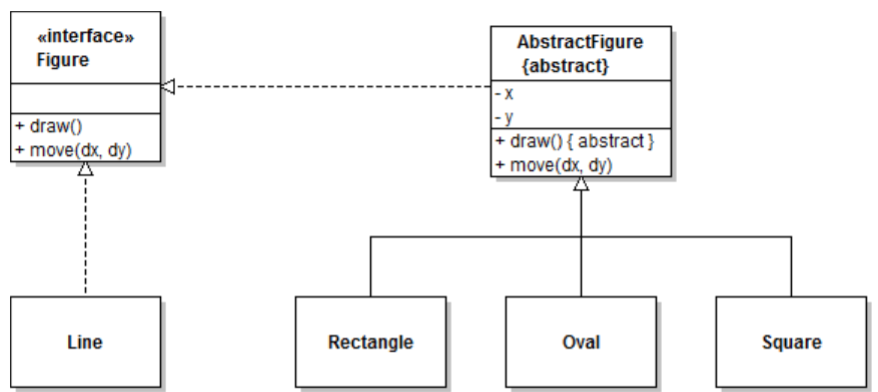
\includegraphics[width=1.0\textwidth]{java/figures/oop/abstractInterface.png}
  \end{figure}
\end{sectionbox}
\begin{notebox}[Abstract Classes vs. Interfaces]\nospacing
  \begin{itemizenosep}
      \item Abstract Classes
    \begin{itemizenosep}
        \item A class may extend only one abstract class
        \item Abstract classes may contain attributes \& concrete implementations
    \end{itemizenosep}
      \item Interfaces
    \begin{itemizenosep}
        \item A class may implement sever interfaces
        \item Abstract classes may contain no implementations 
    \end{itemizenosep}
  \end{itemizenosep}
\end{notebox}
\begin{defnbox}\nospacing
  \begin{defn}[Marker Interface]\label{defn:markerInerface}
    Is an empty interface, that can be used to add a certain
    attribute/characteristic to a class that can be checked with
    \javainline/instanceof/ e.g.\ RandomAcess 
  \end{defn}
\end{defnbox}
\begin{defnbox}\nospacing
  \begin{defn}[Functional Interface \javainline/@FunctionalInterface/]\label{defn:functionalInterface}
    Is an interface with a single abstract method:
    \begin{mintlinebox}{java}
      @FunctionalInterface
      public interface InterfaceName{
        visibility returnType methodName(args);
      }
    \end{mintlinebox}
  \end{defn}
\end{defnbox}
\begin{notebox}[Notes]\nospacing
  \begin{itemizenosep}
      \item The annotation \javainline/@FunctionalInterface/ allows compilers to generate an
  error if the interface does not satisfy the conditions of a functional
  interface.
    \item Default methods are not abstract and do not count.
  \end{itemizenosep}
\end{notebox}
\begin{sectionbox}[Lambda Expressions and Functional Interfaces]\nospacing
  
\end{sectionbox}
%%% Local Variables:
%%% mode: latex
%%% TeX-master: "../../formulary"
%%% End:

% ------------------------------------------------------------------------------ 
%%% Local Variables:
%%% mode: latex
%%% TeX-master: "../formulary"
%%% End:

\newpage
% ==============================================================================
% Design Patterns
% ==============================================================================
\section{Behavioral Patters}
\label{subsubsec:Behavirol}
\begin{defnbox}\nospacing
  \begin{defn}[Behavioral Patterns]
    These design patterns are specifically concerned with communication between objects.
  \end{defn}
\end{defnbox}
%%% Local Variables:
%%% mode: latex
%%% TeX-master: "../formulary"
%%% End:

\subsection{Observer\slash Listener\slash Publish-Subscriber}
\label{subsubsec:Observer}
% java -jar /opt/plantuml/plantuml.jar -verbose -tlatex observer.txt; mv observer.latex observer.tex
\begin{figure}[H]	
  \centering
    \resizebox{\linewidth}{!}{\tikzset{font=\Huge}\documentclass{standalone}
\usepackage{tikz}
\usepackage{aeguill}
\begin{document}
% generated by Plantuml 1.2018.12      
\definecolor{plantucolor0000}{RGB}{254,254,206}
\definecolor{plantucolor0001}{RGB}{168,0,54}
\definecolor{plantucolor0002}{RGB}{169,220,223}
\definecolor{plantucolor0003}{RGB}{0,0,0}
\definecolor{plantucolor0004}{RGB}{180,167,229}
\definecolor{plantucolor0005}{RGB}{173,209,178}
\definecolor{plantucolor0006}{RGB}{251,251,119}
\begin{tikzpicture}[yscale=-1
,pstyle0/.style={color=plantucolor0001,fill=plantucolor0000,line width=1.5pt}
,pstyle2/.style={color=plantucolor0001,line width=1.5pt}
,pstyle4/.style={color=plantucolor0001,fill=plantucolor0005,line width=1.0pt}
,pstyle5/.style={color=plantucolor0001,fill=plantucolor0006,line width=1.0pt}
,pstyle6/.style={color=plantucolor0001,line width=1.0pt}
,pstyle7/.style={color=plantucolor0001,fill=plantucolor0001,line width=1.0pt}
]
\draw[pstyle0] (62pt,109pt) rectangle (190.3385pt,221.0234pt);
\draw[color=plantucolor0001,fill=plantucolor0002,line width=1.0pt] (96.3127pt,125pt) ellipse (11pt and 11pt);
\node at (96.3127pt,125pt)[]{\textbf{\Large A}};
\node at (114.6045pt,118.0156pt)[below right,color=black]{\textit{Subject}};
\draw[pstyle2] (63pt,141pt) -- (189.3385pt,141pt);
\node at (68pt,145pt)[below right,color=black]{+observers};
\draw[pstyle2] (63pt,161.8047pt) -- (189.3385pt,161.8047pt);
\node at (68pt,165.8047pt)[below right,color=black]{+attach(o : Obs)};
\node at (68pt,178.6094pt)[below right,color=black]{+detach(o : Obs)};
\node at (68pt,191.4141pt)[below right,color=black]{+notifyObs()};
\node at (68pt,204.2188pt)[below right,color=black]{\textit{getSubjectStatus()}};
\draw[pstyle0] (298.5pt,134.5pt) rectangle (395.7421pt,195.3047pt);
\draw[color=plantucolor0001,fill=plantucolor0004,line width=1.0pt] (313.5pt,150.5pt) ellipse (11pt and 11pt);
\node at (313.5pt,150.5pt)[]{\textbf{\Large I}};
\node at (327.5pt,143.5156pt)[below right,color=black]{\textit{Observer}};
\draw[pstyle2] (299.5pt,166.5pt) -- (394.7421pt,166.5pt);
\draw[pstyle2] (299.5pt,174.5pt) -- (394.7421pt,174.5pt);
\node at (304.5pt,178.5pt)[below right,color=black]{\textit{update()}};
\draw[pstyle0] (73pt,282pt) rectangle (222.8118pt,342.8047pt);
\draw[pstyle4] (88pt,298pt) ellipse (11pt and 11pt);
\node at (88pt,298pt)[]{\textbf{\Large C}};
\node at (102pt,291.0156pt)[below right,color=black]{ConcreteSubject};
\draw[pstyle2] (74pt,314pt) -- (221.8118pt,314pt);
\draw[pstyle2] (74pt,322pt) -- (221.8118pt,322pt);
\node at (79pt,326pt)[below right,color=black]{getSubjecdtStatus()};
\draw[pstyle0] (262.5pt,282pt) rectangle (423.9pt,342.8047pt);
\draw[pstyle4] (277.5pt,298pt) ellipse (11pt and 11pt);
\node at (277.5pt,298pt)[]{\textbf{\Large C}};
\node at (291.5pt,291.0156pt)[below right,color=black]{ConcreteObserver};
\draw[pstyle2] (263.5pt,314pt) -- (422.9pt,314pt);
\draw[pstyle2] (263.5pt,322pt) -- (422.9pt,322pt);
\node at (268.5pt,326pt)[below right,color=black]{update()};
\draw[pstyle5] (284.5pt,8pt) -- (284.5pt,48.2656pt) -- (343pt,48.2656pt) -- (347pt,134.2998pt) -- (351pt,48.2656pt) -- (409.4636pt,48.2656pt) -- (409.4636pt,18pt) -- (399.4636pt,8pt) -- (284.5pt,8pt);
\draw[pstyle5] (399.4636pt,8pt) -- (399.4636pt,18pt) -- (409.4636pt,18pt) -- (399.4636pt,8pt);
\node at (290.5pt,13pt)[below right,color=black]{may be an};
\node at (290.5pt,28.1328pt)[below right,color=black]{abstract class};
\draw[pstyle5] (6pt,15.5pt) -- (6pt,40.6328pt) -- (122pt,40.6328pt) -- (126pt,108.8568pt) -- (130pt,40.6328pt) -- (245.8pt,40.6328pt) -- (245.8pt,25.5pt) -- (235.8pt,15.5pt) -- (6pt,15.5pt);
\draw[pstyle5] (235.8pt,15.5pt) -- (235.8pt,25.5pt) -- (245.8pt,25.5pt) -- (235.8pt,15.5pt);
\node at (12pt,20.5pt)[below right,color=black]{may be interface or concrete};
\draw[pstyle6] (203.2192pt,165pt) ..controls (203.2192pt,165pt) and (285.4477pt,165pt) .. (285.4477pt,165pt);
\draw[pstyle7] (298.4477pt,165pt) -- (289.4477pt,161pt) -- (293.4477pt,165pt) -- (289.4477pt,169pt) -- (298.4477pt,165pt) -- cycle;
\draw[pstyle6] (293.4477pt,165pt) -- (285.4478pt,165pt);
\draw[pstyle7] (190.2192pt,165pt) -- (196.2192pt,169pt) -- (202.2192pt,165pt) -- (196.2192pt,161pt) -- (190.2192pt,165pt) -- cycle;
\draw[pstyle6] (131.5pt,241.1842pt) ..controls (131.5pt,241.1842pt) and (131.5pt,281.6437pt) .. (131.5pt,281.6437pt);
\draw[pstyle6] (124.5001pt,241.1842pt) -- (131.5pt,221.1842pt) -- (138.5001pt,241.1842pt) -- (124.5001pt,241.1842pt) -- cycle;
\draw[color=plantucolor0001,line width=1.0pt,dash pattern=on 7.0pt off 7.0pt] (347pt,215.5621pt) ..controls (347pt,215.5621pt) and (347pt,281.9771pt) .. (347pt,281.9771pt);
\draw[pstyle6] (340.0001pt,215.5621pt) -- (347pt,195.5621pt) -- (354.0001pt,215.5621pt) -- (340.0001pt,215.5621pt) -- cycle;
\draw[pstyle6] (223.1132pt,313pt) ..controls (223.1132pt,313pt) and (257.4237pt,313pt) .. (257.4237pt,313pt);
\draw[pstyle7] (262.4237pt,313pt) -- (253.4237pt,309pt) -- (257.4237pt,313pt) -- (253.4237pt,317pt) -- (262.4237pt,313pt) -- cycle;
\end{tikzpicture}
\end{document}
}
\end{figure}
\begin{intentbox}[Intent]\nospacing
  \begin{itemize}
      \item Consistency assurance between cooperating objects without connecting them too much.
      \item  One-to-many relation between objects which allows to inform the
        dependent objects about state changes
  \end{itemize}
\end{intentbox}
\begin{codeboxNl}[Observer]{java}
  interface Observer{
    void update ();
  }
\end{codeboxNl}
\begin{codeboxNl}[Subject]{java}
class Subject {
  private List <Observer > observers = new ArrayList <Observer >();

  public void addObserver(Observer o) {
    // method of List
    observers.add(o);
  }

  public void removeObserver(Observer o) {
    // method of List
    observers.remove(o);
  }

  protected void notifyObservers () {
    // inform all Observers that we have changed
    for(Observer obs : observers) {
      // Let (concrete) observers handle it
      obs.|\ul{update}| ();
    }
  }
}
\end{codeboxNl}
\begin{codeboxNl}[Concrete Subject]{java}
class ConcSubject extends Subject {
  private int state;
  public int getState (){
    return state;
  }

  public void setState(int val){
    state = val;
    notifyObservers();
  }
}
\end{codeboxNl}
\begin{codeboxNl}[Concrete Observer]{java}
class ConcObserver implements Observer {
  private |\ul[ulc4]{ConcSubject s}|;
  ConcObserver (ConcSubject s){
    this.s = s;
    s.addObserver(this);
  }

  public void |\ul{update}| (){
    // take appropriate steps
  }
}
\end{codeboxNl}
\begin{partbox}[Participants]\nospacing
  \begin{itemizenosep}
      \item \imp{Observer}: typically an interface that declares methods to
      handle notifications.
      \item \imp{Subject}: maybe concrete or interface knows its observers over
      the observer interface (guarantee that the method \ul{\javainline{update}}
      exists).
        \item \imp{Concrete Observer}:
      \begin{itemize}
          \item Handles state changes of its observable
          \item Implements the observer interface to keep its state consistent with
                the subject
          \item May maintain a \ul[ulc4]{reference} to a concrete subject (pull-model)
        \todo[inline]{Check if ref is really because of pull model}
      \end{itemize}
      \item \imp{Concrete Subject}: Implements/extends Subject and hence can:
      \begin{itemize}
          \item attach observers
          \item detach observers
          \item call the method notify if its state changes\\
          (e.g.\ in a set method)
      \end{itemize}
  \end{itemizenosep}
\end{partbox}
\begin{consequencebox}[Consequence]
  \begin{itemizenosep}
    \item Subject does not care about the number of observers $\Rightarrow$
    notifications are broadcast.
    \item A simple state change/operation may lead to a (unwanted) cascade of
  updates.\\
  $\rightarrow$ beware of cyclic dependencies see
  \todo[inline]{add cref}
  \end{itemizenosep}
\end{consequencebox}
\begin{notebox}[Note]\nospacing
  \begin{itemizenosep}
      \item Thus it is up to the observer to handle or \imp{ignore}
    notifications.
      \item When should \javainline{notifyObservers} be called?
    \begin{itemizenosep}
        \item \imp{Automatically}: at every state change\\
      $\Rightarrow$ many updates
        \item \imp{Explicitly}: after a set of changes\\
      $\Rightarrow$ responsibility e.g.\
      \begin{itemize}
          \item Asynchronous at idle times 
          \item Use a boolean flag \javainline{changed}, that can be set in
          order to test if object has changed see \cref{subsubsec:Java.util.Observable}
        \todo[inline]{clarify why or what for?}
      \end{itemize}
    \end{itemizenosep}
  \end{itemizenosep}
\end{notebox}
\subsubsection{One or Many Observables}
\begin{figure}[H]	
  \centering
  \resizebox{\linewidth}{!}{\tikzset{font=\Huge}\documentclass{standalone}
\usepackage{tikz}
\usepackage{aeguill}
\begin{document}
% generated by Plantuml 1.2018.12      
\definecolor{plantucolor0000}{RGB}{254,254,206}
\definecolor{plantucolor0001}{RGB}{168,0,54}
\definecolor{plantucolor0002}{RGB}{169,220,223}
\definecolor{plantucolor0003}{RGB}{0,0,0}
\definecolor{plantucolor0004}{RGB}{3,128,72}
\definecolor{plantucolor0005}{RGB}{132,190,132}
\definecolor{plantucolor0006}{RGB}{180,167,229}
\definecolor{plantucolor0007}{RGB}{255,0,0}
\begin{tikzpicture}[yscale=-1
,pstyle0/.style={color=plantucolor0001,fill=plantucolor0000,line width=1.5pt}
,pstyle2/.style={color=plantucolor0001,line width=1.5pt}
,pstyle4/.style={color=plantucolor0004,fill=plantucolor0005,line width=1.0pt}
]
\draw[pstyle0] (6pt,8pt) rectangle (148.3385pt,120.0234pt);
\draw[color=plantucolor0001,fill=plantucolor0002,line width=1.0pt] (34.138pt,24pt) ellipse (11pt and 11pt);
\node at (34.138pt,24pt)[]{\textbf{\Large A}};
\node at (51.0576pt,17.0156pt)[below right,color=black]{\textit{Observable}};
\draw[pstyle2] (7pt,40pt) -- (147.3385pt,40pt);
\draw[color=plantucolor0004,line width=1.0pt] (17pt,51.9023pt) ellipse (3pt and 3pt);
\node at (26pt,44pt)[below right,color=black]{observers};
\draw[pstyle2] (7pt,60.8047pt) -- (147.3385pt,60.8047pt);
\draw[pstyle4] (17pt,72.707pt) ellipse (3pt and 3pt);
\node at (26pt,64.8047pt)[below right,color=black]{attach(o : Obs)};
\draw[pstyle4] (17pt,85.5117pt) ellipse (3pt and 3pt);
\node at (26pt,77.6094pt)[below right,color=black]{detach(o : Obs)};
\draw[pstyle4] (17pt,98.3164pt) ellipse (3pt and 3pt);
\node at (26pt,90.4141pt)[below right,color=black]{notifyObs()};
\node at (26pt,103.2188pt)[below right,color=black]{\textit{getSubjectStatus()}};
\draw[pstyle0] (268.5pt,33.5pt) rectangle (365.7421pt,94.3047pt);
\draw[color=plantucolor0001,fill=plantucolor0006,line width=1.0pt] (283.5pt,49.5pt) ellipse (11pt and 11pt);
\node at (283.5pt,49.5pt)[]{\textbf{\Large I}};
\node at (297.5pt,42.5156pt)[below right,color=black]{\textit{Observer}};
\draw[pstyle2] (269.5pt,65.5pt) -- (364.7421pt,65.5pt);
\draw[pstyle2] (269.5pt,73.5pt) -- (364.7421pt,73.5pt);
\node at (274.5pt,77.5pt)[below right,color=black]{\textit{update()}};
\draw[color=plantucolor0001,line width=1.0pt] (148.0338pt,64pt) ..controls (148.0338pt,64pt) and (263.2019pt,64pt) .. (263.2019pt,64pt);
\draw[color=plantucolor0001,fill=plantucolor0001,line width=1.0pt] (268.2019pt,64pt) -- (259.2019pt,60pt) -- (263.2019pt,64pt) -- (259.2019pt,68pt) -- (268.2019pt,64pt) -- cycle;
\node at (163.6179pt,65pt)[below right,color=black]{observers};
\draw[color=black,fill=black,line width=1.0pt] (238.5064pt,71.0664pt) -- (244.5064pt,74.0664pt) -- (238.5064pt,77.0664pt) -- (238.5064pt,71.0664pt) -- cycle;
\node at (156.2823pt,48.1933pt)[below right,color=plantucolor0007]{\textbf{?}};
\node at (252.5886pt,47.785pt)[below right,color=black]{*};
\end{tikzpicture}
\end{document}
}
\end{figure}
\begin{sectionbox}[0\ldots 1 : *]\nospacing
  \begin{itemizenosep}
      \item Subject/Observable is usually passed to constructor of the Concrete
    Observer ($\Rightarrow$ \ul[ulc4]{reference}).
      \item 
  \end{itemizenosep}
\end{sectionbox}
\begin{sectionbox}[* : *]\nospacing
  \begin{itemizenosep}
      \item If we want that observers can observe multiple subjects and if these
    observers may be able to ignore certain events from those subjects,
    then the observer need to know the source of an update event.\\
    Moreover if arguments are passed to the Observables, then the observer needs
    to know:
    \begin{itemize}
        \item The arguments
        \item The source of the event
    \end{itemize}
  \end{itemizenosep}
\end{sectionbox}
\begin{figure}[H]	
  \centering
  \resizebox{\linewidth}{!}{\tikzset{font=\Huge}\documentclass{standalone}
\usepackage{tikz}
\usepackage{aeguill}
\begin{document}
% generated by Plantuml 1.2018.12      
\definecolor{plantucolor0000}{RGB}{254,254,206}
\definecolor{plantucolor0001}{RGB}{168,0,54}
\definecolor{plantucolor0002}{RGB}{169,220,223}
\definecolor{plantucolor0003}{RGB}{0,0,0}
\definecolor{plantucolor0004}{RGB}{3,128,72}
\definecolor{plantucolor0005}{RGB}{132,190,132}
\definecolor{plantucolor0006}{RGB}{255,0,0}
\definecolor{plantucolor0007}{RGB}{180,167,229}
\begin{tikzpicture}[yscale=-1
,pstyle0/.style={color=plantucolor0001,fill=plantucolor0000,line width=1.5pt}
,pstyle2/.style={color=plantucolor0001,line width=1.5pt}
,pstyle4/.style={color=plantucolor0004,fill=plantucolor0005,line width=1.0pt}
]
\draw[pstyle0] (6pt,8pt) rectangle (170.5237pt,120.0234pt);
\draw[color=plantucolor0001,fill=plantucolor0002,line width=1.0pt] (44.1214pt,24pt) ellipse (11pt and 11pt);
\node at (44.1214pt,24pt)[]{\textbf{\Large A}};
\node at (63.2595pt,17.0156pt)[below right,color=black]{\textit{Observable}};
\draw[pstyle2] (7pt,40pt) -- (169.5237pt,40pt);
\draw[color=plantucolor0004,line width=1.0pt] (17pt,51.9023pt) ellipse (3pt and 3pt);
\node at (26pt,44pt)[below right,color=black]{observers};
\draw[pstyle2] (7pt,60.8047pt) -- (169.5237pt,60.8047pt);
\draw[pstyle4] (17pt,72.707pt) ellipse (3pt and 3pt);
\node at (26pt,64.8047pt)[below right,color=black]{attach(o : Obs)};
\draw[pstyle4] (17pt,85.5117pt) ellipse (3pt and 3pt);
\node at (26pt,77.6094pt)[below right,color=black]{detach(o : Obs)};
\draw[pstyle4] (17pt,98.3164pt) ellipse (3pt and 3pt);
\node at (26pt,90.4141pt)[below right,color=black]{notifyObs(};
\node at (90.2207pt,90.4141pt)[below right,color=plantucolor0006]{Object args};
\node at (159.7237pt,90.4141pt)[below right,color=black]{)};
\node at (26pt,103.2188pt)[below right,color=black]{\textit{getSubjectStatus()}};
\draw[pstyle0] (206.5pt,27pt) rectangle (398.3264pt,100.6094pt);
\draw[color=plantucolor0001,fill=plantucolor0007,line width=1.0pt] (265.5422pt,43pt) ellipse (11pt and 11pt);
\node at (265.5422pt,43pt)[]{\textbf{\Large I}};
\node at (286.0422pt,36.0156pt)[below right,color=black]{\textit{Observer}};
\draw[pstyle2] (207.5pt,59pt) -- (397.3264pt,59pt);
\draw[pstyle2] (207.5pt,67pt) -- (397.3264pt,67pt);
\node at (212.5pt,71pt)[below right,color=black]{\textit{update(}};
\node at (212.5pt,83.8047pt)[below right,color=plantucolor0006]{\textit{Observable src, Object args}};
\node at (387.5264pt,83.8047pt)[below right,color=black]{\textit{)}};
\draw[color=plantucolor0001,line width=1.0pt] (171.238pt,65pt) ..controls (171.238pt,65pt) and (201.4327pt,65pt) .. (201.4327pt,65pt);
\draw[color=plantucolor0001,fill=plantucolor0001,line width=1.0pt] (206.4327pt,65pt) -- (197.4327pt,61pt) -- (201.4327pt,65pt) -- (197.4327pt,69pt) -- (206.4327pt,65pt) -- cycle;
\node at (178.4336pt,49.4662pt)[below right,color=black]{*};
\node at (190.6096pt,49.4444pt)[below right,color=black]{*};
\end{tikzpicture}
\end{document}
}
\end{figure}
\begin{codeboxNl}[Many vs Many]{java}
protected void notifyObservers(Object args){
    for(Observer obs : observers){
        obs.update(this, args);
    }
}
\end{codeboxNl}
\subsubsection{Push vs Pull Model}
\begin{sectionbox}[\tc{section}{Push-Model}]\nospacing
  \begin{itemizenosep}
      \item The subject (i.e.\ the Observable) sends the observer on notification all the data it will need.
      The observer doesn't need to query the subject for information.
      \item Observable must know which information is needed by the observers
      in order for them to act appropriately (or Observable sends all data)
  \end{itemizenosep}
\end{sectionbox}
\begin{sectionbox}[\tc{section}{Pull-Model}]\nospacing
  \begin{itemizenosep}
      \item 
      In the pull model, the subject merely notifies the observer that something
      happened, and the observer queries the subject based on that, to get the information it needs.
      \item Observable send only information about what has changed
      \item Observer has to access the Observable state (via \ul[ulc4]{reference})
  \end{itemizenosep}
\end{sectionbox}
\todo[inline]{maybe add pros and cons}
\subsection*{Pitfalls}
\label{subsubsec:Pitfalls}
\subsubsection{Java.util.Observable}
\label{subsubsec:Java.util.Observable}
\begin{sectionbox}\nospacing
  Provides an implementation of an Observable that can be used.\\
  \imp{But} it is never used!\\
  \imp{Problem}: multiple inheritance is in java not possible, thus
  \javainline{Java.util.Observable} can only be implemented if extension is not
  defined in its own inheritance hierarchy.\\
  \imp{Solution}: \tc{section}{composite} twin class (\cref{subsection:Composite}).\\
    $\Rightarrow$ code duplication $\Rightarrow$ \javainline{Java.util.Observable}
  is not used.
\end{sectionbox}
\begin{codeboxNl}[\texttt{Java.util.Observable}]{java}
public interface Observer {
  void update(Observable o, Object arg);
}

public class Observable {
  private boolean changed = false;

  // Marks this Observable as having been changed
  protected void setChanged() { changed = true; }

  // Indicates that this object has no longer changed,
  // or that it has already notified all of its observers
  // of its most recent change.
  protected void clearChanged() { changed = false; }

  // Tests if this object has changed.
  public boolean hasChanged() { return changed; }

  // If this object has changed, as indicated by the
  // hasChanged method, then notify all of its observers
  // and then call the clearChanged method to indicate
  // that this object has no longer changed.
  public void notifyObservers(Object arg) {
    if (!changed) return;
    // See section on ConcurrentModificationException
    Object[] copy = obs.toArray();
    clearChanged(); // before notification!
    for (int i = copy.length-1; i>=0; i--)
      ((Observer)copy[i]).update(this, arg);
  }
}
\end{codeboxNl}
\todo[inline]{Add observable twin class solution after we studied again composite}
\subsubsection{ConcurrentModificationException}
\label{subsubsec:ConcurrentModificationException}
\begin{defnbox}\nospacing
  \begin{defn}[\javainline{ConcurrentModificationException}]
    We cannot change a list e.g.\ add/remove while iterating over it.\\
    \imp{Example}: Once Observer and notify.
  \end{defn}
\end{defnbox}
\begin{defnbox}\nospacing
  \begin{defn}[OnceObserver]\label{defn:OnceObserver}
    Is an observer that only observers for a single notification.\\
    $\Rightarrow$ removes itself afterwards.
  \end{defn}
\end{defnbox}
\begin{codeboxNl}[OnceObserver]{java}
public class OnceObserver implements Observer {
  public void update(Observable |$\overbrace{\text{source}}^{\mathclap{\text{Conc. Observerable}}}$|, Object arg) {
        // take appropriate steps once
        source.|\ul[ulc5]{removeObserver}|(this);
  }
}
\end{codeboxNl}
\begin{codeboxcomment}[Problem]{0.74}{java}{\imp{Problem}: we cannot remove an
    observer from \javainline{obs} while iterating over it}
protected void notifyObservers(Object arg){
  for(Observer obs : observers){
    obs.update(this, arg);
  }
}
\end{codeboxcomment}
\begin{sectionbox}[Solutions]\nospacing
  \begin{circlelistnosep}
      \item Perform the notifications on a copy of the observer list.
      \item Delay add/remove Observer calls.
      \item Copy the observer list upon modification.
  \end{circlelistnosep}
\end{sectionbox}
\begin{defnbox}\nospacing
  \begin{defn}[Java list to array]
    Returns an array containing all of the elements in this list in proper sequence (from first to last element).
    \begin{mintlinebox}{java}
      java.util.ArrayList.toArray(a T[])
    \end{mintlinebox}
    \javainline{a}: is the array into which the elements of the list are to be
    stored, if it is big enough; otherwise, a new array of the same runtime type is allocated for this purpose.
  \end{defn}
\end{defnbox}
\todo[inline]{understand better how this works}
\begin{codeboxNl}[Copy Solution]{java}
protected void notifyObservers(){
  Observer[] copy;
  copy = observers.toArray(new Observer[observers.size()]);
  for (Observer obs : copy){
    obs.update(this);
  }
}
\end{codeboxNl}
\begin{codeboxNl}[Alternative]{java}
protected void notifyObservers(){
  for(Observer o : new ArrayList<>(observables)){
    o.update(this);
  }
}
\end{codeboxNl}
\todo[inline]{maybe add Mutation or gamble, must likly not important}
\begin{defnbox}\nospacing
  \begin{defn}[Copy on write list]
    Thread-safe variant of ArrayList in which
    all mutative operations are implemented by making a fresh copy of the
    underlying array.
  \end{defn}
\end{defnbox}
\begin{codeboxNl}[Best Solution]{java}
  private List<Observer> observers = new CopyOnWriteArrayList<>();
  public void addObserver(Observer o) { observers.add(o); }
  public void removeObserver(Observer o) { observers.remove(o); }

  protected void notifyObservers(Object arg) {
    for(Observer obs : observers) {
      obs.update(this, arg);
    }
  }
\end{codeboxNl}
\subsubsection{Cyclic dependencies}
\label{subsubsec:CyclicDependencies}
\begin{sectionbox}[Problem]\nospacing
  If we have a cyclic dependency we will end up in an endless loop of notifying
  and updating, unless we take appropriate measures.
\begin{figure}[H]
  \centering
  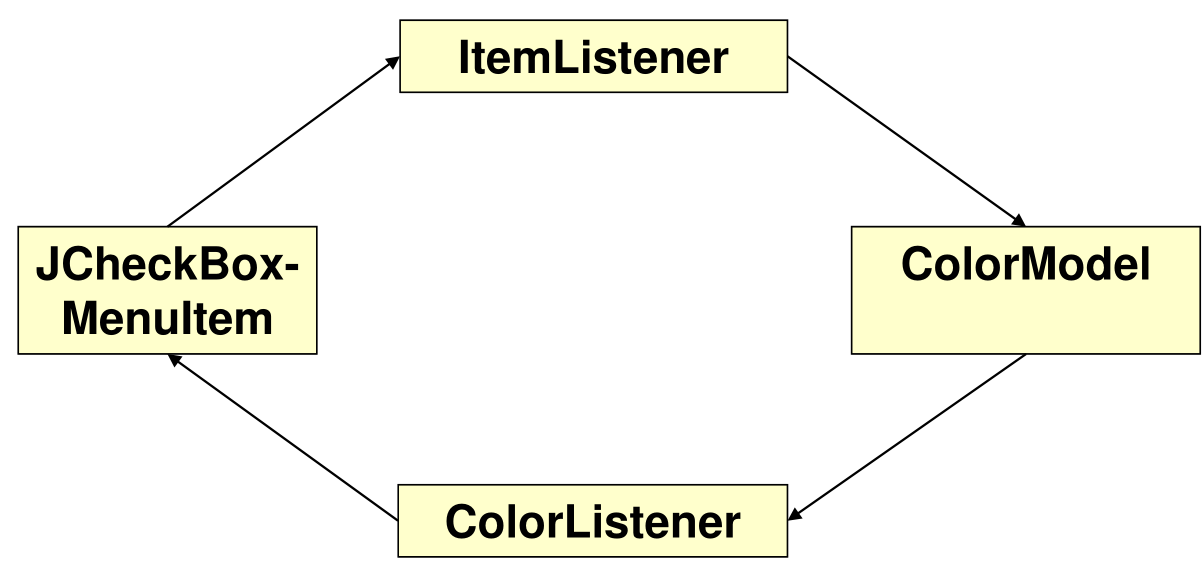
\includegraphics[width=0.7\columnwidth]{figures/cyclic_dependency.png}
  \label{fig:cyclic_dependency}
\end{figure}
\imp{General Rule}: Propagate changes only if the model really changed!
\end{sectionbox}
\begin{sectionbox}[Solution 1: Color Listener]\nospacing
    Break recursion inside the listener: e.g.\ we
    check inside the color listener if the color really changed, or is still the
    same $\Rightarrow$ recursion or nothing happens anyway.
      \begin{mintlinebox}{java}
        // update method of listener
       public void colorValueChanged(Color c){
          if (isSelected() OR_OPRATOR !c.equals(this.color))
          // If the color really changed and isSelected is true
          // select the checkbox menu item
            setSelected(c.equals(this.color));
        }
      \end{mintlinebox}
      \imp{Note}: not recommended to check inside the listener, as we may have
      many different kinds of listener.
\end{sectionbox}
\begin{sectionbox}[Solution 2: ItemListener flag]\nospacing
  Same as Solution 1 (but now for the ItemListener) but we use a flag instead of checking the actual value and:
      \begin{mintlinebox}{java}
       private boolean updating = false;
       public void itemstateChanged(ItemEvent e){
         if (!updating){
            updating = true;
            if(e.getStateChanged() == ItemEvent.SELECTED)
                 |\ul{model}|.setColor(color);
          }
          updating = false;
        }
      \end{mintlinebox}
      \imp{Note}: not recommended to check inside the listener, as we may have
      many different kinds of listener.
\end{sectionbox}
\begin{sectionbox}[Solution 3: Concrete Model]\nospacing
    Break recursion inside the Model: e.g.\ we check inside a subclass of JCheckBoxMenueItem
    if the performed action has already been performed and if not we can call
    the super method:
      \begin{mintlinebox}{java}
       public void setSelected(boolean b){
          if (b != isSelected())
            super.setSelected(b);
        }
      \end{mintlinebox}
      \imp{Note}: recommended as we usually have one model and lots of different listeners.
\end{sectionbox}
\begin{sectionbox}[Solution 4: Color Model]\nospacing
      \begin{mintlinebox}{java}
       public class |\ul{ColorModel}|{
         private Color color;
         public void setColor(Color color){
            if (c.equals(this.color)){
              this.color = color;
              notify(color);
            }
         }
      }
      \end{mintlinebox}
      \imp{Note}: recommended as we usually have one model and lots of different listeners.
\end{sectionbox}
\begin{notebox}[Note]\nospacing
  \javainline{isSelected() OR_OPRATOR !c.equals(this.color)} can be written as
  \javainline{isSelected() != c.equals(this.color)}
\end{notebox}
\begin{notebox}[Note: Solution 5]\nospacing
  Use ActionListener instead of an ItemListener: Actions are only triggered
  by keyboard or mouse events.
\end{notebox}
\subsubsection{Causality of Changes}
\label{subsubsec:CausalityofChanges}
\begin{sectionbox}[Problem]\nospacing
  How can we make sure that notifications of the model will be handled by the
  observers in the same order as they were applied to the models.
\end{sectionbox}
\begin{sectionbox}[Solution]\nospacing
  \begin{itemizenosep}
      \item Queuing of state changes: model becomes asynchronous\ldots difficult
      to program 
      \item Queuing of notifications 
      \item Prohibit state changes during notification
  \end{itemizenosep}
\end{sectionbox}
\subsubsection{Memory Management}
\label{subsubsec:MemoryManagement}
\begin{sectionbox}\nospacing
  Is automatic in java if no more reference to an object exists.\\
  $\Rightarrow$ need to detach all observers/listeners for clean up.
\end{sectionbox}
\todo[inline]{add twin classes}
\subsection{Actions}
\begin{defnbox}\nospacing
  \begin{defn}[Action]\label{defn:Action}
    Is the measure to take onto and actionEvent.
  \end{defn}
\end{defnbox}
\subsubsection{ActionListener and performed actions}
\begin{defnbox}\nospacing
  \begin{defn}[Adapter Class]\label{defn:AdapterClass}\leavevmode\\
    Java adapter classes provide the default implementation of ActionListener
    interfaces and implement the \javainline{public abstract void actionPerformed(ActionEvent e)} method.
  \end{defn}
\end{defnbox}
\begin{sectionbox}\nospacing
 There exist multiple ways to specify how an action Listener should react to an
 an (action) event.\\
 \imp{E.g.} \javainline{java.awt.event.ActionListener} is a
 functional interface \cref{defn:functionalInterface} with a single abstract method\\
 \javainline{public abstract void actionPerformed(ActionEvent e)}; \\
 which defines what action to take onto an event.\\
 In order to write an Action Listener, we can:
 \begin{circlelistnosep}
     \item \textbf{\tc{section}{Use the subject directly}}: the subject must implement the ActionListener
      and hence implement the method \javainline{actionPerdormed} or
     \item \textbf{\tc{section}{We use an Adapter Class}} (\cref{defn:AdapterClass}): that implements the action Listerner
   Interface and register it inside the subject or
     \item We use anonymous classes of the ActionListener and register it inside
   the subject.
     \item \textbf{\tc{section}{We use lambda expressions}} (\cref{defn:FunctionalInterfacesAndLambda}): of the ActionListener and register it
   inside the subject.
 \end{circlelistnosep}
\end{sectionbox}
\begin{codebox}[Direct Implementation]{java}
  public class Subject implements ActionListener {
    |\optldots|
    public void actionPerformed(ActionEvent e) {
      if(e.getSource() == push) handlePush();
      else if(e.getSource() == pop) handlePop();
    }
\end{codebox}
\begin{codebox}[Adapter Implementation]{java}
class PushListener implements ActionListener {
  public void actionPerformed(ActionEvent e) { |\optldots| }
}
subj_obj.addActionListener(instanceOfMyClass);
\end{codebox}
\begin{codebox}[Anonymous Implementation]{java}
subj_obj.addActionListener(new ActionListener() {
  public void actionPerformed(ActionEvent ae) {|\optldots|}
  });
\end{codebox}
\begin{codebox}[Lambda Implementation]{java}
subj_obj.addActionListener((ActionEvent e) -> {
  |\optldots|
  });
  // or even just
subj_obj.addActionListener(e -> {
  |\optldots|
  });
\end{codebox}
\begin{notebox}[Note: multi-method listeners]\nospacing
  Anonymous interfaces still need to be used for implementing multi-method interfaces.
\end{notebox}
%%% Local Variables:
%%% mode: latex
%%% TeX-command-extra-options: "-shell-escape"
%%% TeX-master: "../formulary"
%%% End:

\subsection{State Patterns}
\label{subsubsec:StatePatterns}
\begin{figure}[H]	
  \centering
    \resizebox{\linewidth}{!}{\tikzset{font=\Huge}\documentclass{standalone}
\usepackage{tikz}
\usepackage{aeguill}
\begin{document}
% generated by Plantuml 1.2018.12      
\definecolor{plantucolor0000}{RGB}{254,254,206}
\definecolor{plantucolor0001}{RGB}{168,0,54}
\definecolor{plantucolor0002}{RGB}{173,209,178}
\definecolor{plantucolor0003}{RGB}{0,0,0}
\definecolor{plantucolor0004}{RGB}{169,220,223}
\begin{tikzpicture}[yscale=-1
,pstyle0/.style={color=plantucolor0001,fill=plantucolor0000,line width=1.5pt}
,pstyle1/.style={color=plantucolor0001,fill=plantucolor0002,line width=1.0pt}
,pstyle2/.style={color=plantucolor0001,line width=1.5pt}
,pstyle4/.style={color=plantucolor0001,line width=1.0pt}
,pstyle5/.style={color=plantucolor0001,fill=plantucolor0001,line width=1.0pt}
]
\draw[pstyle0] (6pt,8pt) rectangle (129.6941pt,120.0234pt);
\draw[pstyle1] (37.2424pt,24pt) ellipse (11pt and 11pt);
\node at (37.2424pt,24pt)[]{\textbf{\Large C}};
\node at (54.8518pt,17.0156pt)[below right,color=black]{Context};
\draw[pstyle2] (7pt,40pt) -- (128.6941pt,40pt);
\node at (12pt,44pt)[below right,color=black]{state};
\draw[pstyle2] (7pt,60.8047pt) -- (128.6941pt,60.8047pt);
\node at (12pt,64.8047pt)[below right,color=black]{+methodA()};
\node at (12pt,77.6094pt)[below right,color=black]{+allMethods()};
\node at (12pt,90.4141pt)[below right,color=black]{+setState(State s)};
\node at (12pt,103.2188pt)[below right,color=black]{+getstate()};
\draw[pstyle0] (165pt,27pt) rectangle (243.1419pt,100.6094pt);
\draw[color=plantucolor0001,fill=plantucolor0004,line width=1.0pt] (184.0464pt,43pt) ellipse (11pt and 11pt);
\node at (184.0464pt,43pt)[]{\textbf{\Large A}};
\node at (198.9456pt,36.0156pt)[below right,color=black]{\textit{State}};
\draw[pstyle2] (166pt,59pt) -- (242.1419pt,59pt);
\draw[pstyle2] (166pt,67pt) -- (242.1419pt,67pt);
\node at (171pt,71pt)[below right,color=black]{-methodA()};
\node at (171pt,83.8047pt)[below right,color=black]{-methodB()};
\draw[pstyle0] (44pt,180pt) rectangle (186.4632pt,228pt);
\draw[pstyle1] (59pt,196pt) ellipse (11pt and 11pt);
\node at (59pt,196pt)[]{\textbf{\Large C}};
\node at (73pt,189.0156pt)[below right,color=black]{ConcreteState1};
\draw[pstyle2] (45pt,212pt) -- (185.4632pt,212pt);
\draw[pstyle2] (45pt,220pt) -- (185.4632pt,220pt);
\draw[pstyle0] (221pt,180pt) rectangle (363.4632pt,228pt);
\draw[pstyle1] (236pt,196pt) ellipse (11pt and 11pt);
\node at (236pt,196pt)[]{\textbf{\Large C}};
\node at (250pt,189.0156pt)[below right,color=black]{ConcreteState2};
\draw[pstyle2] (222pt,212pt) -- (362.4632pt,212pt);
\draw[pstyle2] (222pt,220pt) -- (362.4632pt,220pt);
\draw[pstyle4] (143.407pt,64pt) ..controls (146.1887pt,64pt) and (148.9704pt,64pt) .. (151.7521pt,64pt);
\draw[pstyle5] (164.7705pt,64pt) -- (155.7705pt,60pt) -- (159.7705pt,64pt) -- (155.7705pt,68pt) -- (164.7705pt,64pt) -- cycle;
\draw[pstyle4] (159.7705pt,64pt) -- (151.7705pt,63.9999pt);
\draw[pstyle5] (130.1562pt,64pt) -- (136.1562pt,68pt) -- (142.1562pt,64pt) -- (136.1562pt,60pt) -- (130.1562pt,64pt) -- cycle;
\draw[pstyle4] (169.6379pt,118.0528pt) ..controls (156.0476pt,139.4308pt) and (141.1249pt,162.9046pt) .. (130.3139pt,179.9107pt);
\draw[pstyle4] (163.7462pt,114.2727pt) -- (180.3833pt,101.1499pt) -- (175.5609pt,121.7835pt) -- (163.7462pt,114.2727pt) -- cycle;
\draw[pstyle4] (238.1767pt,118.372pt) ..controls (251.5603pt,139.6642pt) and (266.2218pt,162.9892pt) .. (276.8582pt,179.9107pt);
\draw[pstyle4] (232.0684pt,121.8078pt) -- (227.3513pt,101.1499pt) -- (243.9213pt,114.3574pt) -- (232.0684pt,121.8078pt) -- cycle;
\end{tikzpicture}
\end{document}
}
\end{figure}
\begin{intentbox}[Intent]\nospacing
    Context related behavior depending on the current state
\end{intentbox}
\begin{partbox}[Participants]\nospacing
  \begin{itemizenosep}
      \item \imp{Context}: is the concrete thing (e.g.\ Vending Machine, Ventilator) that has a reference/stores the concrete state
      and acts depending on it by calling the \javainline{request} or \javainline{doAction} method of its current state reference.
      \item \imp{Abstract/Interface State}: is
    \begin{itemizenosep}
        \item Is an interface that will be implemented by the \textit{concrete states} and defines all the possible actions
        that each \textit{concrete state} may be able to perform or
          \item An abstract base class if
        \begin{itemize}
            \item we want to define default behaviors of the shared methods:
             \begin{mintlinebox}{java}
               privat void doAction1(|\optc{args}|){
                 throw new IllegalStateException();
               }
             \end{mintlinebox}
            \item the concrete states store shared similar attributes/methods that we do not want to define inside the context.
        \end{itemize}
    \end{itemizenosep}
    \item \imp{Concrete State}: Implements the methods of the \textit{state interface}
  \end{itemizenosep}
\end{partbox}
\begin{notebox}[Note]\nospacing
  \begin{itemizenosep}
      \item Contexts may hold multiple different states e.g.\ light state as well as temperature state.
      \item The possible actions declared inside the state interface/abstract class \ul{may take a context object} as argument
      in order to change the current state, if they are not defined inside the context (see \tc{section}{State changes} section).
      \item Interfaces allow only public methods before Java9, may be another reason for using abstract classes.
  \end{itemizenosep}
\end{notebox}
\begin{codeboxNl}[Context]{java}
  class Context{
    State state;
    
    public void setState(State s){
      this.state = s;
    }

    public State getState(){
      return state;
    }

    public doAction1(){
      state.doAction1(|\ul{\opta{this}}|);
    }

  }
\end{codeboxNl}
\begin{codeboxNl}[State]{java}
  abstract class State {
    privat void doAction1(|\ul{\opta{Context cur}}|,|\optc{args}|){
      throw new IllegalStateException();
    }
  }
}
\end{codeboxNl}
\subsection*{State Changes}
\subsubsection{Decentralized}
\begin{sectionbox}\nospacing
  May be initiated by the \rd{concrete state} method $\Rightarrow$
  \begin{itemizenosep}
    \item Concrete state object needs a reference to the \textit{context} in order to set its state:
  \end{itemizenosep}
\end{sectionbox}
  \begin{codeboxNl}[Context]{java}
    class Context{
      State state;
      |\optldots|
      public doActions(){
        state.doAction1(this);
        state.doAction2(this);
      }

    }
  \end{codeboxNl}
  \begin{codeboxNl}[State]{java}
    interface State {
      public |\optc{retType}| doAction1(Context cur,|\optc{args}|);
      public |\optc{retType}| doAction2(Context cur,|\optc{args}|);
    }
  }
  \end{codeboxNl}
  \begin{codeboxNl}[\rd{Concrete State}]{java}
    concStateA implementes State {
      public state doAction1(Context cur, |\optc{args}|);
          // do somthing
          cur.setState(new StateB());
    }
  }
  \end{codeboxNl}
\begin{sectionbox}\nospacing
 \begin{itemizenosep}
    \item \imp{Or} the state returns the new state when running an action which gets then set by the context
 \end{itemizenosep} 
\end{sectionbox}
\begin{codeboxNl}[Context]{java}
  class Context{
    State s;
    |\optldots|
    public doActions(){
      s = state.doAction1();
      s = state.doAction2();
    }
  }
\end{codeboxNl}
\begin{sectionbox}\nospacing
 \begin{itemizenosep}
     \item \imp{Or} the state and Concrete States are defined inside context class, thus concrete
      states can directly set state of the context:
 \end{itemizenosep} 
\end{sectionbox}
\begin{codeboxNl}[\rd{Concrete State}]{java}
class Context{
  State s;
  |\optldots|
  concStateA implementes State {
    public state doAction1(|\optc{args}|);
        // do somthing
        s = setState(new StateB());
  }
  |\optldots|
}
\end{codeboxNl}
\subsubsection{Centralized}
\begin{sectionbox}\nospacing
  Transitions are initiated by the context, state should be informed that it gets activated or deactivated. 
    \begin{codeboxNl}[DrawTool (State)]{java}
      public interface DrawTool{
        void activate();
        void deactivate();
      }
    \end{codeboxNl}
    \begin{codeboxNl}[DrawView (Context)]{java}
      DrawTool tool; // current state
      
      public void setTool(DrawTool tool){ // set conc state;
        if(tool == null) throw new IllegalArgumentException();
        if(this.tool != null) this.tool.deactivate();
        this.tool = tool;
        this.tool.activate();
      }
    \end{codeboxNl}
\end{sectionbox}
\begin{notebox}[Note]\nospacing
  If the initial state is set in the constructor of the context we can omit:
  \javainline{if(this.tool != null) this.tool.deactivate();}
\end{notebox}
\subsection*{Creation of State Objects}
\subsubsection{States are created on demand}
\begin{sectionbox}\nospacing
 \begin{codebox}{java}
   public void stateMethod1(Context cur){
     cur.setState(new StateB());
   }
 \end{codebox} 
\end{sectionbox}
\subsubsection{States are stored}
\begin{sectionbox}\nospacing
  States are stored in variable or list that is accessible by all concrete states
  $\Rightarrow$ thus states are for example stored inside context.
\end{sectionbox}
 \begin{codebox}[Context]{java}
   class Context{
     State s;
     |\optldots|
     private final State CONC_STATE_A = new CStateA();
     private final State CONC_STATE_B = new CStateB();
     private final State INIT = new InitState();
 }
 \end{codebox} 
 \begin{codebox}[Abstract State Class]{java}
   public void stateMethod1(Context cur){
     cur.setState(c.INIT);
   }
 \end{codebox} 
 \begin{codebox}[Abstract State Class]{java}
   public void stateMethod2(Context cur){
     throw new IllegalStateException();
   }
 \end{codebox} 
\begin{notebox}[Examples]\nospacing
  \begin{itemizenosep}
      \item DrawTool (drawing state)
      \item DrawGrid (constrain the mouse coordinates)
      \item Handles (CTRL/SHIFT pressed)
  \end{itemizenosep}
\end{notebox}
%%% Local Variables:
%%% mode: latex
%%% TeX-master: "../formulary"
%%% End:

\subsection{Strategy Patterns}
\label{subsubsec:StrategyPatterns}
\begin{figure}[H]	
  \centering
    \resizebox{\linewidth}{!}{\tikzset{font=\Huge}\documentclass{standalone}
\usepackage{tikz}
\usepackage{aeguill}
\begin{document}
% generated by Plantuml 1.2018.12      
\definecolor{plantucolor0000}{RGB}{254,254,206}
\definecolor{plantucolor0001}{RGB}{168,0,54}
\definecolor{plantucolor0002}{RGB}{173,209,178}
\definecolor{plantucolor0003}{RGB}{0,0,0}
\definecolor{plantucolor0004}{RGB}{180,167,229}
\begin{tikzpicture}[yscale=-1
,pstyle0/.style={color=plantucolor0001,fill=plantucolor0000,line width=1.5pt}
,pstyle1/.style={color=plantucolor0001,fill=plantucolor0002,line width=1.0pt}
,pstyle2/.style={color=plantucolor0001,line width=1.5pt}
,pstyle4/.style={color=plantucolor0001,line width=1.0pt}
,pstyle5/.style={color=plantucolor0001,fill=plantucolor0001,line width=1.0pt}
]
\draw[pstyle0] (6pt,8pt) rectangle (130.9098pt,81.6094pt);
\draw[pstyle1] (37.7894pt,24pt) ellipse (11pt and 11pt);
\node at (37.7894pt,24pt)[]{\textbf{\Large C}};
\node at (55.5204pt,17.0156pt)[below right,color=black]{Context};
\draw[pstyle2] (7pt,40pt) -- (129.9098pt,40pt);
\node at (12pt,44pt)[below right,color=black]{strategy};
\draw[pstyle2] (7pt,60.8047pt) -- (129.9098pt,60.8047pt);
\node at (12pt,64.8047pt)[below right,color=black]{+contextMethod()};
\draw[pstyle0] (166pt,14.5pt) rectangle (286.9773pt,75.3047pt);
\draw[color=plantucolor0001,fill=plantucolor0004,line width=1.0pt] (193.7783pt,30.5pt) ellipse (11pt and 11pt);
\node at (193.7783pt,30.5pt)[]{\textbf{\Large I}};
\node at (210.6179pt,23.5156pt)[below right,color=black]{\textit{Strategy}};
\draw[pstyle2] (167pt,46.5pt) -- (285.9773pt,46.5pt);
\draw[pstyle2] (167pt,54.5pt) -- (285.9773pt,54.5pt);
\node at (172pt,58.5pt)[below right,color=black]{\textit{strategyMethod()}};
\draw[pstyle0] (42pt,142pt) rectangle (208.8552pt,202.8047pt);
\draw[pstyle1] (57pt,158pt) ellipse (11pt and 11pt);
\node at (57pt,158pt)[]{\textbf{\Large C}};
\node at (71pt,151.0156pt)[below right,color=black]{ConcreteStrategy1};
\draw[pstyle2] (43pt,174pt) -- (207.8552pt,174pt);
\draw[pstyle2] (43pt,182pt) -- (207.8552pt,182pt);
\node at (48pt,186pt)[below right,color=black]{-strategyMethod()};
\draw[pstyle0] (244pt,142pt) rectangle (410.8552pt,202.8047pt);
\draw[pstyle1] (259pt,158pt) ellipse (11pt and 11pt);
\node at (259pt,158pt)[]{\textbf{\Large C}};
\node at (273pt,151.0156pt)[below right,color=black]{ConcreteStrategy2};
\draw[pstyle2] (245pt,174pt) -- (409.8552pt,174pt);
\draw[pstyle2] (245pt,182pt) -- (409.8552pt,182pt);
\node at (250pt,186pt)[below right,color=black]{-strategyMethod()};
\draw[pstyle4] (144.4055pt,45pt) ..controls (147.1893pt,45pt) and (149.9732pt,45pt) .. (152.757pt,45pt);
\draw[pstyle5] (165.7854pt,45pt) -- (156.7854pt,41pt) -- (160.7854pt,45pt) -- (156.7854pt,49pt) -- (165.7854pt,45pt) -- cycle;
\draw[pstyle4] (160.7854pt,45pt) -- (152.7854pt,44.9999pt);
\draw[pstyle5] (131.1445pt,45pt) -- (137.1445pt,49pt) -- (143.1445pt,45pt) -- (137.1445pt,41pt) -- (131.1445pt,45pt) -- cycle;
\draw[pstyle4] (189.8575pt,91.2566pt) ..controls (176.5428pt,108.0648pt) and (161.8351pt,126.6314pt) .. (149.8447pt,141.7679pt);
\draw[pstyle4] (184.4021pt,86.87pt) -- (202.308pt,75.5394pt) -- (195.3762pt,95.5632pt) -- (184.4021pt,86.87pt) -- cycle;
\draw[pstyle4] (263.1425pt,91.2566pt) ..controls (276.4572pt,108.0648pt) and (291.1649pt,126.6314pt) .. (303.1553pt,141.7679pt);
\draw[pstyle4] (257.6238pt,95.5632pt) -- (250.692pt,75.5394pt) -- (268.5979pt,86.87pt) -- (257.6238pt,95.5632pt) -- cycle;
\end{tikzpicture}
\end{document}
}
\end{figure}
\begin{intentbox}[Intent]\nospacing
  \begin{itemizenosep}
      \item Allow to change algorithms independently of the clients
      \item Support extensibility with new algorithms
      \item Make algorithms interchangeable
  \end{itemizenosep}
\end{intentbox}
\begin{sectionbox}[Which problem does it solve]\nospacing
  \begin{minipage}[t]{0.45\textwidth}
  Strategy pattern is an alternative to specialization of context
  class which:
  \begin{itemizenosep}
      \item violates the \rd{Single Responsibility Principle}
      \item prevents interchanging the strategy of a context dynamically, as
    subclassing statically defines the binding between context and strategy
  \end{itemizenosep}
  \end{minipage}
  \begin{minipage}[t]{0.5\textwidth}
  \begin{figure}[H]
    \centering
    \vspace{-1em}
      \resizebox{\linewidth}{!}{\documentclass{standalone}
\usepackage{tikz}
\usepackage{aeguill}
\begin{document}
% generated by Plantuml 1.2018.12      
\definecolor{plantucolor0000}{RGB}{254,254,206}
\definecolor{plantucolor0001}{RGB}{168,0,54}
\definecolor{plantucolor0002}{RGB}{173,209,178}
\definecolor{plantucolor0003}{RGB}{0,0,0}
\begin{tikzpicture}[yscale=-1
,pstyle0/.style={color=plantucolor0001,fill=plantucolor0000,line width=1.5pt}
,pstyle1/.style={color=plantucolor0001,fill=plantucolor0002,line width=1.0pt}
,pstyle2/.style={color=plantucolor0001,line width=1.5pt}
,pstyle3/.style={color=plantucolor0001,line width=1.0pt}
]
\draw[pstyle0] (77pt,8pt) rectangle (164.6pt,68.8047pt);
\draw[pstyle1] (92pt,24pt) ellipse (11pt and 11pt);
\node at (92pt,24pt)[]{\textbf{\Large C}};
\node at (106pt,17.0156pt)[below right,color=black]{Context};
\draw[pstyle2] (78pt,40pt) -- (163.6pt,40pt);
\node at (83pt,44pt)[below right,color=black]{\textit{strategy}};
\draw[pstyle2] (78pt,60.8047pt) -- (163.6pt,60.8047pt);
\draw[pstyle0] (6pt,129pt) rectangle (103.9439pt,189.8047pt);
\draw[pstyle1] (21pt,145pt) ellipse (11pt and 11pt);
\node at (21pt,145pt)[]{\textbf{\Large C}};
\node at (35pt,138.0156pt)[below right,color=black]{ContextA};
\draw[pstyle2] (7pt,161pt) -- (102.9439pt,161pt);
\node at (12pt,165pt)[below right,color=black]{strategy};
\draw[pstyle2] (7pt,181.8047pt) -- (102.9439pt,181.8047pt);
\draw[pstyle0] (139pt,129pt) rectangle (236.593pt,189.8047pt);
\draw[pstyle1] (154pt,145pt) ellipse (11pt and 11pt);
\node at (154pt,145pt)[]{\textbf{\Large C}};
\node at (168pt,138.0156pt)[below right,color=black]{ContextB};
\draw[pstyle2] (140pt,161pt) -- (235.593pt,161pt);
\node at (145pt,165pt)[below right,color=black]{strategy};
\draw[pstyle2] (140pt,181.8047pt) -- (235.593pt,181.8047pt);
\draw[pstyle3] (94.605pt,86.8909pt) ..controls (86.8583pt,101.0932pt) and (78.6053pt,116.2237pt) .. (71.6493pt,128.9764pt);
\draw[pstyle3] (88.623pt,83.2393pt) -- (104.3454pt,69.0334pt) -- (100.9136pt,89.9433pt) -- (88.623pt,83.2393pt) -- cycle;
\draw[pstyle3] (147.795pt,86.8909pt) ..controls (155.659pt,101.0932pt) and (164.0371pt,116.2237pt) .. (171.0985pt,128.9764pt);
\draw[pstyle3] (141.4714pt,89.9211pt) -- (137.9069pt,69.0334pt) -- (153.7191pt,83.1393pt) -- (141.4714pt,89.9211pt) -- cycle;
\end{tikzpicture}
\end{document}
}
  \end{figure}
  \end{minipage}
\end{sectionbox}
\begin{partbox}[Participants]\nospacing
  \begin{itemizenosep}
      \item \imp{Context}: 
      is the real thing e.g.\
      \begin{itemize}
          \item A secure channel
          \item Container
          \item TransportationToAirport
      \end{itemize}
      that uses a concrete strategy.\\
      Thus it must have a reference/stores an instance of the concrete strategy.\\
      The name of the context method(s) depends on the context e.g.\
      \begin{itemize}
          \item encrypt, decrypt
          \item addLayoutComponent, minimumLayoutSize
          \item transport
      \end{itemize}
      and acts depending on it by calling the \javainline{request} or \javainline{doAction} method of its current state reference.
      \item \imp{Strategy/Algorithm Interface}: is
        usually an interface as we implement some functionality and do not have an
        ``is-a'' relationship.\\
        The strategy interface specifies which methods the algorithms may be
        able to perform.
    \item \imp{Concrete Algorithm}: Implements the methods of the \textit{Strategy interface}
  \end{itemizenosep}
\end{partbox}
\begin{notebox}[Note]\nospacing
  \begin{itemizenosep}
    \item Strategy methods may contain a \ul{reference} to the context as a parameter,
  in order to use a state full algorithm see
  \cref{subsubsec:statefullVsStateless}.
    \item Strategy Interface may be defined inside the context class.
  \end{itemizenosep}
\end{notebox}
\begin{codeboxNl}[Context]{java}
  class Context{
    private Strategy algorithm;
    
    public void setAlgorithm(Strategy a){
      if(a == 0){ // See also Null Object Pattern |\cref{subsubsec:NullObjectPattern}|
        throw new IllegalArgumentException();
      } 
      this.algorithm = a;
    }

    public State contextMethod1(){
      algorithm.doAction1()
    }

    public State contextMethod1(){
      algorithm.doAction1()
      algorithm.doAction2(|\ul{\opta{this}}|,|\optc{args}|)
      algorithm.doAction1()
    }

  }
\end{codeboxNl}
\begin{codeboxNl}[Strategy Interface]{java}
  interface class Strategy {
    privat void doAction1();
    privat void doAction2(|\ul{\opta{Context cur}}|,|\optc{args}|);
}
\end{codeboxNl}
\begin{codeboxNl}[Concrete Strategy]{java}
  class Algorithm1 implements Strategy {
    privat void doAction1(){|\ldots|};
    privat void doAction2(|\ul{\opta{Context cur}}|,|\optc{args}|){|\ldots|};
}
\end{codeboxNl}
\subsubsection{Statefull vs Stateless Strategys}
\label{subsubsec:statefullVsStateless}
\begin{sectionbox}\nospacing
\begin{figure}[H]
  \centering
  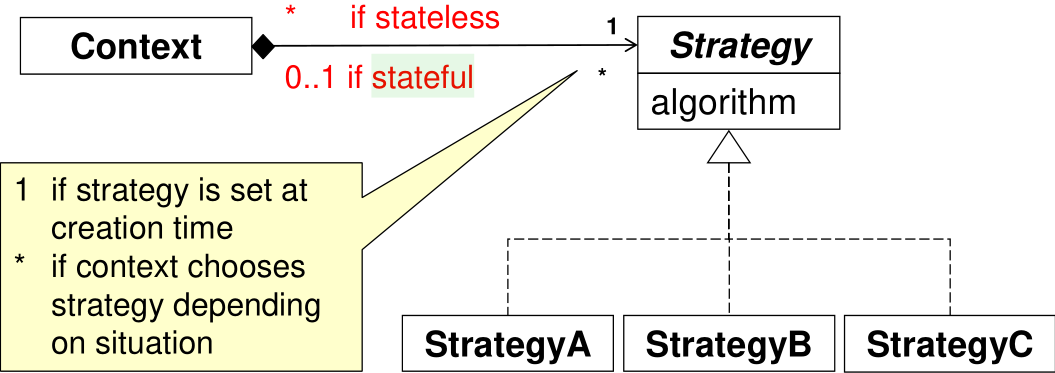
\includegraphics[width=1.0\columnwidth]{figures/strategyStatefulVsStateless.png}
  \label{fig:StatefullVsStateless}
\end{figure}
 \begin{itemizenosep}
     \item \rdb{Stateless} Strategy: does not store/have any state/context
   specific parameters $\Rightarrow$ strategy can be used from different
   contexts.\\
   \imp{Note}: in order to use parameters, strategy may \ul{access} state
   specific parameters of \textit{context} (but not itself!).
     \item \rdb{Statefull} Strategy: may store/have any state/context specific
   parameters $\Rightarrow$ cannot be exchanged between different contexts.
 \end{itemizenosep} 
\end{sectionbox}
\begin{sectionbox}[Strategy vs. State]\nospacing
\begin{minipage}[t]{0.45\textwidth}
  \imp{\tc{section}{Strategy}}
  \begin{itemize}
    \item Strategy is typically not aware of other concrete strategies
    \item Typically set only once
    \item Usually only one \textit{public} method
    \item Strategy may contain algorithm specific state
  \end{itemize}
\end{minipage}
\begin{minipage}[t]{0.45\textwidth}
  \imp{\tc{section}{State}}
  \begin{itemize}
      \item A concrete state may be aware of others $\Rightarrow$ transitions.
      \item Defines state-specific behavior
      \item Typically state changes at runtime
      \item State usually contains no state but accesses state in context
  \end{itemize}
\end{minipage}
\end{sectionbox}
%%% Local Variables:
%%% mode: latex
%%% TeX-master: "../formulary"
%%% End:

\subsection{Null Object Pattern}
\label{subsubsec:NullObjectPattern}
\begin{intentbox}[Intent]
  \imp{Motivation}: We do not want to litter the whole code with statements of
  the form \javainline{if(strategy!=null)} in order to check if a strategy is set.
  \begin{itemizenosep}
  \item
  Encapsulate the absence of an object/a strategy by providing a substitutable
  alternative that offers suitable default ``\textit{do noting}'' behavior
  \begin{itemizenosep}
      \item empty methods \javainline{{}}
      \item no strategy set error
  \end{itemizenosep}
  \end{itemizenosep}
\end{intentbox}
\begin{codeboxNl}{java}
public class NullLayout implements LayoutManager {
  public void addLayoutComponent(String name, Component comp) { }
  public void removeLayoutComponent(Component comp) { }

  public Dimension minimumLayoutSize(Container parent) {
    return parent.getSize();
  }
  public Dimension preferredLayoutSize(Container parent) {
    return parent.getSize();
  }
}
\end{codeboxNl}
%%% Local Variables:
%%% mode: latex
%%% TeX-master: "../formulary"
%%% End:

\subsection{Composite Pattern}
\label{subsubsec:CompositePattern}
\begin{defnbox}\nospacing
  \begin{defn}[Composite]\label{defn:Composite}\leavevmode
    \begin{minipage}[t]{0.45\textwidth}
      \begin{figure}[H]
        \centering
        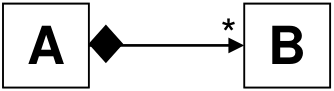
\includegraphics[width=1.0\textwidth]{figures/composite.png}
      \end{figure}
    \end{minipage}
    \begin{minipage}[t]{0.5\textwidth}
    \vspace{-3.5em}
    B is a fixed part of A that is:
    \begin{itemizenosep}
        \item B may be part of only one A
        \item If A is deleted, then also all its part
        \item Whole acts substitutions for all its parts\\
      $\Rightarrow$ operations are propagate to its parts
    \end{itemizenosep}
    \end{minipage}
  \end{defn}
\end{defnbox}
\begin{notebox}[Example]\nospacing
    House (parent) and a room (child), if we delete the house the
    room will be gone as well.
\end{notebox}
\begin{defnbox}\nospacing
  \begin{defn}[Aggregate]\label{defn:Aggregate}\leavevmode
    \begin{minipage}[t]{0.45\textwidth}
      \begin{figure}[H]
        \centering
        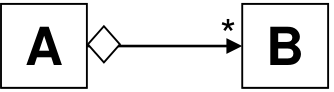
\includegraphics[width=1.0\textwidth]{figures/aggregate.png}
      \end{figure}
    \end{minipage}
    \begin{minipage}[t]{0.5\textwidth}
    \vspace{-3.5em}
    B is a variable part of A that is:
    \begin{itemizenosep}
        \item B may be part of several A's
        \item B may exist individually
    \end{itemizenosep}
    \end{minipage}
  \end{defn}
\end{defnbox}
\begin{notebox}[Example]\nospacing
    Class (parent) and Student (child), if we delete the class the
    students wills still exists, plus a student can be part of multiple classes.
\end{notebox}
\begin{figure}[H]
  \centering
  \vspace{-1em}
  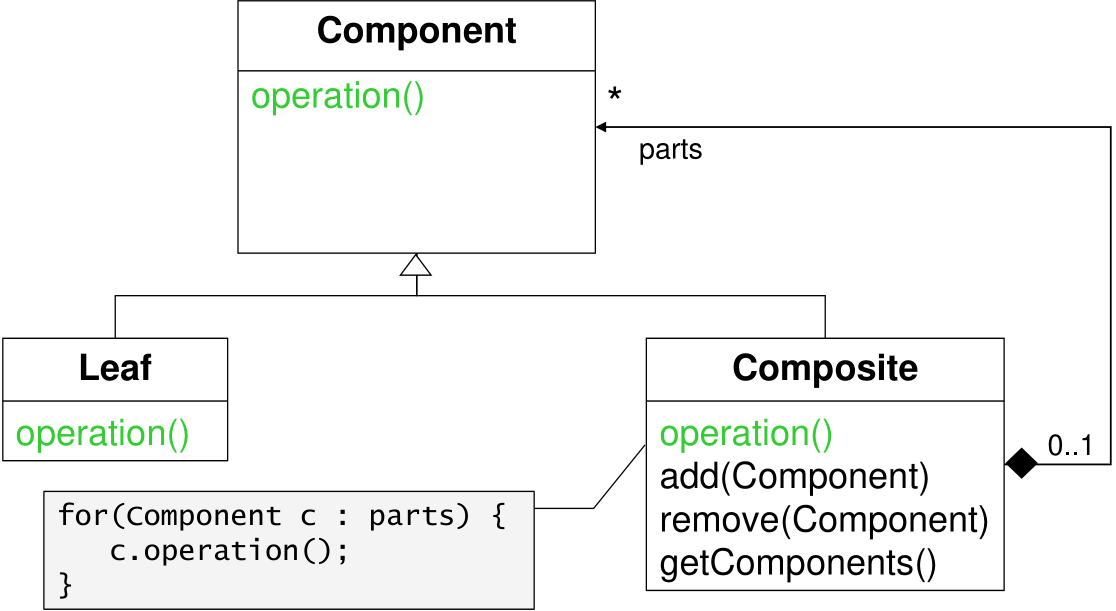
\includegraphics[width=1.0\columnwidth]{figures/compositePattern.png}
\end{figure}
\begin{intentbox}[Intent]
  Represent single/primitive components as hierarchical group such that we can treat
  the group object/composite the same way as the single objects.\\
  \imp{Examples} of operations applied uniformly on composites and single objects:
  \begin{itemize}
      \item Jdraw: move, draw, resize, copy
      \item File sizes: getSize, setProperties, delet
  \end{itemize}
\end{intentbox}
\begin{partbox}[Paticipants]
  \begin{itemizenosep}
      \item \imp{Abstract Class/Interface Component}: declares the base class
    and uniform methods implemented by the leaf primitives\\
      \imp{E.g.}\ Figure, Graphic, Shape, Room, ArithmeticOperation
      \item \imp{Leaves/primitives}: implements the Component interface/base class and
    specifies the behavior of the concrete primitive types\\
      \imp{E.g.}\ Rectangle, Text, Circle, PlayRoom, Multiply
      \item \imp{Composite}: implements the Component interface/base class and
      \begin{itemizenosep}
          \item Stores references to children which may be
          \begin{itemize}
              \item Leaves/Primitives
              \item Again composites
          \end{itemize}
          \item Implements methods to manage children add, remove, get
          \item Defines behavior of components containing children and must be
          concurrent with behavior of single elements
      \end{itemizenosep}
      \imp{E.g.} FigureGroup, GraphicsComposite, House,\\ ArithmeticExpression
        \item Client: manipulates objects through the Component interface
  \end{itemizenosep}
\end{partbox}
\subsection*{Transparent vs. Safe}
\label{subsubsec:TransparentVsSafe}
\begin{sectionbox}[Question]\nospacing
  Where should we \text{declare} the methods for managing the children, add, remove,\ldots?
  \begin{itemizenosep}
      \item \rdb{Transparent Approach}: declare them inside the Component
    interface
      \item \imp{\tc{Blue}{Safe Approach}}: declare them only inside the Composite
  \end{itemizenosep}
  \begin{figure}[H]
    \centering
    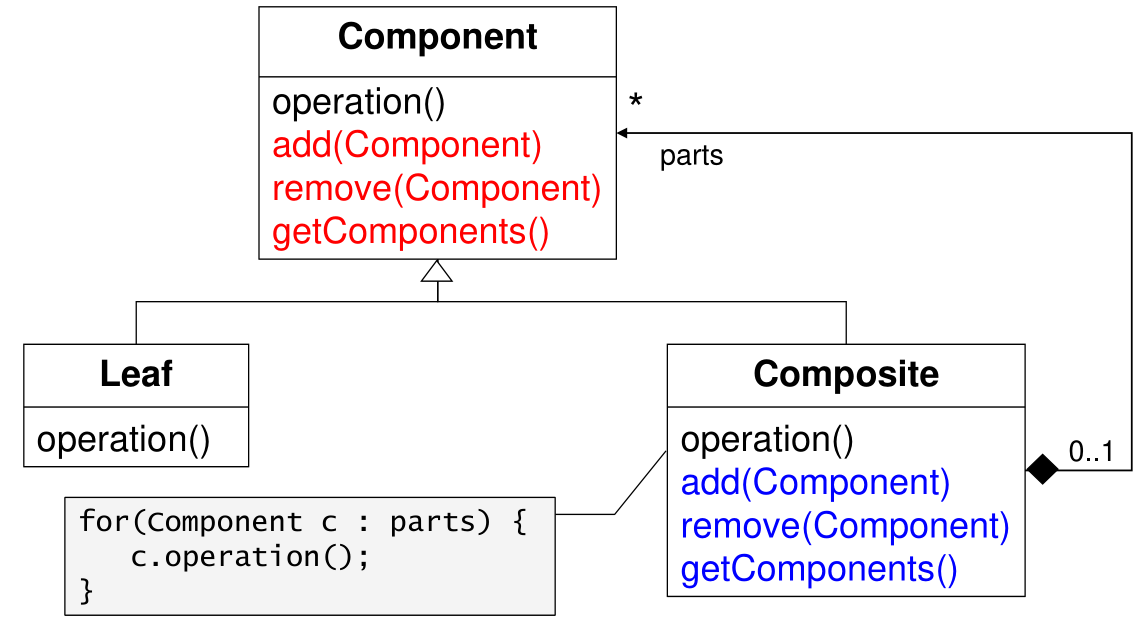
\includegraphics[width=1.0\textwidth]{figures/transSafe.png}
  \end{figure}
\end{sectionbox}
\subsubsection{\tc{Red}{Safe Approach \blackrb{Composite}}}
\begin{sectionbox}\nospacing
 Clients cannot do stupid/meaningless things s.a.\ adding, removing,\ldots from
 primitives/leaf objects because they do not even implement those methods
 $\Rightarrow$ compile time warning.
\end{sectionbox}
\todo[inline]{Understand what the drawback is with cast and treating uniformly}
\subsubsection{\tc{Blue}{Transparent Approach \blackrb{Component}}}
\begin{sectionbox}\nospacing
  Is the desire to treat composites and primitives uniformly/the same
  way/atomically/transparent and requires that we declare the child managing
  function inside the Component $\Rightarrow$ also the primitives must implement
  them $\Rightarrow$ clients may possibly do stupid things like adding to
  primitives.
\end{sectionbox}
\begin{sectionbox}[Solution 1]\nospacing
  Child managing methods inside the primitive throw an
  UnsupportedOperationException.\\
  \imp{Drawbacks}:
  \begin{itemizenosep}
      \item Program flow should not be controlled with exceptions
      \item Only transparent on the interface level
  \end{itemizenosep}
\end{sectionbox}
\begin{codeboxNl}{java}
  public void add|\optc{/}|remove(Component c ){
    throw new UnsupportedOperationException();
  }
 
  public void getComponents(){
    throw new UnsupportedOperationException();
  }
\end{codeboxNl}
\begin{sectionbox}[Solution 2]\nospacing
  Methods return a \javainline{boolean} result which informs the client whether
  the operation was successful.\\
  For \javainline{getComponents()} we can use
  \javainline{getComponents().getSize()} to check whether the composite contains
  components or not.
\end{sectionbox}
\begin{codeboxNl}{java}
  public boolean add(Component c) { return false; }
  public boolean remove(Component c) { return false; }
  public List getComponents() {return Collections.EMPTY_LIST;}
\end{codeboxNl}
\begin{sectionbox}[Solution 3]\nospacing
Method \javainline{isComposite} can be used to check whether a component is a
composite or not.\\
$\Rightarrow$ \javainline{isComposite()} should be called as precondition to
check if component is a composite, before add/remove,\ldots
\end{sectionbox}
\begin{codeboxNl}{java}
  public boolean isComposite() { return false; }
  public void add(Component c) { throw new AssertionError(); }
  public void remove(Component c){throw new AssertionError();}
  public List getComponents() {return Collections.EMPTY_LIST;}
\end{codeboxNl}
\begin{sectionbox}[Solution 4]\nospacing
  Default behavior is that nothing is done
\end{sectionbox}
\begin{codeboxNl}{java}
  public void add(Component c) {    /* do nothing */ }
  public void remove(Component c) { /* do nothing */ }
  public List getComponents() {return Collections.EMTPY_LIST;}
\end{codeboxNl}
\begin{sectionbox}[Solution 5]\nospacing
  Implement full functionality, that primitives can add and remove,\ldots
\end{sectionbox}
\subsection{Issues}
\begin{codeboxNl}[0..1 Constraint]{java}
  Figure f1 = new RectangleFigure(|\optldots|);
  Figure f2 = new RectangleFigure(|\optldots|);
  Figure f3 = new OvalFigure(|\optldots|);

  GroupFigure g1 = new GroupFigure(|\ul{f1}|, f2);
  GroupFigure g2 = new GroupFigure(f3, |\ul{f1}|);
\end{codeboxNl}
\begin{codeboxNl}[0..1 Constraint]{java}
  Figure f1 = new RectangleFigure(|\optldots|);
  Figure f2 = new RectangleFigure(|\optldots|);
  Figure f3 = new OvalFigure(|\optldots|);

  GroupFigure |\ul[ulc2]{g1}| = new GroupFigure(f1, f2);
  GroupFigure |\ul[ulc3]{g2}| = new GroupFigure(|\ul[ulc2]{g1}|, f3);

  |\ul[ulc2]{g1}|.addFigure(|\ul[ulc3]{g2}|);  // recursion
\end{codeboxNl}
\begin{sectionbox}[Solutions]\nospacing
  There exists to solutions:
  \begin{itemizenosep}
      \item \imp{Variant 1}: Only add component if it does not belong to anything:\\
      Check first for 0..1 constraint and then for recursion
      \item \imp{Variant 2}: If component belongs already to a composite remove it
      from current parent and add it to this composite.\\
      Check first for \ul[ulc4]{recursion} and then for 0..1 constraint
  \end{itemizenosep}
  in order to do this components need to have a parent field in order to check
  for recursions:
  \begin{mintlinebox}{java}
		Component parent;
  \end{mintlinebox}
\end{sectionbox}
\begin{codeboxNl}[Variant 1]{java}
void add(Component c) {
  // 1. Check 0..1 constraint
  if(c.parent != null) {
    throw new IllegalArgumentException("constraint violation");
  }
  // => c is for sure not part of anything
  // But c maybe composite itself 

  // 2. Check for recursion 
  // c has no parents => only possibility for recursion if
  // c is the same as root of this
  if(c instanceof Composite) {
    Composite comp = this;
    while (|\uldotted{comp.parent != null}|) { comp = comp.parent; }
    if(comp == c) {
      throw new IllegalArgumentException("recursion");
    }
  }

  c.parent = this;
  this.children.add(c);
}
\end{codeboxNl}
\begin{notebox}[Note]\nospacing
  Recursion only possible if \javainline{c} is the same as
  root of \javainline{this}. Root because we already know that
  \uldotted{\javainline{c} has not parent}.
\end{notebox}
\begin{codeboxNl}[Variant 2]{java}
void add(Component c) {
  // 1. Check for recursion
  // recursion not possible if c is primitive
  if(c instanceof Composite) {
    Composite comp = this;
    while (comp != null && comp != c) { comp = comp.parent; }
    // |go up in the hierarchy check for recursion
      if(|\ul[ulc4]{comp == c}|) {
        throw new IllegalArgumentException("recursion");
      }
    }

  // 2. Establish 0..1 constraint
  if(c.parent != null) {
    c.parent.remove(c);
  }

  c.parent = this;
  this.children.add(c);
}
\end{codeboxNl}
%%% Local Variables:
%%% mode: latex
%%% TeX-master: "../formulary"
%%% End:

\todo[inline]{MVC\&Callback lecture 7}
\subsection{Prototype Pattern}
\label{subsubsec:PrototypePattern}
\begin{figure}[H]	
  \centering
    \resizebox{\linewidth}{!}{\tikzset{font=\Huge}\documentclass{standalone}
\usepackage{tikz}
\usepackage{aeguill}
\begin{document}
% generated by Plantuml 1.2018.12      
\definecolor{plantucolor0000}{RGB}{254,254,206}
\definecolor{plantucolor0001}{RGB}{168,0,54}
\definecolor{plantucolor0002}{RGB}{173,209,178}
\definecolor{plantucolor0003}{RGB}{0,0,0}
\definecolor{plantucolor0004}{RGB}{169,220,223}
\begin{tikzpicture}[yscale=-1
,pstyle0/.style={color=plantucolor0001,fill=plantucolor0000,line width=1.5pt}
,pstyle1/.style={color=plantucolor0001,fill=plantucolor0002,line width=1.0pt}
,pstyle2/.style={color=plantucolor0001,line width=1.5pt}
,pstyle4/.style={color=plantucolor0001,line width=1.0pt}
]
\draw[pstyle0] (6pt,14.5pt) rectangle (81.7514pt,62.5pt);
\draw[pstyle1] (21pt,30.5pt) ellipse (11pt and 11pt);
\node at (21pt,30.5pt)[]{\textbf{\Large C}};
\node at (35pt,23.5156pt)[below right,color=black]{Client};
\draw[pstyle2] (7pt,46.5pt) -- (80.7514pt,46.5pt);
\draw[pstyle2] (7pt,54.5pt) -- (80.7514pt,54.5pt);
\draw[pstyle0] (167pt,8pt) rectangle (267pt,68.8047pt);
\draw[color=plantucolor0001,fill=plantucolor0004,line width=1.0pt] (182pt,24pt) ellipse (11pt and 11pt);
\node at (182pt,24pt)[]{\textbf{\Large A}};
\node at (196pt,17.0156pt)[below right,color=black]{\textit{Prototype}};
\draw[pstyle2] (168pt,40pt) -- (266pt,40pt);
\draw[pstyle2] (168pt,48pt) -- (266pt,48pt);
\node at (173pt,52pt)[below right,color=black]{\textit{createClone()}};
\draw[pstyle0] (25pt,130pt) rectangle (199.2194pt,190.8047pt);
\draw[pstyle1] (40pt,146pt) ellipse (11pt and 11pt);
\node at (40pt,146pt)[]{\textbf{\Large C}};
\node at (54pt,139.0156pt)[below right,color=black]{ConcretePrototype1};
\draw[pstyle2] (26pt,162pt) -- (198.2194pt,162pt);
\draw[pstyle2] (26pt,170pt) -- (198.2194pt,170pt);
\node at (31pt,174pt)[below right,color=black]{createClone()};
\draw[pstyle0] (234pt,130pt) rectangle (408.2194pt,190.8047pt);
\draw[pstyle1] (249pt,146pt) ellipse (11pt and 11pt);
\node at (249pt,146pt)[]{\textbf{\Large C}};
\node at (263pt,139.0156pt)[below right,color=black]{ConcretePrototype2};
\draw[pstyle2] (235pt,162pt) -- (407.2194pt,162pt);
\draw[pstyle2] (235pt,170pt) -- (407.2194pt,170pt);
\node at (240pt,174pt)[below right,color=black]{createClone()};
\draw[pstyle4] (82.3943pt,38.5pt) ..controls (105.7252pt,38.5pt) and (135.9024pt,38.5pt) .. (161.7689pt,38.5pt);
\draw[color=plantucolor0001,fill=plantucolor0001,line width=1.0pt] (166.8814pt,38.5pt) -- (157.8814pt,34.5pt) -- (161.8814pt,38.5pt) -- (157.8814pt,42.5pt) -- (166.8814pt,38.5pt) -- cycle;
\node at (100.5pt,19.5pt)[below right,color=black]{Uses};
\draw[color=black,fill=black,line width=1.0pt] (138.8333pt,25.5664pt) -- (144.8333pt,28.5664pt) -- (138.8333pt,31.5664pt) -- (138.8333pt,25.5664pt) -- cycle;
\draw[pstyle4] (177.0769pt,84.8868pt) ..controls (164.1654pt,99.8888pt) and (150.1755pt,116.1437pt) .. (138.4875pt,129.7241pt);
\draw[pstyle4] (172.1519pt,79.8783pt) -- (190.5041pt,69.2858pt) -- (182.7631pt,89.0108pt) -- (172.1519pt,79.8783pt) -- cycle;
\draw[pstyle4] (256.5429pt,84.8868pt) ..controls (269.3314pt,99.8888pt) and (283.188pt,116.1437pt) .. (294.7648pt,129.7241pt);
\draw[pstyle4] (250.8912pt,89.0472pt) -- (243.2436pt,69.2858pt) -- (261.5454pt,79.9649pt) -- (250.8912pt,89.0472pt) -- cycle;
\end{tikzpicture}
\end{document}
}
\end{figure}
\subsection{Comparing Objects}
\begin{defnbox}\nospacing
  \begin{defn}[\javainline{obj1==obj2}]
    Compares references/addresses of the two operands.\\
  \end{defn}
\end{defnbox}
\begin{defnbox}\nospacing
  \begin{defn}[\javainline{obj1.equals(obj2)}]
    Compares the content of two objects.
  \end{defn}
\end{defnbox}
\begin{defnbox}\nospacing
  \begin{defn}[\javainline{obj1.getClass()==obj2.getClass()}]\label{defn:}
    Checks if two objects are of the same \rd{dynamic} type.
  \end{defn}
\end{defnbox}
\begin{defnbox}\nospacing
  \begin{defn}[\javainline{obj is instanceof}]
    Checks if an object is an instance of a class or interface.
  \end{defn}
\end{defnbox}
\begin{intentbox}[Intent of cloning]
  Provide a clone that satisfies:
  \begin{itemizenosep}
      \item New instance: \javainline{x.clone()!=x}
      \item Same dynamic type: \javainline{x.clone().getClass()==x.getClass()}
      \item Equal: \javainline{x.clone().equals(x)}
  \end{itemizenosep}
\end{intentbox}
\subsection{Deep vs. Shallow Copies}
\begin{figure}[H]
  \centering
  \vspace{-1em}
  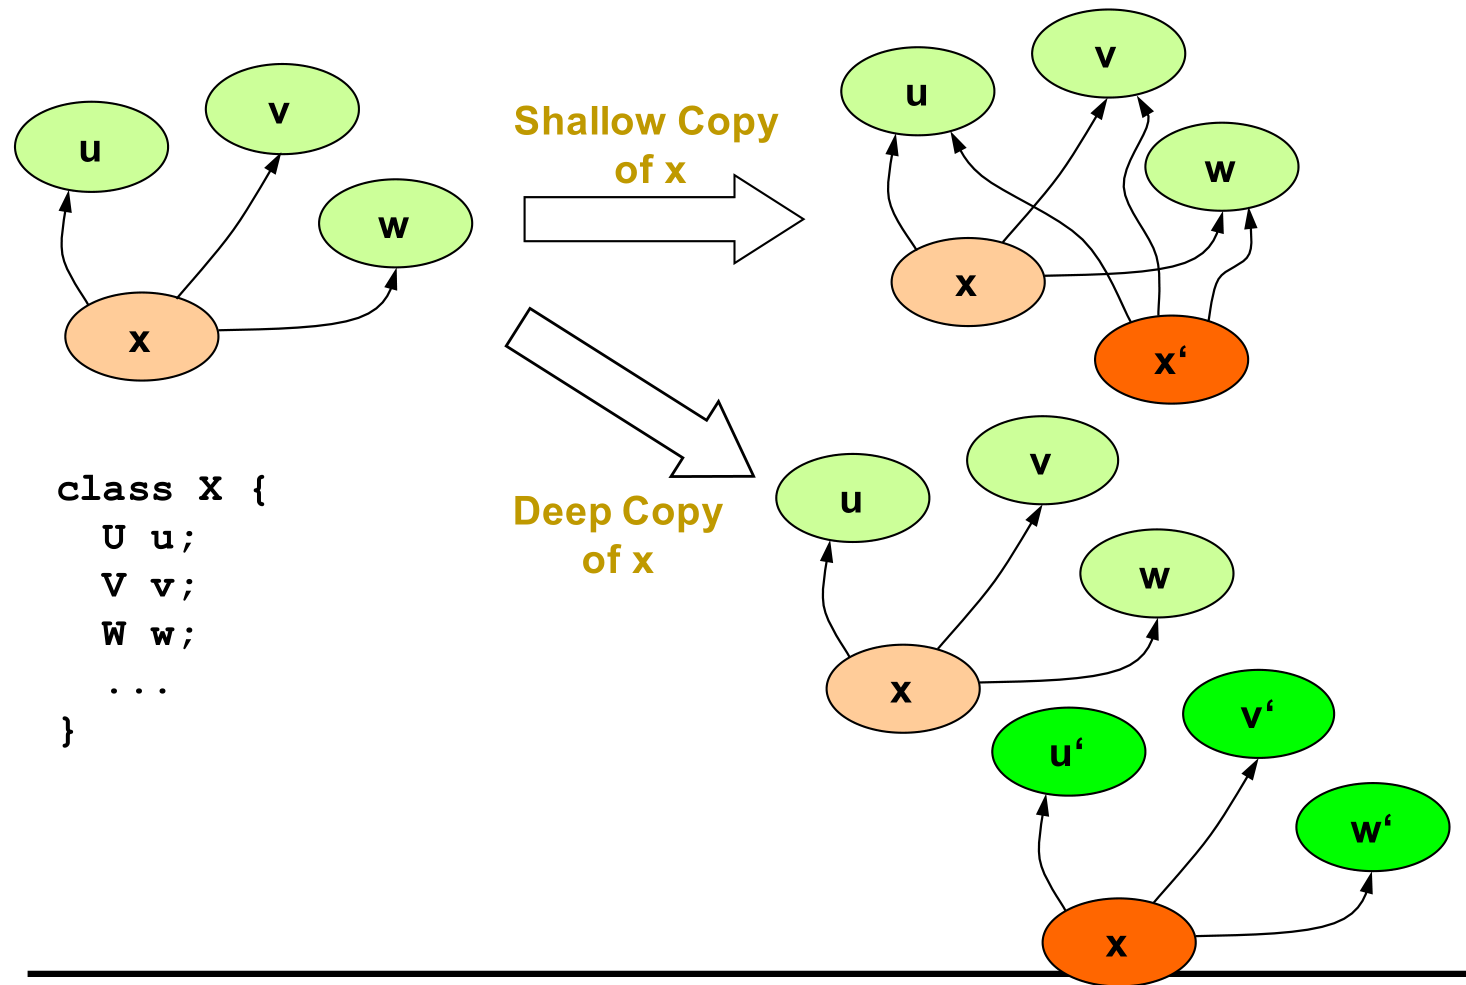
\includegraphics[width=1.0\columnwidth]{figures/shallowVsDeppCopy.png}
\end{figure}
\begin{defnbox}\nospacing
  \begin{defn}[Shallow Copy]\label{defn:shallowCopy}
    Is a bit-wise copy of an object. A new object is created that has an exact
    copy of the values in the original object.\\
    \imp{Thus}: If any of the fields of the object are references to other
    mutable types/objects, just the reference addresses are copied i.e., only
    the memory address is copied.\\
    \begin{mintlinebox}{java}
      myFoo.childObj == sFoo.childObj // ture
      myFoo.childObj.equals(sFoo.childObj) // ture
    \end{mintlinebox}
    \imp{Hence} manipulating child mutable types/objects of the copy will also modify the child mutable types/objects
    of the original object $\Rightarrow$ not a real copy.
  \end{defn}
\end{defnbox}
\begin{notebox}[Attention]\nospacing
  Lists are complex types!
\end{notebox}
\begin{codeboxNl}[Shallow list copy]{java}
  public class Ex { 
    private int[] data; 
    // makes a shallow copy of values 
    public Ex(int[] values) { 
        data = values; 
    } 
} 
\end{codeboxNl}
\begin{defnbox}\nospacing
  \begin{defn}[Deep copy]\label{defn:deepcopy}
    Recursively copies objects, and hence is a real copy.
    \begin{mintlinebox}{java}
      myFoo.childObj == sFoo.childObj // false
      myFoo.childObj.equals(sFoo.childObj) // ture
    \end{mintlinebox}
  \end{defn}
\end{defnbox}
\begin{codeboxNl}{java}
class Foo {
  private Bar myBar;
  ...
  public Foo shallowCopy() {
    Foo newFoo = new Foo();
    newFoo.myBar = myBar;
    return newFoo;
  }

  public Foo deepCopy() {
    Foo newFoo = new Foo();
    newFoo.myBar = myBar.clone();
    return newFoo;
  }
}

Foo myFoo = new Foo();  
Foo sFoo = myFoo.shallowCopy();  
Foo dFoo = myFoo.deepCopy();  

myFoo.myBar == sFoo.myBar => true  
myFoo.myBar.equals(sFoo.myBar) => true  
myFoo.myBar == dFoo.myBar => **false**  
myFoo.myBar.equals(dFoo.myBar) => true  
\end{codeboxNl}
\subsubsection{Java.lang.Clonable}
\label{subsubsec:Java.lang.Clonable}
\begin{defnbox}\nospacing
  \begin{defn}[Clonable]\label{defn:}
    Is a marker interface \cref{defn:markerInerface}, that is special in that
    it is empty and does not even declare the clone method:
    \begin{mintlinebox}{java}
      public interface Cloneable {
        // Marker interface
      }
    \end{mintlinebox}
    It is simply there to indicate that a class is clonable.
  \end{defn}
\end{defnbox}
\begin{codeboxNl}[java.lang.Object]{java}
protected Object clone() throws CloneNotSupportedException {
  if (!(this instanceof Cloneable)) {
    throw new CloneNotSupportedException(
      "Doesn't implement Cloneable interface!");
  }
  return VMMemoryManager.clone(this);
}
\end{codeboxNl}
\begin{codeboxNl}[VMMemoryManager]{java}
  class VMMemoryManager {
    static native Object clone(Object object);
    |\ldots|
  }
\end{codeboxNl}
\begin{defnbox}\nospacing
  \begin{defn}[\javainline{nativ}]
    Enables java code running JVM to call\& be called by nativ applications
    (programs specific to hardware\&OS platform) and libraries written in other
    languages e.g.\ C.\\
    \imp{Here}: it calls C-code that uses \cppinline/memcpy/ to
    copy the given object \rd{bitwise} efficiently ($\Rightarrow$ \rd{shallow copy}).
  \end{defn}
\end{defnbox}
\subsubsection{Java.lang.Object and Clonable}
\begin{defnbox}\nospacing
  \begin{defn}[Java.lang.Object]\label{defn:}
    Is the base class of all Classes and provides a \javainline{protected}
    default implementation of the \javainline{clone} method which:
    \begin{itemizenosep}
      \item Throws an \javainline{CloneNotSupportedException}
      if an object of a class calls the clone method without
      implementing the \javainline{Cloneable} marker interface
      \item Will lead to a compile time error if we try to copy an object
      not from within itself, subclasses, or classes of the same package.\\
      This is because clone is \javainline{protected}
    \end{itemizenosep}
  \end{defn}
\end{defnbox}
\begin{defnbox}[How to use:]\nospacing
    \javainline{java.lang.Object.clone} the right way:
    \begin{itemizenosep}
        \item If the Class we want to clone only contains primitive fields or
      references to \javainline{immutable} objects, then we can simply:\\
      \rdb{Shallow Copy}:
      \begin{itemize}
          \item override the \javainline{clone} method as a public method
          \item call \javainline{super.clone()} to make a shallow copy using \cppinline/memcpy/
      \end{itemize}
      \begin{mintlinebox}{java}
        |\optc{visibility}| class MyClass implements Cloneable{
          |\optldots|
          public Object clone(){
            |\ul[ulc2]{try}|{
              // go up in hierarchy until
              // java.lang.Object.clone
              MyClass c = |\ul{(MyClass)}| super.clone();
              return c;
            } catch (CloneNotSupportedException e){
              throw new InternalError(e.getMessage());
            }
          }
        }
      \end{mintlinebox}
    \end{itemizenosep}
\end{defnbox}
\begin{notebox}[Notes]\nospacing
  \begin{itemizenosep}
      \item \ul{Type Conversion}: MyClass may be a subclass of another class
    i.e.\ the parent class will call again \javainline{super.clone} until
    we reach \javainline{java.lang.object}.\\
    Hence we need to make sure that we will obtain the right dynamic type
    (\javainline{x.clone().getClass()==x.getClass()}).
      \item \ul[ulc2]{try}: again if MyClass is a subclass of other, the
      super/parent classes need to implement at least the \javainline{clonable}
      marker interface (do not necessarily need to implement clone method).
  \end{itemizenosep}
\end{notebox}
\begin{defnbox}\nospacing
  \begin{itemizenosep}
    \item If the Class we want to clone does contains complex fields or
    references to \javainline{mutable} types then we need to:\\
      \rdb{Deeply Copy}:
    \begin{itemize}
        \item Recursively clone all elements
        \item Replace lists with new ones
    \end{itemize}
  \end{itemizenosep}
\end{defnbox}
\begin{codeboxNl}[Company: Deep Copy]{java}
public class Company implements Cloneable {
  private String name;
  // Java lists are mutable data types!
  private ArrayList<Employee> employees = new ArrayList<>();
  public Object clone() {
    try {
      Company c = (Company) super.clone();
      c.employees = new ArrayList<>();
      for(Employee e : employees)     
        c.employees.add(e.clone());
      return c;
    } catch (CloneNotSupportedException e) {
      throw new InternalError(e.getMessage());
    }
  }     
}
\end{codeboxNl}
\begin{codeboxNl}[Employee: Shallow Copy]{java}
public class Employee implements Cloneable {
  // Only primitive types
  private String name;
  private int yearOfBirth;
  public Object clone() {
    try {
      return super.clone();
    } catch (CloneNotSupportedException e) {
      throw new InternalError(e.getMessage());
    }
  }
}
\end{codeboxNl}
\begin{notebox}[Why is clone protected?]\nospacing
  \begin{itemizenosep}
      \item 
  Clone is declared protected so that if all we do is implement Cloneable, only
  subclasses and members of the same package will be able to invoke clone() on
  the object.\\
  To enable any class in any package to access the clone() method, you'll have
  to override it and declare it \javainline{public}! 
      \item Clone cannot be invoked on objects of static type Object.
  \end{itemizenosep}
\end{notebox}
\begin{codeboxNl}[Compile Time Error]{java}
  import myClass
  // Implementing (empty) marker interface
  // But does not implement clone method

  class Client{
    public static void main(String[] args){
      myClass obj1 = new myClass();
      // Compile time error => calling protected method
      myClass obj2 = obj1.clone();
      
    }
  }
\end{codeboxNl}
\begin{notebox}[Notes]\nospacing
  \begin{itemizenosep}
      \item Java allows covariant typing \label{defn:covariantTying}
      \item Alias references and cycles have to be handled manually
  \end{itemizenosep}
\end{notebox}
\subsubsection{Clone with copy Constructor}
\begin{sectionbox}\nospacing
  Java does not provide a default copy constructor as in C++ but we may write
  one and then use it for our clone method.
\end{sectionbox}
\begin{codeboxNl}[Clone with copy constructor]{java}
class Company {
  public Company(Company c) {
    if(c==null) throw new IllegalArgumentException();
      // initialize this with attributes of c
    }
    |\optldots|
    public Company clone() {
      return new Company(this);
    }
}
\end{codeboxNl}
\begin{notebox}[Notes]\nospacing
  \begin{itemizenosep}
      \item It is possible that the state of an immutable type
       changes after creation, as long as this change is not visible to the
       client.
      \item Companion mutables: provide conversion classes e.g.\
    immutable \javainline{string} and mutable \javainline{stringBuffer}
  \end{itemizenosep}
  Provide conversionhh
\end{notebox}
\subsubsection{Prototype Design Pattern}
\begin{figure}[H]
  \centering
  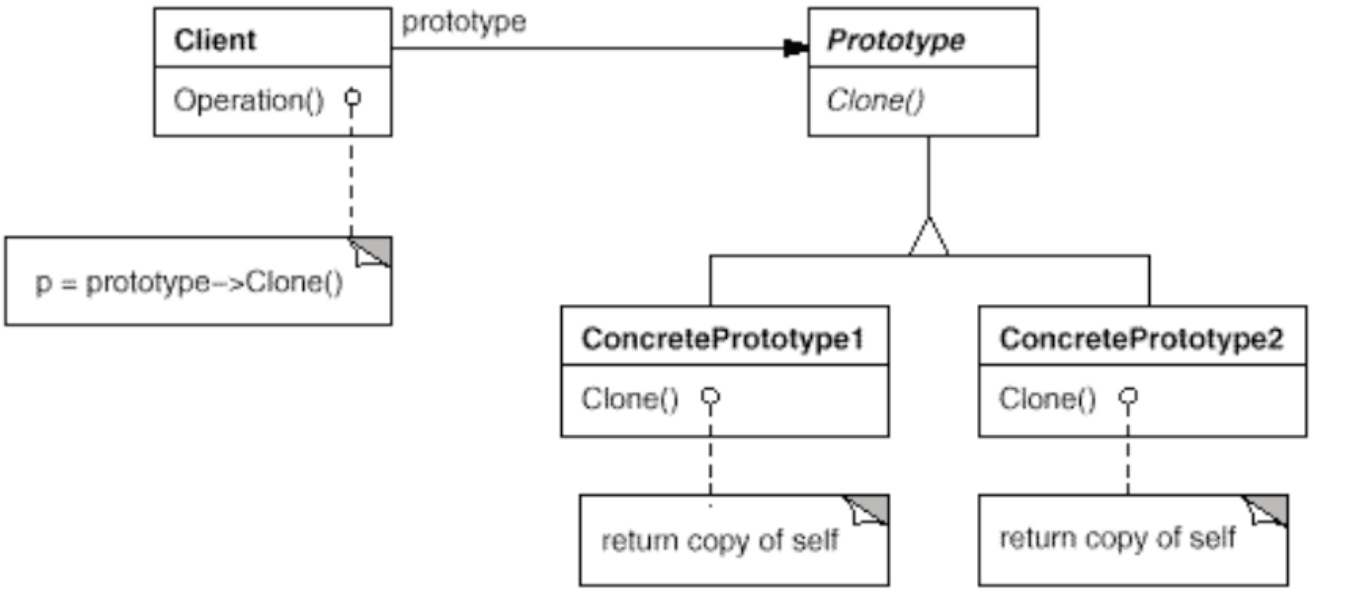
\includegraphics[width=1.0\columnwidth]{figures/prototypePattern.png}
\end{figure}
\begin{sectionbox}[Problem]\nospacing
  New object creation \javainline{MyClass obj = new MyClass()} is costly e.g.\
  an object is created by calling a costly database operation inside the constructor.\\
  Thus if we need many similar types it is not a good idea to always construct a
  new object using \javainline{new}.
\end{sectionbox}
\begin{intentbox}[Intent]
    Avoid costly creation of an object using \javainline{new} by \textit{cloning
      it from some similar prototype} and simply adapt it to our needs.\\
    \imp{Thus}: we specify the kinds of objects to create using a prototypical
    instance, and create new objects by cloning the right prototype.
\end{intentbox}
\begin{partbox}[Participants]
  \begin{itemizenosep}
      \item \imp{Prototype}:
      \item
      \begin{itemizenosep}
        \item Is in its easiest form the \javainline{java.lang.Clonable}
      interface
        \item An interface that implements the clonable interface
        \begin{itemize}
            \item Implements the clonable marker interface
            \item declares a public clone method
            \item may declare methods for other classes
        \end{itemize}
          \item An abstract class e.g.\ Shape implementing the
        \javainline{java.lang.Clonable} interface
      \end{itemizenosep}
        \item \imp{Concrete Prototype}: is an concrete class implementing the
      prototype interface that we may want to clone
        \item \imp{Client}: Produces new instances by calling clone on concrete
      prototypical prototypes.
  \end{itemizenosep}
\end{partbox}
\begin{notebox}[Note: Why not just use clonable interface]\nospacing
  Many consider clonable as broken/bad design as it does not even declare clone
  thus checking anything with the clonable marker interface does not bring us
  anything e.g.\
  \begin{mintlinebox}{java}
       concretPrototype a = new A();
       if(a instanceof Cloneable)
       {
         // This check is worthless and
         // the method may fail
           A copied = a.clone(); 
       }
  \end{mintlinebox}
\end{notebox}
\begin{codeboxNl}[Abstract Prototype]{java}
abstract class Prototype implements Cloneable {

  public Prototype clone() throws CloneNotSupportedException {
    return (Prototype) super.clone();
  }
  public abstract void setX(final shot X);
  public abstract short getX();
}
\end{codeboxNl}
\begin{codeboxNl}[Concrete Prototype]{java}
class ConcretePrototype implements Prototype {
  private int x;

  public ConcretePrototype extends Prototype {
    return (Prototype) super.clone();
  }

  public abstract void setX(int X){
    x = X;
  }

  public abstract short getX(){
    return x;
  }
}
\end{codeboxNl}
\begin{codeboxNl}[Client]{java}
public class Client{
  public static void main(String[] args) {
  Prototype origin =  new ConcretePrototype(10);
  Prototype clone =  origin.clone();
  clone.setX(4);
}
\end{codeboxNl}
\subsubsection{Exmple}
\label{subsubsec:Exmple}
\begin{codeboxNl}[Abstract Prototype]{java}
public abstract class Figure implements Cloneable {
  |\optldots|
  public Object clone() {
      Object clone = null;
      try {
         clone = super.clone();
      } catch (CloneNotSupportedException e) {
         e.printStackTrace();
      }
      return clone;
      // Or do not let clone abstract base class
    }
}
\end{codeboxNl}
\begin{codeboxNl}[Concrete Prototype]{java}
public class Rectangle extends Figure {
  |\optldots|
  public Object clone() {
      Object clone = null;
      try {
         clone = super.clone();
         // or provide deep copy
      } catch (CloneNotSupportedException e) {
         e.printStackTrace();
      }
      return clone;
    }
}
\end{codeboxNl}
\begin{codeboxNl}[Client]{java}
public class Client{
  |\optldots|
  Rectangle greenRec = new Rectangle(green);
  Circle blueCircle = new Circle(blue);
  Circle yellowCircle = new Circle(yellow);

  public static void main(String[] args) {
    Rectangle myRecClone = greenRec.clone();
    Circle myCircleClone = yellowCircle.clone();
  }
\end{codeboxNl}
%%% Local Variables:
%%% mode: latex
%%% TeX-master: "../formulary"
%%% End:

\subsection{Decorator Pattern}
\label{subsubsec:DecoratorPattern}
\begin{figure}[H]	
  \centering
    \resizebox{\linewidth}{!}{\tikzset{font=\Huge}\documentclass{standalone}
\usepackage{tikz}
\usepackage{aeguill}
\begin{document}
% generated by Plantuml 1.2018.12      
\definecolor{plantucolor0000}{RGB}{254,254,206}
\definecolor{plantucolor0001}{RGB}{168,0,54}
\definecolor{plantucolor0002}{RGB}{169,220,223}
\definecolor{plantucolor0003}{RGB}{0,0,0}
\definecolor{plantucolor0004}{RGB}{173,209,178}
\definecolor{plantucolor0005}{RGB}{255,255,255}
\begin{tikzpicture}[yscale=-1
,pstyle0/.style={color=plantucolor0001,fill=plantucolor0000,line width=1.5pt}
,pstyle2/.style={color=plantucolor0001,line width=1.5pt}
,pstyle3/.style={color=plantucolor0001,fill=plantucolor0004,line width=1.0pt}
,pstyle4/.style={color=plantucolor0001,line width=1.0pt}
]
\draw[pstyle0] (6pt,8pt) rectangle (118.2286pt,94.4141pt);
\draw[color=plantucolor0001,fill=plantucolor0002,line width=1.0pt] (21pt,24pt) ellipse (11pt and 11pt);
\node at (21pt,24pt)[]{\textbf{\Large A}};
\node at (35pt,17.0156pt)[below right,color=black]{\textit{Component}};
\draw[pstyle2] (7pt,40pt) -- (117.2286pt,40pt);
\draw[pstyle2] (7pt,48pt) -- (117.2286pt,48pt);
\node at (12pt,52pt)[below right,color=black]{\textit{method1()}};
\node at (12pt,64.8047pt)[below right,color=black]{\textit{method2()}};
\node at (12pt,77.6094pt)[below right,color=black]{\textit{method3()}};
\draw[pstyle0] (350pt,154pt) rectangle (527.9748pt,240.4141pt);
\draw[pstyle3] (365pt,170pt) ellipse (11pt and 11pt);
\node at (365pt,170pt)[]{\textbf{\Large C}};
\node at (379pt,163.0156pt)[below right,color=black]{ConcreteComponent};
\draw[pstyle2] (351pt,186pt) -- (526.9748pt,186pt);
\draw[pstyle2] (351pt,194pt) -- (526.9748pt,194pt);
\node at (356pt,198pt)[below right,color=black]{method1()};
\node at (356pt,210.8047pt)[below right,color=black]{method2()};
\node at (356pt,223.6094pt)[below right,color=black]{method3()};
\draw[pstyle0] (10.5pt,166.5pt) rectangle (113.3393pt,227.3047pt);
\draw[pstyle3] (25.5pt,182.5pt) ellipse (11pt and 11pt);
\node at (25.5pt,182.5pt)[]{\textbf{\Large C}};
\node at (39.5pt,175.5156pt)[below right,color=black]{Decorator};
\draw[pstyle2] (11.5pt,198.5pt) -- (112.3393pt,198.5pt);
\node at (16.5pt,202.5pt)[below right,color=black]{component};
\draw[pstyle2] (11.5pt,219.3047pt) -- (112.3393pt,219.3047pt);
\draw[pstyle0] (148.5pt,154pt) rectangle (315.9769pt,240.4141pt);
\draw[pstyle3] (163.5pt,170pt) ellipse (11pt and 11pt);
\node at (163.5pt,170pt)[]{\textbf{\Large C}};
\node at (177.5pt,163.0156pt)[below right,color=black]{ConcreteDecorator};
\draw[pstyle2] (149.5pt,186pt) -- (314.9769pt,186pt);
\draw[pstyle2] (149.5pt,194pt) -- (314.9769pt,194pt);
\node at (154.5pt,198pt)[below right,color=black]{method1()};
\node at (154.5pt,210.8047pt)[below right,color=black]{method2()};
\node at (154.5pt,223.6094pt)[below right,color=black]{method3()};
\draw[pstyle4] (137.2656pt,79.0956pt) ..controls (191.7443pt,99.5561pt) and (267.0767pt,128.1046pt) .. (333pt,154pt) ..controls (338.5453pt,156.1783pt) and (344.2466pt,158.4365pt) .. (349.9912pt,160.7261pt);
\draw[pstyle4] (134.4625pt,85.5205pt) -- (118.194pt,71.9434pt) -- (139.3785pt,72.412pt) -- (134.4625pt,85.5205pt) -- cycle;
\draw[pstyle4] (49.3526pt,114.2046pt) ..controls (48.972pt,132.2759pt) and (49.6503pt,151.1628pt) .. (51.3873pt,166.3269pt);
\draw[pstyle4] (42.3689pt,113.6812pt) -- (50.2585pt,94.0152pt) -- (56.3549pt,114.3089pt) -- (42.3689pt,113.6812pt) -- cycle;
\draw[pstyle4] (75.178pt,107.2226pt) ..controls (75.7719pt,122.4473pt) and (75.5442pt,138.7013pt) .. (74.4949pt,153.1368pt);
\draw[color=plantucolor0001,fill=white,line width=1.0pt] (73.237pt,166.3269pt) -- (77.7886pt,160.7338pt) -- (74.3763pt,154.3811pt) -- (69.8247pt,159.9742pt) -- (73.237pt,166.3269pt) -- cycle;
\draw[color=plantucolor0001,fill=plantucolor0001,line width=1.0pt] (74.4321pt,94.0152pt) -- (70.9459pt,103.2264pt) -- (74.714pt,99.0072pt) -- (78.9332pt,102.7753pt) -- (74.4321pt,94.0152pt) -- cycle;
\draw[pstyle4] (74.714pt,99.0072pt) -- (75.1652pt,106.9945pt);
\draw[pstyle4] (133.8172pt,197pt) ..controls (138.6871pt,197pt) and (143.5569pt,197pt) .. (148.4267pt,197pt);
\draw[pstyle4] (133.7969pt,203.9999pt) -- (113.7969pt,197pt) -- (133.7968pt,189.9999pt) -- (133.7969pt,203.9999pt) -- cycle;
\end{tikzpicture}
\end{document}
}
\end{figure}
\begin{intentbox}[Intent]
  We have some basic building blocks that share common method declarations
  but may have lots of different functionality.\\
  $\Rightarrow$ attach dynamically additional responsibility to an object by
  passing it to a decorator.
  \begin{figure}[H]
    \centering
    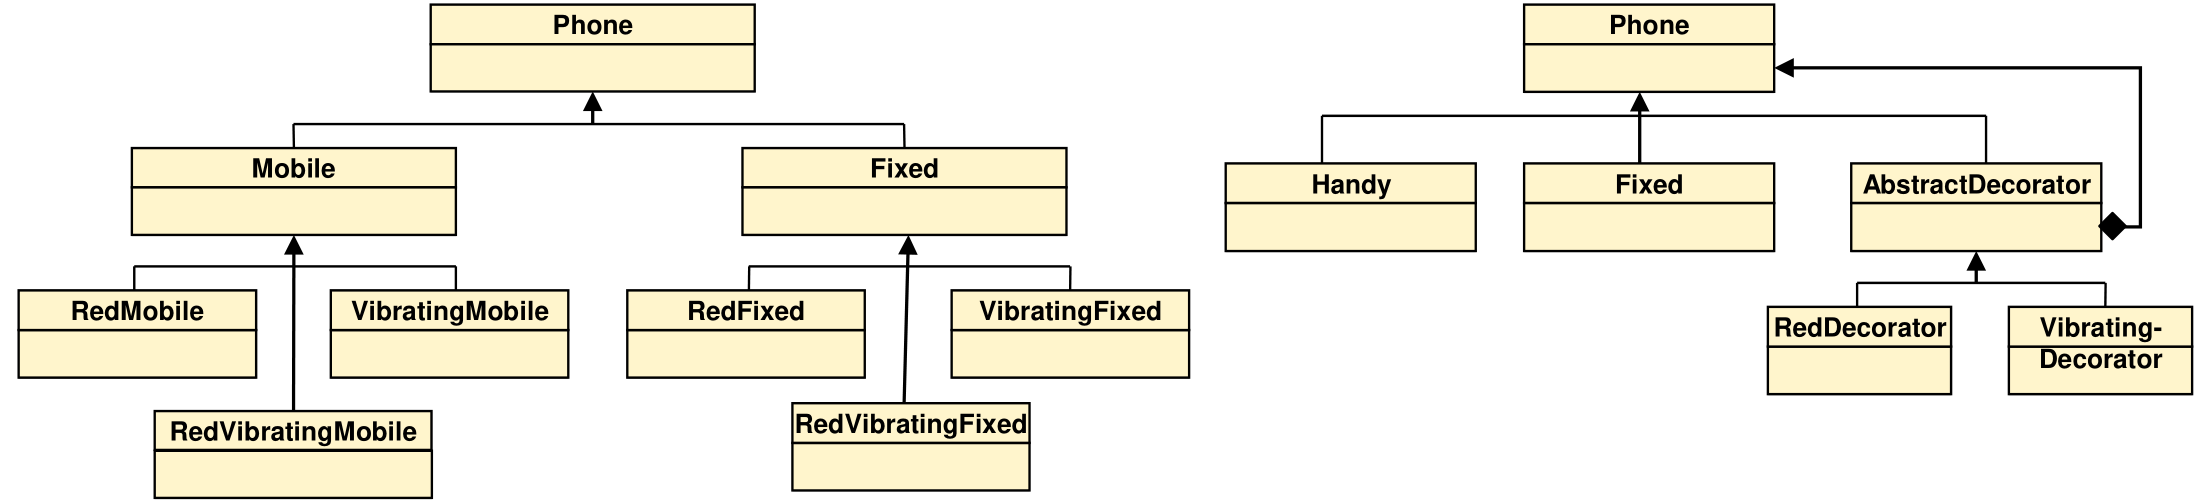
\includegraphics[width=1.0\textwidth]{figures/decoratorExplosion.png}
    \caption{Inheritance vs. Decoration}
    \vspace{-1em}
  \end{figure}
  \begin{align*}
    &n: \text{ number of properties}\\[-1\jot]
    &\text{\# of Subclasses with inheritance\&combination }&&2^n-1 \\[-1\jot]
    &\text{\# of additoinal Classes with decoration }&&n+1
  \end{align*}
\end{intentbox}
\begin{partbox}[Participants]
  \begin{itemizenosep}
    \item \imp{Basic building blocks}: is, or are they things that we want to
    decorate/add functionality to.
    \item \imp{Component Interface}: declares the shared methods of the basic
    building blocks that may be decorated by the decorator.\\
    The component interface is also implemented by the decorator.\\
    $\Rightarrow$ Leads to consistency between the decorator and the basic
    building blocks by declaring the methods that may be decorated.
    \item \imp{Decorator}: Is an \textit{optional}
    \begin{itemizenosep}
      \item abstract wrapper class that defines the shared methods and fields of
      the concrete decorators i.e.\ stores a reference to a basic building block
      or more commonly
        \item a wrapper class that
        \begin{itemize}
            \item stores a reference to the basic building block 
            \item simply calls the to be decorated methods of the reference to
          the building block
        \end{itemize}
    \end{itemizenosep}
      \item \imp{Client}: creates decorated classed by handing/decorating basic
      building blocks by decorators.
  \end{itemizenosep}
\end{partbox}
\begin{notebox}[Note]\nospacing
  A concrete Decorator class is useful if concreteDecorators do not decorate
  all methods that may possibly decorated!
\end{notebox}
\begin{codeboxNl}[Component e.g.\ Figure]{java}
  interface Component{
    public |\optc{type}| op1(|\optc{args}|);    // e.g. draw
    public |\optc{type}| op2(|\optc{args}|);    // e.g. setBounds
  }
\end{codeboxNl}
\begin{codeboxNl}[Concrete Component/Basic Building Block e.g.\ Rectangle]{java}
  class concreteCompA implements Component{
    public |\optc{type}| op1(|\optc{args}|){
        |\\optc{do something1}|
    };
    public |\optc{type}| op2(|\optc{args}|){
        |\optc{do something2}|
    }
  }
\end{codeboxNl}
\begin{codeboxNl}[Decorator]{java}
class Decorator implements Component{
  Component inner;
  public Decorator(Component inner){
    this.inner = inner;
  }
  // No decoration yet
  public |\optc{type}| op1(|\optc{args}|){
    inner.op1(|\optc{args}|);
  }

  public |\optc{type}| op2(|\optc{args}|){
    inner.op2(|\optc{args}|);
  }
}
\end{codeboxNl}
\begin{codeboxNl}[ConcreteDecorator e.g.\ ColorDecorator]{java}
class op1Decorator extends Decorator{
  @override
  public |\optc{type}| op1(|\optc{args}|){
    // Decorate before
    inner.op1(|\optc{args}|);
    // Decorate after
    addFunctionality(|\optc{args}|);
  }

  public |\optc{type}| addFunctionality(|\optc{args}|){
    // Do something
  }
}
\end{codeboxNl}
\begin{notebox}[Note]\nospacing
  \javainline{inner} may very well be another \javainline{concreteDecorator}
  and not a basic building block.
\end{notebox}
\begin{codeboxNl}[Client]{java}
  Oval ov = new Oval();
  RedColorDecorator redRec = new RedColorDecorator(ov);
\end{codeboxNl}
\begin{codeboxNl}[Client Example 2]{java}
  // MobilePhone implements Phone and has methods vibration and color
  MobilePhone m = new MobilePhone();
  RedColorDecorator redRec = new RedColorDecorator(ov);
  Phone redVibratingPhone =
          new RedColorDecorator(new VibrationDecorator(m));
\end{codeboxNl}
\begin{notebox}[Notes]\nospacing
  \begin{itemizenosep}
      \item May apply decorator before or after e.g.\
      may use decorator for some type safety checking
      \item 
  May also make sense to pass inner to setter method.
  \end{itemizenosep}
\end{notebox}
\subsubsection{Fields}
\label{subsubsec:Fields}
\begin{sectionbox}\nospacing
 Fields cannot be decorated explicitly \imp{but} if the basic building blocks
 use \javainline{getters} and \javainline{setters} then we may decorate them
 implicitly via those methods.
\end{sectionbox}
\begin{notebox}[Decorator vs State vs Strategy]\nospacing
  \begin{itemizenosep}
      \item A \tc{section}{Decorator} changes an object’s skin: that is it
    usually adds functionality (decorates) e.g.\ DrawTools may be decorators of
    the view.
      \item A \tc{section}{Strategy} changes an object’s guts: that is it is
      likely to change the internal strategy
      \item \tc{section}{State} changes an object’s guts: that is it is
      likely to changed its functionality completely 
  \end{itemizenosep}
\end{notebox}
\todo[inline]{Add type tests and problems (rest of slids)}
%%% Local Variables:
%%% mode: latex
%%% TeX-master: "../formulary"
%%% End:

\subsection{Proxy Pattern}
\label{subsubsec:ProxyPattern}
\begin{defnbox}\nospacing
  \begin{defn}[Proxy]
     Latin word meaning ``the authority to represent someone else''.
  \end{defn}
\end{defnbox}
\begin{figure}[H]	
  \centering
    \resizebox{\linewidth}{!}{\tikzset{font=\Huge}\documentclass{standalone}
\usepackage{tikz}
\usepackage{aeguill}
\begin{document}
% generated by Plantuml 1.2018.12      
\definecolor{plantucolor0000}{RGB}{254,254,206}
\definecolor{plantucolor0001}{RGB}{168,0,54}
\definecolor{plantucolor0002}{RGB}{173,209,178}
\definecolor{plantucolor0003}{RGB}{0,0,0}
\definecolor{plantucolor0004}{RGB}{180,167,229}
\definecolor{plantucolor0005}{RGB}{255,255,255}
\begin{tikzpicture}[yscale=-1
,pstyle0/.style={color=plantucolor0001,fill=plantucolor0000,line width=1.5pt}
,pstyle1/.style={color=plantucolor0001,fill=plantucolor0002,line width=1.0pt}
,pstyle2/.style={color=plantucolor0001,line width=1.5pt}
,pstyle4/.style={color=plantucolor0001,line width=1.0pt}
,pstyle5/.style={color=plantucolor0001,fill=plantucolor0001,line width=1.0pt}
,pstyle6/.style={color=plantucolor0001,fill=white,line width=1.0pt}
,pstyle7/.style={color=black,fill=black,line width=1.0pt}
]
\draw[pstyle0] (6pt,27pt) rectangle (81.7514pt,75pt);
\draw[pstyle1] (21pt,43pt) ellipse (11pt and 11pt);
\node at (21pt,43pt)[]{\textbf{\Large C}};
\node at (35pt,36.0156pt)[below right,color=black]{Client};
\draw[pstyle2] (7pt,59pt) -- (80.7514pt,59pt);
\draw[pstyle2] (7pt,67pt) -- (80.7514pt,67pt);
\draw[pstyle0] (166.5pt,8pt) rectangle (251.9213pt,94.4141pt);
\draw[color=plantucolor0001,fill=plantucolor0004,line width=1.0pt] (181.5pt,24pt) ellipse (11pt and 11pt);
\node at (181.5pt,24pt)[]{\textbf{\Large I}};
\node at (195.5pt,17.0156pt)[below right,color=black]{\textit{Subject}};
\draw[pstyle2] (167.5pt,40pt) -- (250.9213pt,40pt);
\draw[pstyle2] (167.5pt,48pt) -- (250.9213pt,48pt);
\node at (172.5pt,52pt)[below right,color=black]{request1()};
\node at (172.5pt,64.8047pt)[below right,color=black]{request2()};
\node at (172.5pt,77.6094pt)[below right,color=black]{request3()};
\draw[pstyle0] (58pt,155pt) rectangle (140.2462pt,254.2188pt);
\draw[pstyle1] (77.9451pt,171pt) ellipse (11pt and 11pt);
\node at (77.9451pt,171pt)[]{\textbf{\Large C}};
\node at (93.044pt,164.0156pt)[below right,color=black]{Proxy};
\draw[pstyle2] (59pt,187pt) -- (139.2462pt,187pt);
\node at (64pt,191pt)[below right,color=black]{realSubject};
\draw[pstyle2] (59pt,207.8047pt) -- (139.2462pt,207.8047pt);
\node at (64pt,211.8047pt)[below right,color=black]{request1()};
\node at (64pt,224.6094pt)[below right,color=black]{request2()};
\node at (64pt,237.4141pt)[below right,color=black]{request3()};
\draw[pstyle0] (225pt,161.5pt) rectangle (341.3123pt,247.9141pt);
\draw[pstyle1] (240pt,177.5pt) ellipse (11pt and 11pt);
\node at (240pt,177.5pt)[]{\textbf{\Large C}};
\node at (254pt,170.5156pt)[below right,color=black]{RealSubject};
\draw[pstyle2] (226pt,193.5pt) -- (340.3123pt,193.5pt);
\draw[pstyle2] (226pt,201.5pt) -- (340.3123pt,201.5pt);
\node at (231pt,205.5pt)[below right,color=black]{request1()};
\node at (231pt,218.3047pt)[below right,color=black]{request2()};
\node at (231pt,231.1094pt)[below right,color=black]{request3()};
\draw[pstyle4] (95.5221pt,51pt) ..controls (113.8205pt,51pt) and (134.4974pt,51pt) .. (153.1409pt,51pt);
\draw[pstyle5] (166.2938pt,51pt) -- (157.2938pt,47pt) -- (161.2938pt,51pt) -- (157.2938pt,55pt) -- (166.2938pt,51pt) -- cycle;
\draw[pstyle4] (161.2938pt,51pt) -- (153.2939pt,50.9999pt);
\draw[pstyle6] (82.269pt,51pt) -- (88.269pt,55pt) -- (94.269pt,51pt) -- (88.269pt,47pt) -- (82.269pt,51pt) -- cycle;
\node at (100.25pt,32pt)[below right,color=black]{Uses};
\draw[pstyle7] (138.5833pt,38.0664pt) -- (144.5833pt,41.0664pt) -- (138.5833pt,44.0664pt) -- (138.5833pt,38.0664pt) -- cycle;
\draw[pstyle4] (166.168pt,110.7701pt) ..controls (155.708pt,125.3665pt) and (144.63pt,140.8255pt) .. (134.5519pt,154.889pt);
\draw[pstyle4] (160.7264pt,106.3461pt) -- (178.0661pt,94.1668pt) -- (172.1062pt,114.501pt) -- (160.7264pt,106.3461pt) -- cycle;
\draw[pstyle4] (238.6191pt,112.4396pt) ..controls (246.5248pt,128.8387pt) and (254.8992pt,146.2098pt) .. (262.2181pt,161.3915pt);
\draw[pstyle4] (232.1897pt,115.2224pt) -- (229.8101pt,94.1668pt) -- (244.8008pt,109.1428pt) -- (232.1897pt,115.2224pt) -- cycle;
\draw[pstyle4] (153.394pt,204.5pt) ..controls (171.6372pt,204.5pt) and (192.2633pt,204.5pt) .. (211.6079pt,204.5pt);
\draw[pstyle5] (224.7506pt,204.5pt) -- (215.7506pt,200.5pt) -- (219.7506pt,204.5pt) -- (215.7506pt,208.5pt) -- (224.7506pt,204.5pt) -- cycle;
\draw[pstyle4] (219.7506pt,204.5pt) -- (211.7507pt,204.4999pt);
\draw[pstyle6] (140.2932pt,204.5pt) -- (146.2932pt,208.5pt) -- (152.2932pt,204.5pt) -- (146.2932pt,200.5pt) -- (140.2932pt,204.5pt) -- cycle;
\node at (158.5pt,185.5pt)[below right,color=black]{Uses};
\draw[pstyle7] (196.8333pt,191.5664pt) -- (202.8333pt,194.5664pt) -- (196.8333pt,197.5664pt) -- (196.8333pt,191.5664pt) -- cycle;
\end{tikzpicture}
\end{document}
}
\end{figure}
\begin{intentbox}[Intents]
  \begin{itemizenosep}
      \item 
      Use a surrogate or placeholder to control the access of original object
      $\Rightarrow$ protection of the original object from the outside world.
      \item Lazy initialization of resource hungry objects
  \end{itemizenosep}
\end{intentbox}
\begin{partbox}[Participants]
  \begin{itemizenosep}
\item \textbf{Proxy interface}:
An interface that is implemented by the concrete object and the proxy object
\item \textbf{Dynamic proxy}
\begin{itemize}
    \item 
Instance of a dynamic proxy class
\item
Dynamic proxy class implements a list of interfaces specified at runtime when
dynamic proxy instance is generated (not at compile time)
\end{itemize}
\item \textbf{Invocation Handler Object}
\begin{itemize}
    \item 
Each proxy instance has an associated invocation handler object which
implements the interface InvocationHandler
\item A method invocation on a proxy instance trough one of its proxy interfaces will
be dispatched to the invoke() method of the instance’s invocation handler
\end{itemize}
\item \textbf{Concrete Object}:
Object which is used in invocation handler
  \end{itemizenosep}
\end{partbox}
\todo[inline]{finish section lec 9 proxy}
%%% Local Variables:
%%% mode: latex
%%% TeX-master: "../formulary"
%%% End:

\subsection{Command Pattern}
\label{subsubsec:CommandPattern}
\begin{figure}[H]	
  \centering
    \resizebox{\linewidth}{!}{\tikzset{font=\Huge}\documentclass{standalone}
\usepackage{tikz}
\usepackage{aeguill}
\begin{document}
% generated by Plantuml 1.2018.12      
\definecolor{plantucolor0000}{RGB}{254,254,206}
\definecolor{plantucolor0001}{RGB}{168,0,54}
\definecolor{plantucolor0002}{RGB}{180,167,229}
\definecolor{plantucolor0003}{RGB}{0,0,0}
\definecolor{plantucolor0004}{RGB}{173,209,178}
\definecolor{plantucolor0005}{RGB}{251,251,119}
\definecolor{plantucolor0006}{RGB}{255,255,255}
\begin{tikzpicture}[yscale=-1
,pstyle0/.style={color=plantucolor0001,fill=plantucolor0000,line width=1.5pt}
,pstyle2/.style={color=plantucolor0001,line width=1.5pt}
,pstyle3/.style={color=plantucolor0001,fill=plantucolor0004,line width=1.0pt}
,pstyle4/.style={color=plantucolor0001,fill=plantucolor0005,line width=1.0pt}
,pstyle5/.style={color=plantucolor0001,line width=1.0pt}
,pstyle6/.style={color=plantucolor0001,fill=white,line width=1.0pt}
,pstyle7/.style={color=plantucolor0001,fill=plantucolor0001,line width=1.0pt}
,pstyle8/.style={color=black,fill=black,line width=1.0pt}
]
\draw[pstyle0] (216.5pt,8pt) rectangle (318.4213pt,68.8047pt);
\draw[color=plantucolor0001,fill=plantucolor0002,line width=1.0pt] (231.5pt,24pt) ellipse (11pt and 11pt);
\node at (231.5pt,24pt)[]{\textbf{\Large I}};
\node at (245.5pt,17.0156pt)[below right,color=black]{\textit{Command}};
\draw[pstyle2] (217.5pt,40pt) -- (317.4213pt,40pt);
\draw[pstyle2] (217.5pt,48pt) -- (317.4213pt,48pt);
\node at (222.5pt,52pt)[below right,color=black]{execute()};
\draw[pstyle0] (353.5pt,8pt) rectangle (439.8304pt,68.8047pt);
\draw[pstyle3] (368.5pt,24pt) ellipse (11pt and 11pt);
\node at (368.5pt,24pt)[]{\textbf{\Large C}};
\node at (382.5pt,17.0156pt)[below right,color=black]{Invoker};
\draw[pstyle2] (354.5pt,40pt) -- (438.8304pt,40pt);
\draw[pstyle2] (354.5pt,48pt) -- (438.8304pt,48pt);
\node at (359.5pt,52pt)[below right,color=black]{request()};
\draw[pstyle0] (6pt,136.5pt) rectangle (98.9585pt,197.3047pt);
\draw[pstyle3] (21pt,152.5pt) ellipse (11pt and 11pt);
\node at (21pt,152.5pt)[]{\textbf{\Large C}};
\node at (35pt,145.5156pt)[below right,color=black]{Receiver};
\draw[pstyle2] (7pt,168.5pt) -- (97.9585pt,168.5pt);
\draw[pstyle2] (7pt,176.5pt) -- (97.9585pt,176.5pt);
\node at (12pt,180.5pt)[below right,color=black]{action()};
\draw[pstyle0] (183.5pt,130pt) rectangle (351.4429pt,203.6094pt);
\draw[pstyle3] (198.5pt,146pt) ellipse (11pt and 11pt);
\node at (198.5pt,146pt)[]{\textbf{\Large C}};
\node at (212.5pt,139.0156pt)[below right,color=black]{ConcreteCommand};
\draw[pstyle2] (184.5pt,162pt) -- (350.4429pt,162pt);
\node at (189.5pt,166pt)[below right,color=black]{res:Receiver};
\draw[pstyle2] (184.5pt,182.8047pt) -- (350.4429pt,182.8047pt);
\node at (189.5pt,186.8047pt)[below right,color=black]{execute()};
\draw[pstyle0] (121.5pt,281pt) rectangle (197.2514pt,329pt);
\draw[pstyle3] (136.5pt,297pt) ellipse (11pt and 11pt);
\node at (136.5pt,297pt)[]{\textbf{\Large C}};
\node at (150.5pt,290.0156pt)[below right,color=black]{Client};
\draw[pstyle2] (122.5pt,313pt) -- (196.2514pt,313pt);
\draw[pstyle2] (122.5pt,321pt) -- (196.2514pt,321pt);
\draw[pstyle4] (386.5pt,149.5pt) -- (386.5pt,158.0664pt) -- (247.9pt,193.207pt) -- (386.5pt,166.0664pt) -- (386.5pt,174.6328pt) -- (498.9649pt,174.6328pt) -- (498.9649pt,159.5pt) -- (488.9649pt,149.5pt) -- (386.5pt,149.5pt);
\draw[pstyle4] (488.9649pt,149.5pt) -- (488.9649pt,159.5pt) -- (498.9649pt,159.5pt) -- (488.9649pt,149.5pt);
\node at (392.5pt,154.5pt)[below right,color=black]{res.action();};
\draw[pstyle5] (331.6474pt,38.5pt) ..controls (334.4688pt,38.5pt) and (337.2902pt,38.5pt) .. (340.1116pt,38.5pt);
\draw[pstyle6] (353.3156pt,38.5pt) -- (347.3156pt,34.5pt) -- (341.3156pt,38.5pt) -- (347.3156pt,42.5pt) -- (353.3156pt,38.5pt) -- cycle;
\draw[pstyle7] (318.6465pt,38.5pt) -- (327.6465pt,42.5pt) -- (323.6465pt,38.5pt) -- (327.6465pt,34.5pt) -- (318.6465pt,38.5pt) -- cycle;
\draw[pstyle5] (323.6465pt,38.5pt) -- (331.6465pt,38.4999pt);
\draw[pstyle5] (267.5pt,89.3503pt) ..controls (267.5pt,102.7788pt) and (267.5pt,117.0246pt) .. (267.5pt,129.5978pt);
\draw[pstyle5] (260.5001pt,89.279pt) -- (267.5pt,69.279pt) -- (274.5001pt,89.2789pt) -- (260.5001pt,89.279pt) -- cycle;
\draw[pstyle5] (112.3412pt,167pt) ..controls (130.2554pt,167pt) and (150.3835pt,167pt) .. (170.0582pt,167pt);
\draw[pstyle6] (183.2325pt,167pt) -- (177.2325pt,163pt) -- (171.2325pt,167pt) -- (177.2325pt,171pt) -- (183.2325pt,167pt) -- cycle;
\draw[pstyle7] (99.1518pt,167pt) -- (108.1518pt,171pt) -- (104.1518pt,167pt) -- (108.1518pt,163pt) -- (99.1518pt,167pt) -- cycle;
\draw[pstyle5] (104.1518pt,167pt) -- (112.1518pt,166.9999pt);
\draw[pstyle8] (124.25pt,154.0664pt) -- (118.25pt,157.0664pt) -- (124.25pt,160.0664pt) -- (124.25pt,154.0664pt) -- cycle;
\node at (130.25pt,148pt)[below right,color=black]{Uses};
\draw[pstyle5] (235.1132pt,208.3831pt) ..controls (216.6577pt,231.9651pt) and (194.1684pt,260.7015pt) .. (178.5364pt,280.6757pt);
\draw[pstyle7] (238.2736pt,204.3448pt) -- (229.5768pt,208.9671pt) -- (235.1921pt,208.2823pt) -- (235.8769pt,213.8976pt) -- (238.2736pt,204.3448pt) -- cycle;
\draw[pstyle8] (238.7469pt,245pt) -- (241.7469pt,239pt) -- (244.7469pt,245pt) -- (238.7469pt,245pt) -- cycle;
\node at (214.5pt,248pt)[below right,color=black]{Creates};
\draw[color=plantucolor0001,line width=1.0pt,dash pattern=on 7.0pt off 7.0pt] (79.505pt,201.8289pt) ..controls (98.6447pt,226.5137pt) and (123.8363pt,259.0039pt) .. (140.7932pt,280.8735pt);
\draw[pstyle7] (76.2468pt,197.6267pt) -- (78.6007pt,207.1901pt) -- (79.3107pt,201.578pt) -- (84.9228pt,202.2879pt) -- (76.2468pt,197.6267pt) -- cycle;
\draw[pstyle8] (142.44pt,245pt) -- (145.44pt,239pt) -- (148.44pt,245pt) -- (142.44pt,245pt) -- cycle;
\node at (117.5pt,248pt)[below right,color=black]{May set};
\end{tikzpicture}
\end{document}
}
\end{figure}
\begin{figure}[H]	
  \centering
    \resizebox{\linewidth}{!}{\tikzset{font=\Huge}\documentclass{standalone}
\usepackage{tikz}
\usepackage{aeguill}
\begin{document}
% generated by Plantuml 1.2018.12      
\definecolor{plantucolor0000}{RGB}{254,254,206}
\definecolor{plantucolor0001}{RGB}{168,0,54}
\definecolor{plantucolor0002}{RGB}{180,167,229}
\definecolor{plantucolor0003}{RGB}{0,0,0}
\definecolor{plantucolor0004}{RGB}{173,209,178}
\definecolor{plantucolor0005}{RGB}{251,251,119}
\definecolor{plantucolor0006}{RGB}{255,255,255}
\begin{tikzpicture}[yscale=-1
,pstyle0/.style={color=plantucolor0001,fill=plantucolor0000,line width=1.5pt}
,pstyle2/.style={color=plantucolor0001,line width=1.5pt}
,pstyle3/.style={color=plantucolor0001,fill=plantucolor0004,line width=1.0pt}
,pstyle4/.style={color=plantucolor0001,fill=plantucolor0005,line width=1.0pt}
,pstyle5/.style={color=plantucolor0001,line width=1.0pt}
,pstyle6/.style={color=plantucolor0001,fill=plantucolor0001,line width=1.0pt}
,pstyle7/.style={color=plantucolor0001,fill=white,line width=1.0pt}
,pstyle8/.style={color=black,fill=black,line width=1.0pt}
]
\draw[pstyle0] (232pt,17.5pt) rectangle (333.9213pt,78.3047pt);
\draw[color=plantucolor0001,fill=plantucolor0002,line width=1.0pt] (247pt,33.5pt) ellipse (11pt and 11pt);
\node at (247pt,33.5pt)[]{\textbf{\Large I}};
\node at (261pt,26.5156pt)[below right,color=black]{\textit{Command}};
\draw[pstyle2] (233pt,49.5pt) -- (332.9213pt,49.5pt);
\draw[pstyle2] (233pt,57.5pt) -- (332.9213pt,57.5pt);
\node at (238pt,61.5pt)[below right,color=black]{execute()};
\draw[pstyle0] (201pt,149pt) rectangle (364.5368pt,222.6094pt);
\draw[pstyle3] (216pt,165pt) ellipse (11pt and 11pt);
\node at (216pt,165pt)[]{\textbf{\Large C}};
\node at (230pt,158.0156pt)[below right,color=black]{LightOnCommand};
\draw[pstyle2] (202pt,181pt) -- (363.5368pt,181pt);
\node at (207pt,185pt)[below right,color=black]{myLight:Light};
\draw[pstyle2] (202pt,201.8047pt) -- (363.5368pt,201.8047pt);
\node at (207pt,205.8047pt)[below right,color=black]{execute()};
\draw[pstyle0] (59pt,8pt) rectangle (197.1806pt,87.5469pt);
\draw[pstyle3] (74pt,26.9688pt) ellipse (11pt and 11pt);
\node at (74pt,26.9688pt)[]{\textbf{\Large C}};
\node at (100.3495pt,13pt)[below right,color=black]{\textit{\guillemotleft (Invoker)\guillemotright }};
\node at (88pt,26.9688pt)[below right,color=black]{RemoteControl};
\draw[pstyle2] (60pt,45.9375pt) -- (196.1806pt,45.9375pt);
\draw[pstyle2] (60pt,53.9375pt) -- (196.1806pt,53.9375pt);
\node at (65pt,57.9375pt)[below right,color=black]{pressOn()};
\node at (65pt,70.7422pt)[below right,color=black]{pressOff()};
\draw[pstyle0] (325pt,300pt) rectangle (442.9077pt,379.5469pt);
\draw[pstyle3] (340pt,318.9688pt) ellipse (11pt and 11pt);
\node at (340pt,318.9688pt)[]{\textbf{\Large C}};
\node at (352pt,305pt)[below right,color=black]{\textit{\guillemotleft (Receiver)\guillemotright }};
\node at (377.5175pt,318.9688pt)[below right,color=black]{Light};
\draw[pstyle2] (326pt,337.9375pt) -- (441.9077pt,337.9375pt);
\draw[pstyle2] (326pt,345.9375pt) -- (441.9077pt,345.9375pt);
\node at (331pt,349.9375pt)[below right,color=black]{turnOn()};
\node at (331pt,362.7422pt)[below right,color=black]{turnOff()};
\draw[pstyle0] (117pt,316pt) rectangle (192.7514pt,364pt);
\draw[pstyle3] (132pt,332pt) ellipse (11pt and 11pt);
\node at (132pt,332pt)[]{\textbf{\Large C}};
\node at (146pt,325.0156pt)[below right,color=black]{Client};
\draw[pstyle2] (118pt,348pt) -- (191.7514pt,348pt);
\draw[pstyle2] (118pt,356pt) -- (191.7514pt,356pt);
\draw[pstyle4] (6pt,168.5pt) -- (6pt,193.6328pt) -- (166.3744pt,193.6328pt) -- (166.3744pt,186.5pt) -- (205pt,212.207pt) -- (166.3744pt,178.5pt) -- (166.3744pt,178.5pt) -- (156.3744pt,168.5pt) -- (6pt,168.5pt);
\draw[pstyle4] (156.3744pt,168.5pt) -- (156.3744pt,178.5pt) -- (166.3744pt,178.5pt) -- (156.3744pt,168.5pt);
\node at (12pt,173.5pt)[below right,color=black]{myLight.turnOn();};
\draw[pstyle5] (210.1214pt,48pt) ..controls (212.9639pt,48pt) and (215.8063pt,48pt) .. (218.6488pt,48pt);
\draw[pstyle6] (231.9514pt,48pt) -- (222.9514pt,44pt) -- (226.9514pt,48pt) -- (222.9514pt,52pt) -- (231.9514pt,48pt) -- cycle;
\draw[pstyle5] (226.9514pt,48pt) -- (218.9515pt,47.9999pt);
\draw[pstyle7] (197.0234pt,48pt) -- (203.0234pt,52pt) -- (209.0234pt,48pt) -- (203.0234pt,44pt) -- (197.0234pt,48pt) -- cycle;
\draw[pstyle5] (283pt,98.8314pt) ..controls (283pt,115.3938pt) and (283pt,133.46pt) .. (283pt,148.8285pt);
\draw[pstyle5] (276.0001pt,98.6267pt) -- (283pt,78.6267pt) -- (290.0001pt,98.6266pt) -- (276.0001pt,98.6267pt) -- cycle;
\draw[pstyle5] (314.6583pt,234.2711pt) ..controls (326.0491pt,251.6392pt) and (338.9329pt,271.2838pt) .. (350.4771pt,288.8859pt);
\draw[pstyle6] (357.653pt,299.8274pt) -- (356.0621pt,290.1079pt) -- (354.9109pt,295.6464pt) -- (349.3724pt,294.4952pt) -- (357.653pt,299.8274pt) -- cycle;
\draw[pstyle5] (354.9109pt,295.6464pt) -- (350.5236pt,288.9567pt);
\draw[pstyle7] (307.4493pt,223.2791pt) -- (307.395pt,230.49pt) -- (314.0304pt,233.3135pt) -- (314.0846pt,226.1026pt) -- (307.4493pt,223.2791pt) -- cycle;
\node at (338pt,254pt)[below right,color=black]{Uses};
\draw[pstyle8] (351.1667pt,275.1328pt) -- (354.1667pt,281.1328pt) -- (357.1667pt,275.1328pt) -- (351.1667pt,275.1328pt) -- cycle;
\draw[pstyle5] (248.6111pt,227.3741pt) ..controls (225.1945pt,255.5472pt) and (194.9937pt,291.8826pt) .. (175.3218pt,315.5504pt);
\draw[pstyle6] (252.0148pt,223.2791pt) -- (243.1859pt,227.6438pt) -- (248.8188pt,227.1243pt) -- (249.3383pt,232.7573pt) -- (252.0148pt,223.2791pt) -- cycle;
\draw[pstyle8] (252.2469pt,264pt) -- (255.2469pt,258pt) -- (258.2469pt,264pt) -- (252.2469pt,264pt) -- cycle;
\node at (228pt,267pt)[below right,color=black]{Creates};
\draw[color=plantucolor0001,line width=1.0pt,dash pattern=on 7.0pt off 7.0pt] (193.0718pt,340pt) ..controls (227.3959pt,340pt) and (278.584pt,340pt) .. (319.3205pt,340pt);
\draw[pstyle6] (324.7418pt,340pt) -- (315.7418pt,336pt) -- (319.7418pt,340pt) -- (315.7418pt,344pt) -- (324.7418pt,340pt) -- cycle;
\node at (211.5pt,321pt)[below right,color=black]{May Chose};
\draw[pstyle8] (297.4465pt,327.0664pt) -- (303.4465pt,330.0664pt) -- (297.4465pt,333.0664pt) -- (297.4465pt,327.0664pt) -- cycle;
\end{tikzpicture}
\end{document}
}
\end{figure}
\begin{notebox}[Note: UML dotted line]\nospacing
  \begin{itemizenosep}
      \item 
  Is only a weak dependency and not a full association.\\
  Client does not necessarily need to know anything about the Receiver.
  \item here in this example we use \javainline{<<()>>} for comments 
  \end{itemizenosep}
\end{notebox}
\begin{intentbox}[Intention]
  Encapsulates an action or request into an object such that it can be invoked
  at a later time.\\\imp{Examples}:
  \begin{itemizenosep}
      \item Client wants to perform action at later time: undo/redo
      \item We want to queue requests s.t.\ the can be handled by a receiver in a
            timely manner.
  \end{itemizenosep}
 encapsulate a request under an object as a command and pass it to invoker object. Invoker object looks for the appropriate object which can handle this command and pass the command to the corresponding object and that object executes the command  
\end{intentbox}
\begin{partbox}[Participation]
  \begin{itemizenosep}
      \item \imp{Command Interface}: declares an interface for executing operations.
      In its simplest form, this interface includes an abstract execute operation. 
      \item \imp{Concrete Command}: 
      Each concrete Command class specifies a receiver-action pair by storing
      the Receiver as an instance variable.\\
      The concrete command overrides the \javainline{execute} method such that it fulfills
      the required action/request with the help of the stored
      \javainline{receiver} object.
      \item \imp{Receiver}: the Receiver has the knowledge required to carry out
      a given request/action.
        \item \imp{Invoker}:
      Decides when the methods is called and then asks the command to perform
      the request.
      The invoker is an \javainline{aggregation} ($\neq$
      implementation) of command objects and is called invoker
      because it can invoke the \javainline{execute} method of its stored
      \javainline{commands}.\\
      \imp{Thus}: it can for example:
      \begin{itemize}
        \item Have a list of commands to process
                \begin{mintlinebox}{java}
            class Invoker{
              ArrayList<Command> l = new ArrayList<Command>();
              |\optldots|
              void invoke Command{
                for(Command c : l) {
                  // if resources available
                  c.execute();
                }
              }
          \end{mintlinebox}
        \item Has references to the concrete commands, which can be invoked by
        the client e.g.:
        \begin{mintlinebox}{java}
            class Switch{
              private Command onCommand;
              private Command offCommand;

              public Invoker (Command on, Command off){
                this.onCommand = on;
                this.offCommand = off;
              }  
              void on(){
                onCommand.execute();
              }
              void off(){
                offCommand.execute();
              }
            }
        \end{mintlinebox}
        hence the client may a pair of on/off commands to the invoker e.g.\
        Light/Fan,\ldots and the simply use the switch.
      \end{itemize}
      \item \imp{Client}:
      The client instantiates the Invoker, the Receiver, and the concrete command objects.
  \end{itemizenosep}
\end{partbox}
\begin{notebox}[Problems]\nospacing
  If we store every movement of 1 pixel, we will have way to many move commands
  $\Rightarrow$ store only periodically.
\end{notebox}
\begin{codeboxNl}[Command Interface]{java}
public interface Command {
    public abstract void execute();
}
\end{codeboxNl}
\begin{codeboxNl}[Fan (Receiver 1)]{java}
class Fan {
  public void startRotate() {
          System.out.println("Fan is rotating");
  }
  public void stopRotate() {
          System.out.println("Fan is not rotating");
  }
}
\end{codeboxNl}
\begin{codeboxNl}[Light (Receiver 2)]{java}
class Light {
  public void turnOn( ) {
          System.out.println("Light is on ");
  }
  public void turnOff( ) {
          System.out.println("Light is off");
  }
}
\end{codeboxNl}
\begin{codeboxNl}[Invoker]{java}
 class Switch {
    private Command UpCommand, DownCommand;
    public Switch( Command Up, Command Down) {
        UpCommand = Up; 
        DownCommand = Down;
    }
    void flipUp(){ 
      UpCommand.xecute();                           
    }
    void flipDown(){
      DownCommand.execute();
    }
} 
\end{codeboxNl}
\begin{codeboxNl}[Concrete Commands]{java}
class LightOnCommand implements Command {
  private Light myLight;
  public LightOnCommand ( Light L) {
          myLight  =  L;
  }
  public void execute( ) {
         myLight.turnOn( );
  }
}
class LightOffCommand implements Command {
  private Light myLight;
  public LightOffCommand ( Light L) {
          myLight  =  L;
  }
  public void execute( ) {
          myLight.turnOff( );
  }
}
// analoguous for fan but rotate
\end{codeboxNl}
\begin{codeboxNl}[Client]{java}
public class Client {
  public static void main(String[] args) {
    Light  testLight = new Light( );
    LightOnCommand testLOC = new LightOnCommand(testLight);
    LightOffCommand testLFC = new LightOffCommand(testLight);
    Switch testSwitch = new Switch( testLOC,testLFC);       
    testSwitch.flipUp( );
    testSwitch.flipDown( );
    Fan testFan = new Fan( );
    FanOnCommand foc = new FanOnCommand(testFan);
    FanOffCommand ffc = new FanOffCommand(testFan);
    Switch ts = new Switch( foc,ffc);
    ts.flipUp( );
    ts.flipDown( ); 
  }
}          
\end{codeboxNl}
%%% TeX-command-extra-options: "-shell-escape"
%%% Local Variables:
%%% mode: latex
%%% TeX-master: "../formulary"
%%% End:

\subsection{Factory Method}
\label{subsubsec:factoryMethod}
\begin{figure}[H]	
  \centering
    \resizebox{\linewidth}{!}{\tikzset{font=\Huge}\documentclass{standalone}
\usepackage{tikz}
\usepackage{aeguill}
\begin{document}
% generated by Plantuml 1.2018.12      
\definecolor{plantucolor0000}{RGB}{255,255,255}
\definecolor{plantucolor0001}{RGB}{0,0,0}
\definecolor{plantucolor0002}{RGB}{254,254,206}
\definecolor{plantucolor0003}{RGB}{168,0,54}
\definecolor{plantucolor0004}{RGB}{169,220,223}
\definecolor{plantucolor0005}{RGB}{132,190,132}
\definecolor{plantucolor0006}{RGB}{3,128,72}
\definecolor{plantucolor0007}{RGB}{173,209,178}
\definecolor{plantucolor0008}{RGB}{251,251,119}
\begin{tikzpicture}[yscale=-1
,pstyle0/.style={color=black,fill=white,line width=1.5pt}
,pstyle1/.style={color=black,line width=1.5pt}
,pstyle2/.style={color=plantucolor0003,fill=plantucolor0002,line width=1.5pt}
,pstyle3/.style={color=plantucolor0003,fill=plantucolor0004,line width=1.0pt}
,pstyle4/.style={color=plantucolor0003,line width=1.5pt}
,pstyle5/.style={color=plantucolor0006,fill=plantucolor0005,line width=1.0pt}
,pstyle6/.style={color=plantucolor0003,fill=plantucolor0007,line width=1.0pt}
,pstyle7/.style={color=plantucolor0003,fill=plantucolor0008,line width=1.0pt}
,pstyle8/.style={color=plantucolor0003,line width=1.0pt}
,pstyle9/.style={color=plantucolor0003,fill=plantucolor0003,line width=1.0pt}
,pstyle10/.style={color=black,fill=black,line width=1.0pt}
]
\draw[pstyle0] (294.5pt,16pt) -- (405.3889pt,16pt) -- (412.3889pt,38.4473pt) -- (686.5pt,38.4473pt) -- (686.5pt,125pt) -- (294.5pt,125pt) -- (294.5pt,16pt) -- cycle;
\draw[pstyle1] (294.5pt,38.4473pt) -- (412.3889pt,38.4473pt);
\node at (298.5pt,18pt)[below right,color=black]{\textbf{Framework}};
\draw[pstyle0] (287.5pt,156pt) -- (454.1725pt,156pt) -- (461.1725pt,178.4473pt) -- (743.5pt,178.4473pt) -- (743.5pt,265pt) -- (287.5pt,265pt) -- (287.5pt,156pt) -- cycle;
\draw[pstyle1] (287.5pt,178.4473pt) -- (461.1725pt,178.4473pt);
\node at (291.5pt,158pt)[below right,color=black]{\textbf{ConcreteExample}};
\draw[pstyle2] (302.5pt,43pt) rectangle (484.2285pt,116.6094pt);
\draw[pstyle3] (362.2759pt,59pt) ellipse (11pt and 11pt);
\node at (362.2759pt,59pt)[]{\textbf{\Large A}};
\node at (382.7759pt,52.0156pt)[below right,color=black]{\textit{Creator}};
\draw[pstyle4] (303.5pt,75pt) -- (483.2285pt,75pt);
\draw[pstyle4] (303.5pt,83pt) -- (483.2285pt,83pt);
\draw[pstyle5] (313.5pt,94.9023pt) ellipse (3pt and 3pt);
\node at (322.5pt,87pt)[below right,color=black]{anOperation()};
\draw[pstyle5] (313.5pt,107.707pt) ellipse (3pt and 3pt);
\node at (322.5pt,99.8047pt)[below right,color=black]{\textit{factoryMethod():Product}};
\draw[pstyle2] (591pt,43pt) rectangle (677.8816pt,116.6094pt);
\draw[pstyle3] (606pt,59pt) ellipse (11pt and 11pt);
\node at (606pt,59pt)[]{\textbf{\Large A}};
\node at (620pt,52.0156pt)[below right,color=black]{\textit{Product}};
\draw[pstyle4] (592pt,75pt) -- (676.8816pt,75pt);
\draw[pstyle4] (592pt,83pt) -- (676.8816pt,83pt);
\node at (597pt,87pt)[below right,color=black]{\textit{method1()}};
\node at (597pt,99.8047pt)[below right,color=black]{\textit{method2()}};
\draw[pstyle2] (296pt,189.5pt) rectangle (474.5266pt,250.3047pt);
\draw[pstyle6] (323.1345pt,205.5pt) ellipse (11pt and 11pt);
\node at (323.1345pt,205.5pt)[]{\textbf{\Large C}};
\node at (339.831pt,198.5156pt)[below right,color=black]{ConcreteCreator};
\draw[pstyle4] (297pt,221.5pt) -- (473.5266pt,221.5pt);
\draw[pstyle4] (297pt,229.5pt) -- (473.5266pt,229.5pt);
\draw[pstyle5] (307pt,241.4023pt) ellipse (3pt and 3pt);
\node at (316pt,233.5pt)[below right,color=black]{factoryMethod():Product};
\draw[pstyle2] (582pt,183pt) rectangle (734.6667pt,256.6094pt);
\draw[pstyle6] (597pt,199pt) ellipse (11pt and 11pt);
\node at (597pt,199pt)[]{\textbf{\Large C}};
\node at (611pt,192.0156pt)[below right,color=black]{ConcreteProduct};
\draw[pstyle4] (583pt,215pt) -- (733.6667pt,215pt);
\draw[pstyle4] (583pt,223pt) -- (733.6667pt,223pt);
\node at (588pt,227pt)[below right,color=black]{method1()};
\node at (588pt,239.8047pt)[below right,color=black]{method2()};
\draw[pstyle7] (6pt,202.5pt) -- (6pt,227.6328pt) -- (260.6589pt,227.6328pt) -- (260.6589pt,220.5pt) -- (300pt,239.9023pt) -- (260.6589pt,212.5pt) -- (260.6589pt,212.5pt) -- (250.6589pt,202.5pt) -- (6pt,202.5pt);
\draw[pstyle7] (250.6589pt,202.5pt) -- (250.6589pt,212.5pt) -- (260.6589pt,212.5pt) -- (250.6589pt,202.5pt);
\node at (12pt,207.5pt)[below right,color=black]{return new ConcreteProduct();};
\draw[pstyle8] (484.6118pt,80pt) ..controls (518.8691pt,80pt) and (556.5013pt,80pt) .. (585.4886pt,80pt);
\draw[pstyle9] (590.7978pt,80pt) -- (581.7978pt,76pt) -- (585.7978pt,80pt) -- (581.7978pt,84pt) -- (590.7978pt,80pt) -- cycle;
\node at (502.75pt,61pt)[below right,color=black]{Creates};
\draw[pstyle10] (563.2439pt,67.0664pt) -- (569.2439pt,70.0664pt) -- (563.2439pt,73.0664pt) -- (563.2439pt,67.0664pt) -- cycle;
\draw[pstyle8] (475.2685pt,220pt) ..controls (508.0172pt,220pt) and (544.8471pt,220pt) .. (576.8514pt,220pt);
\draw[pstyle9] (581.9451pt,220pt) -- (572.9451pt,216pt) -- (576.9451pt,220pt) -- (572.9451pt,224pt) -- (581.9451pt,220pt) -- cycle;
\node at (493.5pt,201pt)[below right,color=black]{Creates};
\draw[pstyle10] (553.9939pt,207.0664pt) -- (559.9939pt,210.0664pt) -- (553.9939pt,213.0664pt) -- (553.9939pt,207.0664pt) -- cycle;
\draw[pstyle8] (390.2284pt,137.2538pt) ..controls (389.2102pt,155.0722pt) and (388.1268pt,174.0309pt) .. (387.2543pt,189.2994pt);
\draw[pstyle8] (383.2475pt,136.7179pt) -- (391.3772pt,117.1499pt) -- (397.2247pt,137.5167pt) -- (383.2475pt,136.7179pt) -- cycle;
\draw[pstyle8] (644.2673pt,136.9759pt) ..controls (646.9079pt,152.3797pt) and (649.6981pt,168.6556pt) .. (652.1017pt,182.6765pt);
\draw[pstyle8] (637.3486pt,138.0451pt) -- (640.8685pt,117.1499pt) -- (651.1473pt,135.6795pt) -- (637.3486pt,138.0451pt) -- cycle;
\end{tikzpicture}
\end{document}
}
\end{figure}
\begin{intentbox}[Intent]\\
  \begin{itemizenosep}
    \item
    Making program code independent of concrete classes:
    \item 
    a class can't anticipate the class of objects it must create
    \item
    a class wants its subclasses to specify the objects it creates
\end{itemizenosep}
\imp{Thus}: creating objects by calling a factory method—either specified in an interface and implemented by child classes, or implemented in a base class and optionally overridden by derived classes—rather than by calling a constructor.
\end{intentbox}
{\centering
\begin{minipage}[t]{0.5\columnwidth}
  \begin{codeboxNl}[Bad (statically typed)]{java}
        Interf_X ref = new X();
  \end{codeboxNl}
\end{minipage}
\begin{minipage}[t]{0.45\columnwidth}
  \begin{codeboxNl}[factoryMethod]{java}
        InterfX ref = cCreat.getX();
  \end{codeboxNl}
\end{minipage}}
\begin{figure}[H]
  \centering
  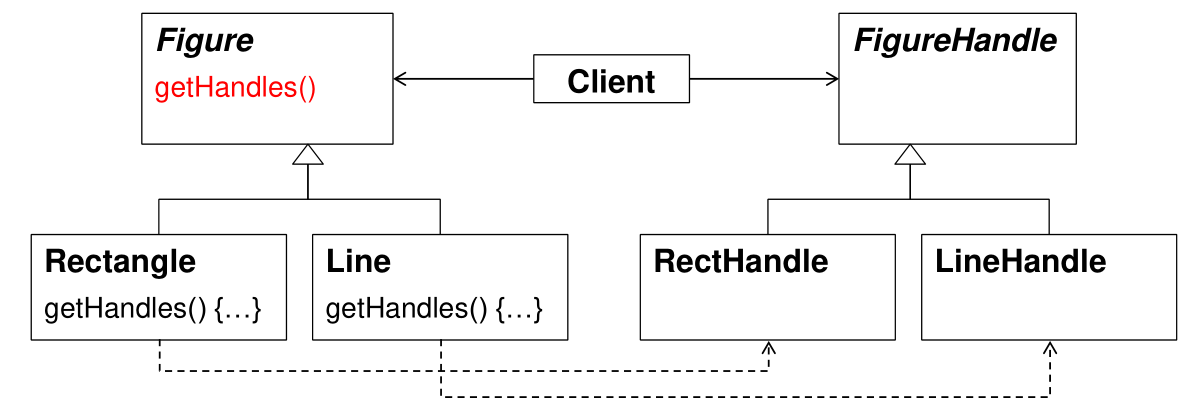
\includegraphics[width=1.0\columnwidth]{figures/factoryMethodHandles.png}
  \caption{}
  \label{fig:}
\end{figure}
\begin{defnbox}\nospacing
  \begin{defn}[GOF Definition]\label{defn:}
    Define an interface for creating an object, but let subclasses decide which class to instantiate. Factory Method lets a class defer instantiation to subclasses. 
  \end{defn}
\end{defnbox}
\begin{notebox}[Note]\nospacing
  People often use Factory Method as the standard way to create objects; but it isn't necessary if: the class that's instantiated never changes.
\end{notebox}
\begin{notebox}[Note]\nospacing
  The Factory Method pattern has commonly been misunderstood to mean any method whose sole purpose is to construct an object and return this created object. In most cases, this translates to a static method that abstracts the construction process of an object
\end{notebox}
\begin{partbox}[Participants]
  \begin{itemizenosep}
    \item \imp{Abstrac/Interface Product}: specifies type of product to be
  created e.g.\ HandleType
    \item \imp{Abstrac/Interface Creator}: Object that will instantiate the
  product may be
  \begin{itemize}
      \item an \javainline{interface} which includes one or more Factory
    Methods, as well as any number of other methods.
      \item an \javainline{abstract class}
    with defined methods or even a default implementation of the Factory Method that returns a default instance of Product. 
  \end{itemize}
    \item \imp{Concrete Creator}: creator class ($\neq$ factory)s that uses
    factory method \& returns different \javainline{ConcreteProduct} instances
    (that all implement the Product interface) depending on the the concrete
    creator. 
  \end{itemizenosep}
\end{partbox}
\begin{sectionbox}[Implementation]\nospacing
  \begin{itemizenosep}
      \item \imp{In a static method}: simplified version of factoryMethod
    (pattern):
    where the Creator hierarchy is reduced to a single class and the factory
    method is reduced to a single static method (rather than a method that is
    overridden for each of the possible products).\\
    The use of this \javainline{static method} allows for a single point of
    entry into a library. We use the class in order to obtain a conrete object.
    \begin{mintlinebox}{java}
      public class XmlHandlerFactory {
        public static XmlHandler createHandler() {
          return new XmlPrintHandler();
        }
      }
      |\optldots|
      XmlHandler handler = XmlHandlerFactory.createHandler();
    \end{mintlinebox}
      \item \imp{Sub classes}: as discussed above
      \item \imp{In an separate object} = \rdb{Abstract Factory pattern}
  \end{itemizenosep}
\end{sectionbox}
\begin{notebox}[Note: static approach]\nospacing
  assumes that the \javainline{XmlHandler} creator has enough knowledge to know
  which handler implementation is appropriate.
\end{notebox}
\begin{notebox}[Difference Abstrac Factroy]\nospacing
  Factory Method is similar to Abstract Factory but without the emphasis on families.
\end{notebox}
\begin{codeboxNl}[Product Interface]{java}
public interface EncryptionAlgorithm {
  public String encrypt(String plaintext);
}
\end{codeboxNl}
\begin{codeboxNl}[Concrete Product]{java}
public class Sha512EncryptionAlgorithm implements EncryptionAlgorithm {
  @Override
  public String encrypt(String plaintext) {
      return DigestUtils.sha512Hex(plaintext);
  }
}
\end{codeboxNl}
\begin{codeboxNl}[Abstract Creator]{java}
 public abstract class Encryptor {
  public void writeToDisk(String plaintext, String filename) {
      EncryptionAlgorithm encryptionAlgorithm = getEncryptionAlgorithm();
      String cyphertext = encryptionAlgorithm.encrypt(plaintext);
      |\optldots|
  }
  public abstract EncryptionAlgorithm getEncryptionAlgorithm();
} 
\end{codeboxNl}
\begin{codeboxNl}[ConcreteCreator]{java}
  public class Sha256Encryptor extends Encryptor {
    @Override
    public EncryptionAlgorithm getEncryptionAlgorithm() {
        return new Sha256CEncryptionAlgorithm();
    }
}
\end{codeboxNl}
\begin{sectionbox}[Implementation Issues]\nospacing
  \begin{itemizenosep}
      \item static factory implementations method cannot be overridden (as the
    method is static) $\Rightarrow$ can be compared to a \javainline{final factory method} \item Factory methods my be parameterized to describe the product it
    creates:
    \begin{mintlinebox}{java}
      Product createProduct(ProductID id)
    \end{mintlinebox}
    \item Factory Method in abstract base class may provide default return type.
  \end{itemizenosep}
\end{sectionbox}
%%% Local Variables:
%%% mode: latex
%%% TeX-master: "../formulary"
%%% End:

\subsection{Abstract Factory Pattern}
\label{subsubsec:Abstractfactory}
\begin{figure}[H]
  \centering
  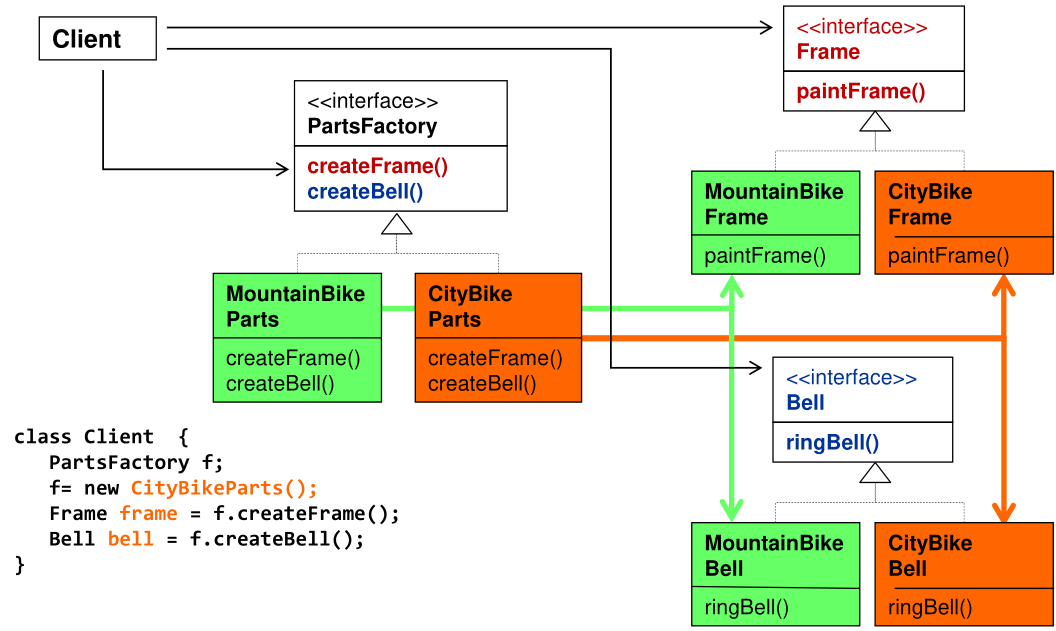
\includegraphics[width=1.0\columnwidth]{figures/abstractFactory.png}
\end{figure}
\begin{intentbox}[Intent]\\
Provide an interface for creating families of related or dependent objects without specifying their concrete classes.\\
  \rdb{Abstract Factory}=\rdb{Abstract Method}+\rdb{Strategy Pattern}\\
\end{intentbox}
\begin{partbox}\nospacing
  \begin{itemizenosep}
      \item \imp{Abstract/Interface Factory}: declares methods in order to
    create products of a certain family by:
    \begin{itemize}
        \item declaring an interface operations that create abstract products.
      \begin{mintlinebox}{java}
        interface Factory{
          intA createA();
          intB createB();
       }  
      \end{mintlinebox}
        \item declaring an abstract class that provides methods to produce
      abstract products
      \begin{mintlinebox}{java}
        abstract class Factory{
          public abstract intA createA();
          public abstract intB createB();
        }
      \end{mintlinebox}
    \end{itemize}
    $\Rightarrow$ methods to create product must share common interface:
    \begin{mintlinebox}{java}
      intA createProdA();
    \end{mintlinebox}
      \item \imp{Concrete Factories}: implements operations to create concrete
    products.
      \item \imp{Abstract/Interface Product}: declares an interface for a type
    of product. 
      \item \imp{Concrete Products}: products to be created by the corresponding
    ConcreteFactory;\\
    Need to implement the corresponding product interface in order to be
    consistent with the factories.
      \item \imp{Client}: Uses a factory in order to obtain products of a
    certain family.\\
    \imp{Note}: this may 
  \end{itemizenosep}
\end{partbox}
\subsubsection{Where is the concrete Factory}
\begin{sectionbox}\nospacing
 \begin{itemize}
     \item Directly used by client
     \item by another class that uses e.g.\ factory method and singleton 
 \end{itemize} 
\subsubsection{Who creates the concrete factory?}
\end{sectionbox}
\begin{itemizenosep}
    \item \imp{Externally}:
  \begin{mintlinebox}{java}
		CurrentFactory.setFactory(new Factory1());
  \end{mintlinebox}
    \item \imp{Internally}:
  \begin{mintlinebox}{java}
		CurrentFactory.setFactory(new Factory1());
  \end{mintlinebox}
    \item \imp{Automatically upon loading}:
  \begin{mintlinebox}{java}
		class Factory1 implements Factory {
      public A createA() { ... }
      public B createB() { ... }
      static {
        CurrentFactory.setFactory(new Factory1());
      }
      private Factory1() { };
    }
  \end{mintlinebox}
\end{itemizenosep}
\begin{defnbox}\nospacing
  \begin{defn}[Static Block]\label{defn:staticBlock}
    Will be called only once at initialization even-though if we call the
    constructor multiple times.
  \end{defn}
\end{defnbox}
\subsubsection{Difference factory Method and abstractFactory}
\begin{sectionbox}\nospacing
  The main difference between a "factory method" and an "abstract factory" is that the factory method is a single method, and an abstract factory is an object. I think a lot of people get these two terms confused, and start using them interchangeably. I remember that I had a hard time finding exactly what the difference was when I learnt them.
\end{sectionbox}
\begin{sectionbox}[Factory Method Paradigm]\nospacing
  \ldots the Factory Method pattern uses inheritance and relies on a subclass to
  handle the desired object instantiation.
\end{sectionbox}
\begin{sectionbox}[Abstract Factory Paradigm]\nospacing
  With the Abstract Factory pattern, a class delegates the responsibility of
  object instantiation to another object via composition.\\
  What they're saying is that there is an object A, who wants to make a Foo object. Instead of making the Foo object itself (e.g., with a factory method), it's going to get a different object (the abstract factory) to create the Foo object.
\end{sectionbox}
\begin{notebox}[Factory vs. DI]\nospacing
  When using a factory your code is still actually responsible for creating objects. By DI you outsource that responsibility to another class or a framework, which is separate from your code.
\end{notebox}
%%% Local Variables:
%%% mode: latex
%%% TeX-master: "../formulary"
%%% End:

\subsection{Singleton Pattern}
\label{subsubsec:singletonPattern}
\begin{intentbox}
  Insure that a class has only one instance at a time.
\end{intentbox}
\begin{sectionbox}[Idea: use only static variables methods]\nospacing
  \imp{Problems}:
  \begin{itemizenosep}
      \item Order in which static inializers are called is not determined
      \begin{mintlinebox}{java}
        class A {
          static { System.out.println("A()"); }
          static int x = B.x + 1;
        }
        class B {
          static { System.out.println("B()"); }
          static int x = A.x + 1;
        }

        public class Initialization {
          public static void main(String[] args) throws Exception {
            System.out.println("A.x = " + A.x);
            System.out.println("B.x = " + B.x);
          }
        }
      \end{mintlinebox}
      \item We may require run-time information
  \end{itemizenosep}
\end{sectionbox}
\begin{partbox}[Participants]
  Only final Singleton class that provides a private constructor.\\
  final such that the constructor cannot be overridden in a child class.
\end{partbox}
\subsubsection{Eager Initialization}
\begin{sectionbox}\nospacing
  \imp{Problem}: singleton is instantiated when the class is first accessed.\\
  If the class contains other \javainline{static} fields or methods we may
  create a costly object that we do not even need atm.
\begin{mintlinebox}{java}
  public final class Singleton {
  private Singleton() { }
    private static Singleton instance = new Singleton();
      public static Singleton getInstance() {
      return instance;
    }
  }
\end{mintlinebox}
\end{sectionbox}
\subsubsection{Lazy Initialization}
\begin{sectionbox}\nospacing
Only create new instance if it does not already exist:
\begin{mintlinebox}{java}
public final class Singleton {
  private Singleton() { }
  private static Singleton instance = null;

  public static |\colorbox{Red}{synchronized}| Singleton getInstance() {
    if(instance == null) instance = new Singleton();
    return instance;
}
\end{mintlinebox}
\end{sectionbox}
\begin{notebox}[Problem]\nospacing
  \javainline{synchronized}: is important for thread safety but really expensive
  and we need to synchronize on every \javainline{getInstance}
\end{notebox}
\begin{sectionbox}[Solution: singleton with double checking]\nospacing
  Tries to avoid costly synchronization by first checking synchronized.
  \begin{mintlinebox}{java}
		public class Singleton {
      private |\colorbox{Red}{volatile}| static Singleton instance;
      public static Singleton getInstance() {
        if(instance == null) {
          synchronized(Singleton.class) {
            if(instance == null) {
              instance = new Singleton();
            }
          }
        }
        return instance;
      }

      private Singleton() { /* initialization */ }
        // other methods
    }
  \end{mintlinebox}
\end{sectionbox}
\begin{notebox}[Note]\nospacing
  Need to volatile so that compiler does not optimize away our if.
\end{notebox}
\subsubsection{Holder Initialization}
\begin{sectionbox}\nospacing
  Instance is created upon first access of getInstance (lazy instantiation) and
  not on access of singleton static fields. 
\begin{mintlinebox}{java}
public final class Singleton {
  private static class Holder {
    private static final Singleton INSTANCE = new Singleton();
  }
  private Singleton() { }

  public static Singleton getInstance() {
    return Holder.INSTANCE;
  }
}
\end{mintlinebox}
\end{sectionbox}
%%% Local Variables:
%%% mode: latex
%%% TeX-master: "../formulary"
%%% End:

\subsection{Builder Pattern}
\label{subsubsec:builderPattern}
\begin{figure}[H]	
  \centering
    \resizebox{\linewidth}{!}{\tikzset{font=\Huge}\documentclass{standalone}
\usepackage{tikz}
\usepackage{aeguill}
\begin{document}
% generated by Plantuml 1.2018.12      
\definecolor{plantucolor0000}{RGB}{254,254,206}
\definecolor{plantucolor0001}{RGB}{168,0,54}
\definecolor{plantucolor0002}{RGB}{173,209,178}
\definecolor{plantucolor0003}{RGB}{0,0,0}
\definecolor{plantucolor0004}{RGB}{180,167,229}
\definecolor{plantucolor0005}{RGB}{255,255,255}
\begin{tikzpicture}[yscale=-1
,pstyle0/.style={color=plantucolor0001,fill=plantucolor0000,line width=1.5pt}
,pstyle1/.style={color=plantucolor0001,fill=plantucolor0002,line width=1.0pt}
,pstyle2/.style={color=plantucolor0001,line width=1.5pt}
,pstyle4/.style={color=plantucolor0001,line width=1.0pt}
,pstyle5/.style={color=plantucolor0001,fill=plantucolor0001,line width=1.0pt}
]
\draw[pstyle0] (6pt,14pt) rectangle (97.7882pt,87.6094pt);
\draw[pstyle1] (21pt,30pt) ellipse (11pt and 11pt);
\node at (21pt,30pt)[]{\textbf{\Large C}};
\node at (35pt,23.0156pt)[below right,color=black]{Director};
\draw[pstyle2] (7pt,46pt) -- (96.7882pt,46pt);
\node at (12pt,50pt)[below right,color=black]{builder};
\draw[pstyle2] (7pt,66.8047pt) -- (96.7882pt,66.8047pt);
\node at (12pt,70.8047pt)[below right,color=black]{construct()};
\draw[pstyle0] (133.5pt,14pt) rectangle (218.613pt,87.6094pt);
\draw[color=plantucolor0001,fill=plantucolor0004,line width=1.0pt] (148.5pt,30pt) ellipse (11pt and 11pt);
\node at (148.5pt,30pt)[]{\textbf{\Large I}};
\node at (162.5pt,23.0156pt)[below right,color=black]{\textit{Builder}};
\draw[pstyle2] (134.5pt,46pt) -- (217.613pt,46pt);
\draw[pstyle2] (134.5pt,54pt) -- (217.613pt,54pt);
\node at (139.5pt,58pt)[below right,color=black]{buildPartA()};
\node at (139.5pt,70.8047pt)[below right,color=black]{buildPartB()};
\draw[pstyle0] (254pt,8pt) rectangle (404.1647pt,94.4141pt);
\draw[pstyle1] (269pt,24pt) ellipse (11pt and 11pt);
\node at (269pt,24pt)[]{\textbf{\Large C}};
\node at (283pt,17.0156pt)[below right,color=black]{ConcreteBuilder};
\draw[pstyle2] (255pt,40pt) -- (403.1647pt,40pt);
\draw[pstyle2] (255pt,48pt) -- (403.1647pt,48pt);
\node at (260pt,52pt)[below right,color=black]{buildPartA()};
\node at (260pt,64.8047pt)[below right,color=black]{buildPartB()};
\node at (260pt,77.6094pt)[below right,color=black]{build() : Product};
\draw[pstyle0] (285pt,171pt) rectangle (372.9429pt,219pt);
\draw[pstyle1] (300pt,187pt) ellipse (11pt and 11pt);
\node at (300pt,187pt)[]{\textbf{\Large C}};
\node at (314pt,180.0156pt)[below right,color=black]{Product};
\draw[pstyle2] (286pt,203pt) -- (371.9429pt,203pt);
\draw[pstyle2] (286pt,211pt) -- (371.9429pt,211pt);
\draw[pstyle4] (111.2669pt,51pt) ..controls (114.2576pt,51pt) and (117.2483pt,51pt) .. (120.2391pt,51pt);
\draw[pstyle5] (133.3523pt,51pt) -- (124.3523pt,47pt) -- (128.3523pt,51pt) -- (124.3523pt,55pt) -- (133.3523pt,51pt) -- cycle;
\draw[pstyle4] (128.3523pt,51pt) -- (120.3523pt,50.9999pt);
\draw[color=plantucolor0001,fill=white,line width=1.0pt] (98.0156pt,51pt) -- (104.0156pt,55pt) -- (110.0156pt,51pt) -- (104.0156pt,47pt) -- (98.0156pt,51pt) -- cycle;
\draw[pstyle4] (238.9028pt,51pt) ..controls (243.8091pt,51pt) and (248.7155pt,51pt) .. (253.6218pt,51pt);
\draw[pstyle4] (238.7325pt,57.9999pt) -- (218.7324pt,51pt) -- (238.7324pt,43.9999pt) -- (238.7325pt,57.9999pt) -- cycle;
\draw[pstyle4] (329pt,94.2047pt) ..controls (329pt,117.269pt) and (329pt,145.0532pt) .. (329pt,165.6047pt);
\draw[pstyle5] (329pt,170.6665pt) -- (333pt,161.6665pt) -- (329pt,165.6665pt) -- (325pt,161.6665pt) -- (329pt,170.6665pt) -- cycle;
\node at (330pt,125pt)[below right,color=black]{Creates};
\draw[color=black,fill=black,line width=1.0pt] (354.2469pt,146.1328pt) -- (357.2469pt,152.1328pt) -- (360.2469pt,146.1328pt) -- (354.2469pt,146.1328pt) -- cycle;
\end{tikzpicture}
\end{document}
}
\end{figure}
\begin{intentbox}[Intent]
  Separate the construction of a complex object from its representation so
that the same construction process can create different representations.
\end{intentbox}
\begin{partbox}[Participants]
  \begin{itemizenosep}
      \item \imp{Builder}: Object which is used to build other objects.
  \end{itemizenosep}
\end{partbox}
\begin{codeboxNl}{java}
public class Pizza {
  private final int size;
  private final boolean cheese, pepperoni, bacon;

  public |\colorbox{Red}{static}| class Builder {
    private final int size;  // required 
    private boolean cheese = false;  // optional
    private boolean pepperoni = false;
    private boolean bacon = false;
    private boolean pinapple = false;

    Builder(int size) { this.size = size; }

    Builder cheese(boolean c) { cheese = c; return this; }
    Builder pepperoni(boolean p) { pepperoni=p; return this; }
    Builder bacon(boolean b) { bacon = b; return this; }
    // return finished build pizza (create method)
    Pizza build() { return new Pizza(this); }
  }  

  public |\colorbox{Red}{static}| class HawaiBuilder {
    private final int size;  // required 
    private boolean cheese = HawaiChees;  // optional
    private boolean pinapple = true;

    Builder(int size) { this.size = size; }
    Pizza build() { return new Pizza(this); }
  }  

  private genericPizza(Builder builder) {
      size = builder.size;
      cheese = builder.cheese;
      pepperoni = builder.pepperoni;
      bacon = builder.bacon;
  }
}
\end{codeboxNl}
\begin{codeboxNl}[Usage]{java}
  Pizza pizza = new Pizza.|\colorbox{Red}{Builder}|(12).
                                .cheese(true)
                                .pepperoni(true)
                                .bacon(true)
                                .build();
  Pizza pizza = new Pizza.|\colorbox{Red}{HawaiBuilder}|(12);
\end{codeboxNl}
\subsubsection{General Example}
\label{subsubsec:}
\begin{codeboxNl}[Product]{java}
class Pizza {
    private String dough = "";
    private String sauce = "";
    private String topping = "";

    public void setDough(String dough) {
        this.dough = dough;
    }

    public void setSauce(String sauce) {
        this.sauce = sauce;
    }

    public void setTopping(String topping) {
        this.topping = topping;
    }
}
\end{codeboxNl}
\begin{codeboxNl}[Abstract Builder]{java}
abstract class PizzaBuilder {
    protected Pizza pizza;

    public Pizza getPizza() {
        return pizza;
    }

    public void createNewPizzaProduct() {
        pizza = new Pizza();
    }

    public abstract void buildDough();
    public abstract void buildSauce();
    public abstract void buildTopping();
}
\end{codeboxNl}
\begin{codeboxNl}[Concrete Builder]{java}
class HawaiianPizzaBuilder extends PizzaBuilder {
    public void buildDough() {
        pizza.setDough("cross");
    }

    public void buildSauce() {
        pizza.setSauce("mild");
    }

    public void buildTopping() {
        pizza.setTopping("ham+pineapple");
    }
}

\end{codeboxNl}
\begin{codeboxNl}[Concrete Builder]{java}
class SpicyPizzaBuilder extends PizzaBuilder {
    public void buildDough() {
        pizza.setDough("pan baked");
    }

    public void buildSauce() {
        pizza.setSauce("hot");
    }

    public void buildTopping() {
        pizza.setTopping("pepperoni+salami");
    }
}
\end{codeboxNl}
\begin{codeboxNl}[Director]{java}
class Waiter {
    private PizzaBuilder pizzaBuilder;

    public void setPizzaBuilder(PizzaBuilder pb) {
        pizzaBuilder = pb;
    }

    public Pizza getPizza() {
        return pizzaBuilder.getPizza();
    }

    public void constructPizza() {
        pizzaBuilder.createNewPizzaProduct();
        pizzaBuilder.buildDough();
        pizzaBuilder.buildSauce();
        pizzaBuilder.buildTopping();
    }
}
\end{codeboxNl}
\begin{codeboxNl}[Customer]{java}
public class PizzaBuilderDemo {
    public static void main(String[] args) {
        Waiter waiter = new Waiter();
        PizzaBuilder hawaiianPizzabuilder = new HawaiianPizzaBuilder();
        PizzaBuilder spicyPizzaBuilder = new SpicyPizzaBuilder();

        waiter.setPizzaBuilder( hawaiianPizzabuilder );
        waiter.constructPizza();

        Pizza pizza = waiter.getPizza();
    }
}
\end{codeboxNl}
%%% Local Variables:
%%% mode: latex
%%% TeX-master: "../formulary"
%%% End:

\section{Structural Patters}
\label{subsubsec:Behavirol}
\section{Creational Patters}
\label{subsubsec:Behavirol}
% % ======================================================================
% % Todo
% % ======================================================================
% %%% Local Variables:
%%% mode: latex
%%% TeX-master: t
%%% End:

% \add{Method type bindining exercise 2/slides/more research}
\add{Nested Classes/Anonymous functions}
$https://www.tutorialspoint.com/java/java_innerclasses.htm$
\add{Java generics, generics with questionmark and extends.}
%%% Local Variables:
%%% mode: latex
%%% TeX-master: "../formulary"
%%% End:

% ==============================================================================
% Document end
% ==============================================================================
\end{document}




%%% Local Variables:
%%% mode: latex
%%% TeX-master: t
%%% TeX-command-extra-options: "-shell-escape"
%%% End:
